\documentclass[12pt]{article}
\usepackage{graphicx} % Required for inserting images
\usepackage[a4paper, inner= 1.5in, outer= 1in, top= 1in, bottom= 1in]{geometry}
\usepackage[onehalfspacing]{setspace} % to create a half spacing of 1.5 in
% \thispagestyle{}
\usepackage{ragged2e}
\usepackage{times}
\usepackage{fancyhdr}
\usepackage{url}

\fancyhf{}
\pagenumbering{arabic}



\newcommand{\theinstitute}{Institute of Engineering}
\newcommand{\thecampus}{Lalitpur Engineering College}
\newcommand{\thedepartment}{Department of Computer Engineering}
\newcommand{\thedepartmentAddress}{Kathmandu, Nepal}
\newcommand{\thedepartmentFullAddress}{Chakupat, Lalitpur, Nepal}
\newcommand{\theprogramcoordinator}{Er. Bisikha Subedi}
\newcommand{\theHOD}{Er. Praches Acharya}
\newcommand{\thesupervisor}{Er. Bishika Subedi}



\newcommand{\thetitle}{DefaceLab:  DeepFake Detection using Deep Learning}
\newcommand{\theauthor}{ABHISHEK NEUPANE [LEC076BCT002]
    \\RABINDRA ADHIKARI [LEC076BCT025]
    \\SANJISH MAHARJAN [LEC076BCT032]
    \\SUSHIL KAFLE [LEC076BCT045]}


\usepackage{amssymb}
\usepackage{graphicx}
\usepackage{amsmath}
\usepackage{algorithm}
\usepackage[noend]{algpseudocode}
\usepackage{datetime}
\usepackage{subcaption}
\usepackage{caption}
\captionsetup{font=it}
\usepackage{titlesec}
\usepackage{tocloft}
\usepackage{setspace}
\usepackage{titletoc}

% Set font size for titles in Table of Contents, List of Figures, and List of Tables
\renewcommand{\contentsname}{\normalfont\fontsize{14}{16}\bfseries Table of Contents}
\renewcommand{\listfigurename}{\normalfont\fontsize{14}{16}\bfseries List of Figures}
\renewcommand{\listtablename}{\normalfont\fontsize{14}{16}\bfseries List of Tables}


% Redefine sectioning commands to change font size
\titleformat{\section}{\normalfont\fontsize{14}{16}\bfseries}{\thesection}{1em}{}
\titleformat{\subsection}{\normalfont\fontsize{12}{16}\bfseries}{\thesubsection}{1em}{}
\titleformat{\subsubsection}{\normalfont\fontsize{12}{16}\bfseries}{\thesubsubsection}{1em}{}
\onehalfspacing
\setstretch{1.5}

\begin{document}
% \renewcommand{\cftfigpresnum}{\begin{lrbox}{\@tempboxa}}
%     \renewcommand{\cftfigaftersnum}{\end{lrbox}}
% \renewcommand{\numberline}[1]{}
\cftsetindents{figure}{0em}{3em}
\cftsetindents{table}{0em}{3em}
\begin{center}

    \thispagestyle{empty}
    {\fontsize{16 pt}{12} \selectfont\textbf{TRIBHUVAN UNIVERSITY} \\
        \textbf{INSTITUTE OF ENGINEERING}} \\
    \vspace{0.3 in}

    
\includegraphics[width= 3in ]{img/leclogo21.png} \\
    \vspace{0.05 in}
    LALITPUR ENGINEERING COLLEGE \\
    CHAKUPAT, LALITPUR \\

    \vspace{0.5 in}
    \textbf{ A PROPOSAL OF MAJOR PROJECT}\\
    {\fontsize{16 pt}{12} \selectfont \textbf{\thetitle}}\\
    \vspace{1.1 in}
    \textbf{ SUBMITTED BY}  \\
    {\theauthor} \\
    \vspace{1.1 in}
    \textbf{ SUBMITTED TO}  \\
    DEPARTMENT OF COMPUTER ENGINERING \\
    \vspace{1 in}
    \textbf{Bhadra 2080} \\
\end{center}
\begin{center}
    \linespread{1.6}
    \thispagestyle{empty}
    
\includegraphics[width= 3in ]{img/leclogo21.png} \\
    \vspace{0.05 in}
    {\fontsize{12 pt}{12} \selectfont\textbf{TRIBHUVAN UNIVERSITY} \\
        \textbf{INSTITUTE OF ENGINEERING} \\
        % \vspace{0.3 in}
        \textbf{LALITPUR ENGINEERING COLLEGE}} \\
    % CHAKUPAT, LALITPUR} \\

    \vspace{0.5 in}
    \textbf{A project Report}\\
    {\fontsize{12 pt}{12} \selectfont\textbf{On}\\}
    {\fontsize{12 pt}{12} \selectfont \textbf{\thetitle}}\\
    \vspace{0.4 in}
    \textbf{ Submitted By:}  \\
    {\theauthor} \\
    \vspace{0.3 in}
    \textbf{ Submitted To:}  \\
    Department of Computer Engineering \\
    Lalitpur Engineering College \\
    Chakupat, Lalitpur \\

    \vspace{0.2in}
    In partial fulfillment for the award of the
    Bachelor's Degree in Computer Engineering

    \vspace{0.2in}
    \textbf{Under the Supervision of} \\
    \thesupervisor\\
    \vspace{0.2in}
    \thedate

\end{center}

\newpage

\addcontentsline{toc}{section}{DECLARATION} % Add Acknowledgement to TOC
\pagenumbering{roman}
\section*{DECLARATION}
% \vspace{0.5cm}

We hereby declare that the report of the project entitled \textbf{"DefaceLab:  DeepFake Detection using Vision Transformer"} which is
being submitted to the \textbf{\thedepartment}, \textbf{\thecampus}, in the partial fulfillment of the requirements for the award
of the Degree of Bachelor in \textbf{Computer Engineering}, is a bonafide report of the work carried out by us. The materials
contained in this report have not been submitted to any University or Institution for
the award of any degree and we are the only author of this complete work and no
sources other than the listed here have been used in this work.

\vspace{2cm}
\noindent Abhishek Neupane [LEC076BCT002] \space{}\space{}\space{}\space{}\space{}\space{}  \line(1,0){150}\\
\vspace{0.1cm}

\noindent Rabindra Adhikari [LEC076BCT025] \space{}\space{}\space{}\space{}\space{}\space{}\space{} \line(1,0){150} \\
\vspace{0.1cm}

\noindent Sanjish Maharjan [LEC076BCT032]\space{}\space{}\space{}\space{}\space{}\space{}\space{}\space{}\space{} \line(1,0){150} \\
\vspace{0.1cm}

\noindent Sushil Kafle [LEC076BCT045]\space{}\space{}\space{}\space{}\space{}\space{}\space{}\space{} \space{}\space{}\space{}\space{}\space{}\space{}\space{}\space{}\space{}\line(1,0){150}\\


\vspace{0.7cm}
\noindent \textbf{Date: }\thedate \\

\newpage

\addcontentsline{toc}{section}{CERTIFICATE OF APPROVAL} % Add Acknowledgement to TOC
\section*{CERTIFICATE OF APPROVAL}
\begingroup
\setlength{\parskip}{0pt}
% \vspace{0.5cm}

The undersigned certify that they have read and recommended to the \textbf{\thedepartment,  \thecampus}, a major
project work entitled \textbf{“DefaceLab:  DeepFake Detection using Vision Transformer"} submitted by \textbf{Abhishek Neupane, Rabindra Adhikari, Sanjish Maharjan, Sushil Kafle} in partial fulfillment for the award of Bachelor’s
Degree in Computer Engineering. The Project was carried out
under special supervision and within the time frame prescribed by the syllabus.

\vspace{0.7cm}

\noindent We found the students to be hardworking, skilled and ready to undertake any related
work to their field of study and hence we recommend the award of partial fulfillment
of Bachelor’s degree of Computer Engineering.

\vspace{0.7cm}

\noindent \line(1,0){250}

\noindent Project Supervisor \\
\thesupervisor \\
\thedepartment, \thecampus

% \noindent \line(1,0){200}

\vspace{0.5cm}
\noindent \line(1,0){250}\\
\noindent External Examiner \\

\noindent \line(1,0){250}\\

\vspace{0.3cm}

\noindent \line(1,0){250}

\noindent Project Co-ordinator \\
\theprogramcoordinator \\
\thedepartment, \thecampus

\vspace{0.4cm}

\noindent \line(1,0){250}

\noindent \theHOD \\
Head of the Department, \\
\thedepartment, \thecampus

\vspace{0.3cm}

\noindent \thedate
\endgroup
\newpage
\addcontentsline{toc}{section}{COPYRIGHT} % Add Acknowledgement to TOC
\section*{COPYRIGHT}
\vspace{0.5cm}

The author has agreed that the library, \thedepartment, \thecampus, may make this project
work freely available for inspection. Moreover the author has agreed that the
permission for extensive copying of this project work for scholarly purpose may be
granted by the professor(s), who supervised the project work recorded herein or, in
their absence, by the Head of the Department, wherein this project work was done. It
is understood that the recognition will be given to the author of this project work and
to the \thedepartment, \thecampus \ in any use of the material of this project work. Copying of publication or other use of
this project work for financial gain without approval of the \thedepartment, \theinstitute, \thecampus \ and author’s
written permission is prohibited.\\
\\
Request for permission to copy or to make any use of the material in this thesis in
whole or part should be addressed to:\\
\\
\thedepartment\\
\thecampus\\
\thedepartmentFullAddress


\newpage


\addcontentsline{toc}{section}{ACKNOWLEDGEMENT} % Add Acknowledgement to TOC

% \pagenumbering{Roman}
\section*{ACKNOWLEDGEMENT}
\justify
We would like to acknowledge our indebtedness and render our warmest thanks to the project coordinator and our project supervisor {\thesupervisor}, who provided us with the helpful guidance in this project. Her immense knowledge, profound expertise, and friendly guidance have been invaluable throughout all stages of the work. We are grateful to the Department of  Computer Engineering, {\thecampus} for their help and suggestions in the selection and hopeful execution of this project. Finally, we would like to express our sincere appreciation to the department for helping us hone our skills through this project.\\

\vspace{0.6in}
\noindent {\theauthorsmall}



\newpage

\addcontentsline{toc}{section}{ABSTRACT} % Add Abstract to TOC
\begin{center}
    
    
    \pagenumbering{Roman}
    \section*{ABSTRACT}
    \justify
    Deepfakes are realistic-looking fake media generated by deep-learning algorithms that iterate through large datasets until
    they have learned how to solve the given problem (i.e., swap faces or objects in video and digital content). The massive generation
    of such content and modification technologies is rapidly affecting the quality of public discourse and the safeguarding of
    human rights. Deepfakes are being widely used as a malicious source of misinformation in court that seek to sway a court’s decision.
    Because digital evidence is critical to the outcome of many legal cases, detecting deepfake media is extremely important and in high demand in digital forensics.
    As such, it is important to identify and build a classifier that can accurately distinguish between authentic and disguised media, especially in facial-recognition systems
    as it can be used in identity protection too. In this work, we compare the most common, state-of-the-art face-detection classifiers such as Custom CNN, VGG19, and DenseNet-121
    using an augmented real and fake face-detection dataset. Data augmentation is used to boost performance and reduce computational resources. Our preliminary results indicate that VGG19 has the best performance
    and highest accuracy of 95\% when compared with other analyzed models.\\
    \vspace{3 in}
    \\ \textit{Keywords: deepfake detection; digital forensics; media forensics; deep learning; VGG19; face-image manipulation}
    
    
\end{center}
\newpage

\tableofcontents
\newpage


\listoffigures
\newpage
\listoftables
\newpage

\section*{List of Abbreviations}
\begin{table}[h]

    \renewcommand{\arraystretch}{1.5}
    \begin{tabular}{@{}p{0.3\linewidth}p{0.6\linewidth}@{}}
        AUC     & Area Under the Curve              \\
        CNN     & Convolutional Neural Network      \\
        DFD     & Data Flow Diagram                 \\
        ELU     & Exponential Linear Unit           \\
        FN      & False Negative                    \\
        FP      & False Positive                    \\
        FPR     & False Positive Rate               \\
        FPS     & Frames Per Second                 \\
        GANs    & Generative Adversarial Networks   \\
        GELU    & Gaussian Error Linear Unit        \\
        JWT     & JSON Web Token                    \\
        KDE     & Kernel Density Estimation         \\
        MHA     & Multi-Head Attention              \\
        MLP     & Multi-Layer Perceptron            \\
        MSA     & Multihead Self-Attention          \\
        RELU    & Rectified Linear Unit             \\
        RMSprop & Root Mean Square Propagation      \\
        RNN     & Recurrent Neural Network          \\
        ROC     & Receiver Operating Characteristic \\
        SA      & Self-Attention                    \\
        SVM     & Support Vector Machine            \\
        TN      & True Negative                     \\
        TP      & True Positive                     \\
        TPR     & True Positive Rate                \\
        ViT     & Vision Transformer                \\
    \end{tabular}
\end{table}
% \thispagestyle{empty}



\pagenumbering{arabic}
\section{INTRODUCTION}
In the last few years, cybercrime, which accounts for a 67\% increase in the incidents of security breaches, has been one of the most challenging problems that national security systems have had to deal with worldwide [1].
Deepfakes (i.e., realistic-looking fake media that has been generated by deep-learning algorithms) are being widely used to swap faces or objects in video and digital content. This artificial intelligence-synthesized
content can have a significant impact on the determination of legitimacy due to its wide variety of applications and formats that deepfakes present online (i.e., audio, image and video).
Considering the quickness, ease of use, and impacts of social media, persuasive deepfakes can rapidly influence millions of people, destroy the lives of its victims and have a negative impact on society in general [1].
\\ The generation of deepfake media can have a wide range of intentions and motivations, from revenge porn to political fake news..
Deepfakes have also been published to falsify satellite images with non-existent landscape features for malicious purposes [3].
There are numerous captivating applications of deepfakery in video compositing and transfiguration in portraits, especially in identity protection as it can replace faces in photographs with ones from a collection of stock images.
Cyber-attackers, using various strategies other than deepfakery, are always aiming to penetrate identification or authentication systems to gain illegitimate access. Therefore, identifying deepfake media using forensic methods remains
an immense challenge since cyber-attackers always leverage newly published detection methods to immediately incorporate them in the next generation of deepfake generation methods. With the massive usage of the Internet and social media,
and billions of images available on the Internet, there has been an immense loss of trust from social media users. Deepfakes are a significant threat to our society and to digital evidence in courts. Therefore, it is highly important to
obtain state-of-the-art techniques to identify deepfake media under criminal investigation.
As demonstrated in Table 1 (inspired by the figure presented in [1]), tampering of evidence, scams and frauds (i.e., fake news), digital kidnapping associated with ransomware blackmailing, revenge porn and political sabotage are among the
vast majority of types of deepfake activities with the highest level of intention to mislead [1].



\subsection{Background}
At present context of time, the rapid advancements in mobile camera technology and the widespread use of social media platforms have made it easier than ever to create and share digital pictures. Deep learning has played a crucial role in developing technologies that were previously unimaginable. One notable example is modern generative models, which can produce highly realistic images, speech, music, and video. These models have been applied in various fields, such as enhancing accessibility through text-to-speech technology and generating training data for medical imaging.
\\
\\
There will always be drawbacks to any technological breakthrough. Since deepfakes are still relatively new and expanding quickly, their excessive use as a result of rising human interest has resulted in misuse of this technology. It is simple for widespread false information to proliferate among the populace when there is no controlling element and a weak mechanism in place to identify deep fakes.Since their initial emergence in late 2017, a variety of open-source deep fake generation techniques and tools have appeared, resulting in an increase in the amount of synthetic media clips. Others may be destructive to people and society, even though many are probably intended to be amusing. Due to the accessibility of editing tools and the strong demand for topic expertise, false digital contents have been growing in number and in realism up until recently.
\\
\\
Deep fakes are now widely disseminated on social media platforms, which encourages spamming and the spread of false information. Just picture a deep fake image of Donald Trump getting arrested which was trending on twitter or a deep fake of a well-known celebrity assaulting their supporters.
These types of misinformation can brainwash the audience and are awful and endanger and mislead the general public.
\\
\\
Deep fake detection plays a crucial part in overcoming such a circumstance. Therefore, we provide a novel deep learning-based method that can successfully separate artificial intelligence-generated fake contents from authentic digital materials. In order to identify deep fakes and stop them from spreading across the internet, it is crucial to develop technology that can detect deepfakes.

\subsection{Motivation}
According to the latest report from Home Security Heroes, the number of deepfake contents in the year 2023 has risen to 96,000, representing a growth of approximately 550\% compared to 2019. Even in technologically advanced regions such as the United Kingdom, only 32.9\% of the population expresses confidence in their ability to discern deepfake content. Notably, the corresponding figure for Nepal is considerably lower. Given this circumstance, the necessity to deploy an deepfake detection tool becomes apparent, functioning as a pivotal tool to address crimes and theft associated with deepfakes and  restrict the propagation of misinformation.\\
\begin{figure}[h]
    \centering
    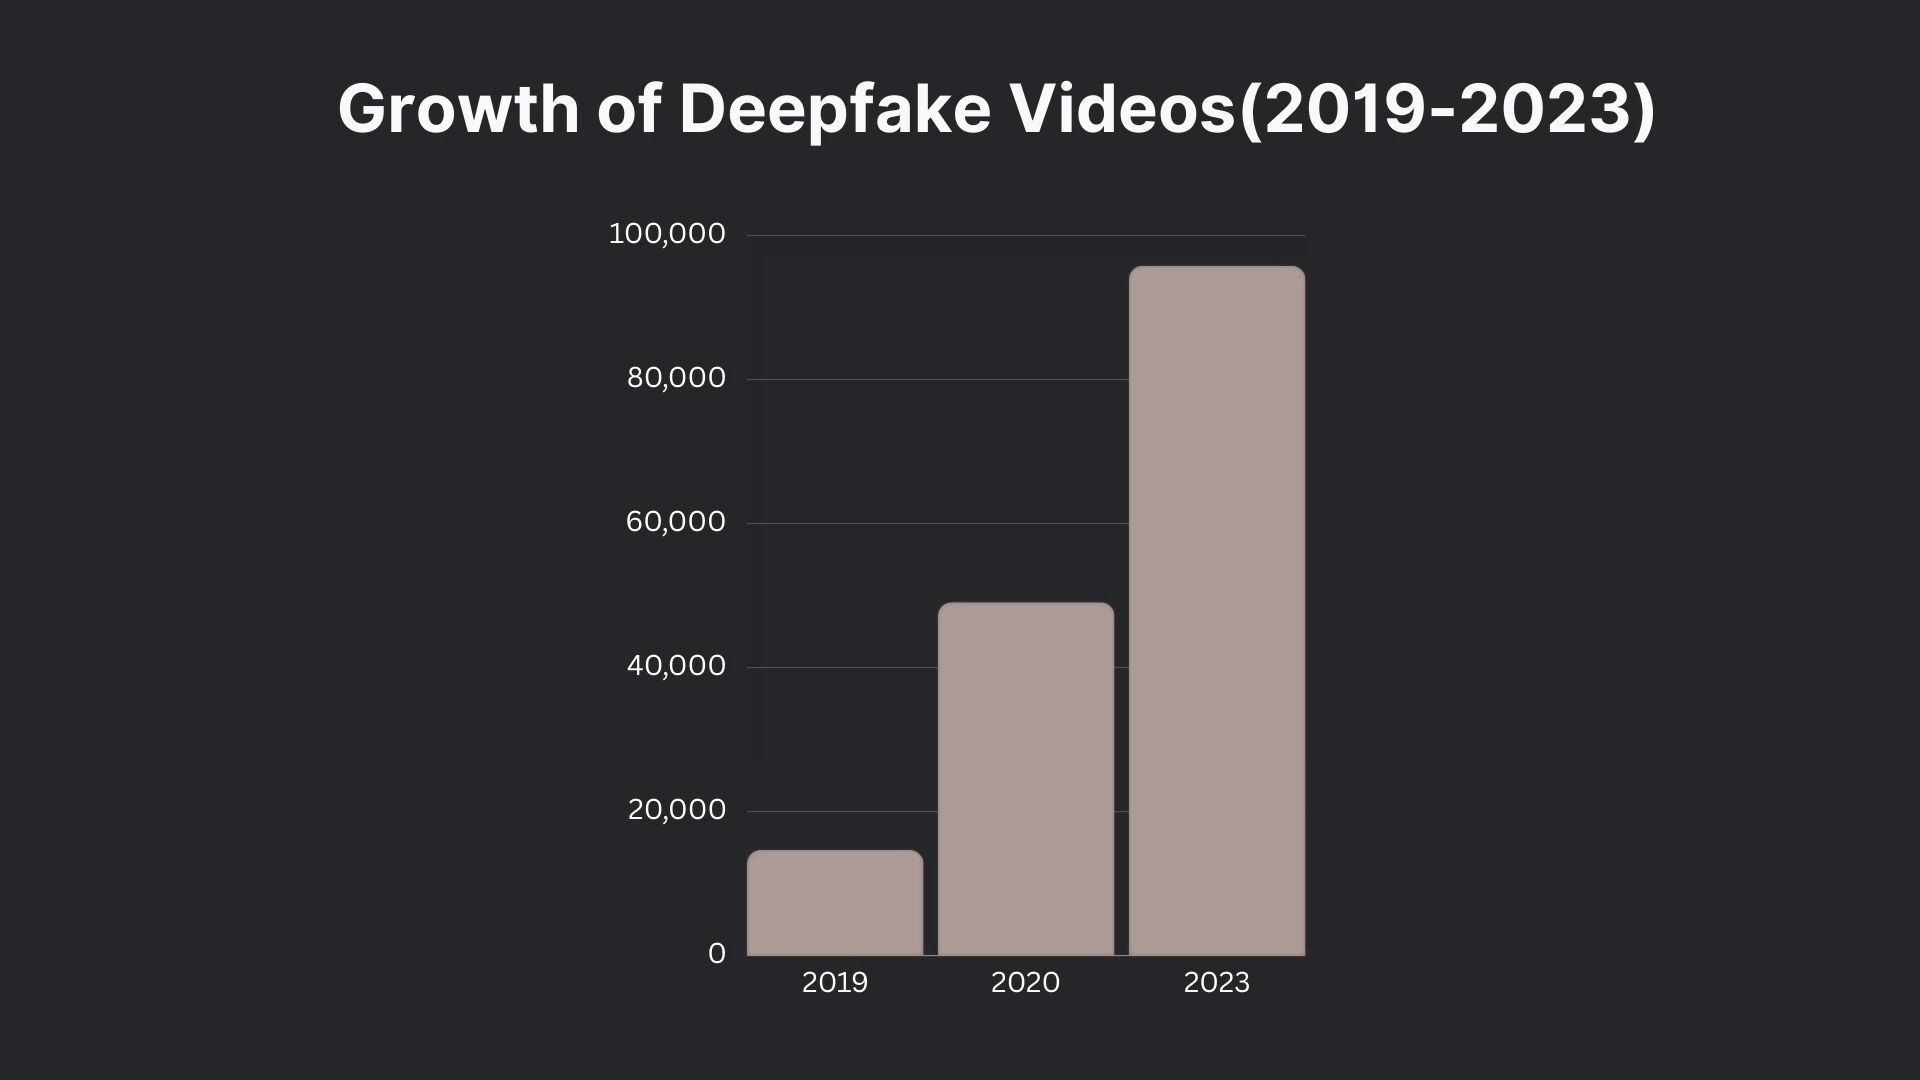
\includegraphics[width= 5.5in ]{img/deepfake-videos-growth.jpg}
    \caption{\textit{Deepfake videos growth over time}}
\end{figure}
\newpage



\subsection{Problem Statement}
With the help of visual effects, convincing modifications of digital photographs and videos have been proven for many years. However, new developments in deep learning have dramatically increased the realism of fake content and made it more widely available. These purportedly artificial intelligence-generated works of media are also known as "deepfakes". It is easy to create deep fakes utilizing artificial intelligence techniques. However, it is extremely difficult to identify these Deep Fakes.
Globally, it is found out that about 71\% of total population using internet do not know what a deepfake is. Just under a third of global consumers of internet say they are aware of deepfakes. In the past, there have been numerous instances of deep fakes being used to effectively incite political unrest, stage terrorist attacks, blackmail individuals, etc.
In North America alone, the proportion of deepfakes more than doubled from 2022 to 2023. This proportion jumped from 0.2\% to 2.6\% in the US and it is up from 0.1\% to 4.6\% in Canada and is rapidly growing\hyperref[ref5]{[5]}. Therefore, it becomes crucial to identify these deep fakes and monitor their spread through social media. Hence, with the growing curiosity we have taken a step forward in detecting the deep fakes using different transformer based models.

\subsection{Objectives}
\justify
\begin{itemize}
    \item Our project aims at discovering the distorted truth of the deep fakes.
    \item Our project will reduce the Abuses’ and misleading of the common people on
          the world wide web.
    \item Our project will distinguish and classify the video as deepfake or pristine.
    \item Provide a easy to use system for used to upload the video and distinguish
          whether the video is real or fake
\end{itemize}


\subsection{Project Scope and Applications}

Our project aims to address the prevalent issue of false videos in the realm of deepfake technology. Due to the limited availability of reliable detection tools, our main focus is on creating an accessible and user-friendly deepfake detection software. The primary objective is to curb the widespread dissemination of deepfakes by offering users a platform where they can easily upload digital content and distinguish between authentic and manipulated materials. Our goal is to contribute to a vigilant digital environment, promoting trust and authenticity in the face of evolving challenges posed by deceptive media content.

\noindent Our project helps in detecting and addressing deepfake content. However, it's crucial to recognize certain limitations. The effectiveness of our system  can be influenced by multiple factors like the characteristics of the input data. The detection of sequence of frames in videos cannot be tracked. Also, the inputs with tikas and face-masks are difficult to classify.

\noindent \textbf{Potential Application}

\begin{itemize}
    \item \textbf{Cybersecurity:} It can be integrated into cybersecurity systems to identify and prevent the spread of manipulated media that may pose security threats or deceive users.

    \item \textbf{Governmental Organizations:} Adoption within governmental organizations to safeguard against deepfake threats, especially in areas concerning national security, public figures, and official communications.

    \item \textbf{News and Journalism:} Integration into newsrooms and journalistic processes to verify media content, ensuring the dissemination of accurate information and maintaining the integrity of news reporting.

    \item \textbf{Education and Research:} Utilization in educational institutions for media literacy programs and research purposes, empowering students and researchers to critically assess the authenticity of visual content.
\end{itemize}



% \subsection{Originality of Project}
Our project has been integrated by combining our proprietary datasets with external ones, creating a local environment efficient foundation. We integrate a Vision Transformer (ViT) model, for the detection and recognition as we have fine-tuned with carefully selected and required parameters, enhancing our system's accuracy. This unique blend of datasets and ViT integration positions our project ensures efficiency and originality.

\subsection{Potential Application}


\subsection{Organization of Project Report}
\begin{itemize}
    \item Copyright: Acknowledgement of copyright information.
    \item Declaration: Formal declaration of originality of our project.
    \item Acknowledgement: Expression of gratitude for the support and assistance received during our project.
    \item Abstract: Includes the concise summary of our report.
    \item Introduction:
      \begin{itemize}
        \item Background: Presentation of the background information related to deepfake generation and detection.
        \item Motivation: Mention of our motivation behind choosing deepfake detection as our project.
        \item Problem Statement: Clear definition of the problem of deepfake content and the need for reliable detection.
        \item Objectives: Outline of the specific goals and objectives of our project.
        \item Scope: Definition of the boundaries of the project based on advantages and limitations.
        \item Potential Application: Exploration of potential real-world applications our system.
        \item Originality of Project: Highlighting of the unique aspects our project.
        \item Organization of Project Report: Overview of how the report is structured.
      \end{itemize}
    \item Literature Review:
      \begin{itemize}
        \item Existing Systems: Discussion of relevant existing systems for deepfake detection, including Deepware and DuckDuckGoose.
        \item Developed System: Description of the key features and components of our  developed system.
      \end{itemize}
    \item Feasibility Study:
      \begin{itemize}
        \item Economic Feasibility: Assessment of the economic viability of implementing the deepfake detection system.
        \item Operational Feasibility: Examination of the practicality and operational aspects of deploying the system.
        \item Technical Feasibility: Evaluation of the technical feasibility, considering the required technologies and resources.
      \end{itemize}
    \item Methodology:
      \begin{itemize}
        \item Software Development Life Cycle: Explanation of the chosen software development life cycle for the project.
        \item Deepfake: Definition of what deepfake is and its relevance to our project.
        \item Key Features Extraction: Explanation of the process of extracting key features, including abnormal patterns.
        \item Vision Transformer Architecture: Explanation the architecture.
        \item Benefits of Vision Transformer: Advantages of using Vision Transformer.
        \item Mathematical Modeling: Explanation of mathematical components such as activation function, loss function, and others involved.
        \item Dataset Collection: Collecting and preparing datasets for training and testing.
        \item Preprocessing: Outline of the preprocessing steps, including resize, augmentation, and normalization.
        \item Face Alignment Integration: Description of the integration of face alignment into the system.
        \item Algorithm: Presentation of our algorithm.
        \item Working Description: Elaborated explanation on our model.
        \item Model Training and Testing: Details of the process of training and testing of our model.
        \item Application Development: Description of the development of the mobile app, including frontend and backend components.
      \end{itemize}
      \item Block Diagrams:
      \begin{itemize}
        \item Use Case Diagram: Visual representation of the use cases.
        \item Sequence Diagram: Illustration of the sequence of interactions within the system.
        \item Dataflow Diagram: Presentation of the flow of data within the system.
        \item Class Diagram: Display of the class structure and relationships.
        \item Activity Diagram: Illustration of the workflow and activities within the system.
      \end{itemize}
  
    \item Result and Analysis:
      \begin{itemize}
        \item Parameters: Specification of the parameters used for the deepfake detection system.
        \item Evaluation: Presentation of the evaluation metrics and results.
        \item UI of Project: Showcase of the user interface of the developed mobile app.
      \end{itemize}
  
    \item Expected Outcomes:
      \begin{itemize}
        \item Discussion of the anticipated outcomes and impacts of our system.
      \end{itemize}
  
    \item Appendices:
      \begin{itemize}
        \item Inclusion of any additional information and supplementary materials.
      \end{itemize}
  \end{itemize}


\newpage

\section{LITERATURE REVIEW}

The facial manipulation is a techniques of altering someone's face in images or videos, often done using computer software. There are different types of facial manipulation techniques, each serving different purposes such as Face Morphing where two or more faces are blended together and create a seamless transition between them, Face Swapping, which involves replacing one person's face with another's while keeping the rest of the image intact, Attribute manipulation, where different attributes of face like nose, eyes, etc. are manipulated and Deepfakes, which uses advanced artificial intelligence and machine learning to create highly realistic digital contents by superimposing one person's face onto another person's body. These videos can convincingly mimic speech, expressions, and gestures, making them a source of concern for potential misinformation and privacy issues.
\\\\
The generation of deepfakes has had a rapid growth. Generating deepfakes involves using advanced technology to create fake videos or images that look very realistic. The deepfakes are created using deep learning techniques like Generative Adversarial Networks (GANs). The GAN technique involve two main components: a generator and a discriminator. The generator takes random noise as input and produces data, like images. The discriminator evaluates this generated data alongside real data and tries to tell them apart. As training progresses, the generator refines its output to become more convincing, while the discriminator becomes better at distinguishing real from fake. This competitive process pushes the generator to create increasingly realistic data that can be mistaken for real. As training progresses, the generator refines its output to become more convincing, while the discriminator becomes better at distinguishing real from fake. This competitive process pushes the generator to create increasingly realistic data that can be mistaken for real. 
\\\\
This remarkable advancement in deepfake technology underlines the desperate need for effective deepfake detection mechanisms. As these deceptively authentic videos, images, and audio recordings becomes more widespread, the risk of misinformation, deception, and breaches of privacy escalates hugely. Detecting deepfakes is a difficult challenge. However, researchers and experts are actively exploring diverse strategies to differentiate between these genuine and manipulated content. These strategies often involve detecting facial features for anomalies, identifying patterns and residuals in lighting and shadows, and uncovering distortions introduced during the manipulation process such as iris and pupil deformation.
\\\\
Since 2017, the Transformer has been very renowned as a new type of neural architecture for natural Language Processing which encodes the given input data into a powerful feature, with the help of attention mechanism.  With the research article published in 2017, named "Attention Is All You Need" [6], by taking it as a framework, numerous researches has been done recently upon the visions task as well [3]. This is where the Visual Transformer comes in. 
\\\\
While the Transformer Architecture has been a new standard for Natural Language Processing tasks, its application to computer vision remains limited. From many recent studies and researches done, the common points mentioned was that in vision, either the attention is applied in conjunction with convolution's networks, or used to replace certain components of convolutional network while keeping their overall structure in place [4].
The Transformer-liked architecture has been employed in the computer vision field in present context in three fundamental computer vision tasks, namely classification, detection and segmentation [2]. Our work lies within one of these fundamental tasks i.e the detection of artificially generated images of a human face.
\\\\
 The Visual Transformer has been gaining many contributions in recent years such that its capabilities has increased beyond the old traditional models. As a matter of fact, the Visual Transformer model has clear advantages over traditional models such as CNNs and RNNs in specific situations. It can process whole images in sections, which helps it understand the bigger picture. Also, it is good with working on different image sizes and tasks. 
 Training these models on big datasets first and then adjusting it for specific tasks makes it really flexible compared to the traditional model [5]. One of its key characteristics, self-attention, not only helps us understand how the model works but also reminds us to pick the right model based on the job, data, and what we have.
\\\\
In the Vision Transformer, the use of multi-headed self attention is used which allows the model to associate each individual testing attributes of input to run parallelly. The query, key and values vectors are used as the calculation attributes to calculate scores, ultimately gaining the softmax score for obtaining probability values and scaled scores for attention weights. These multi-headed attention are the concatenated for further processes. Before feeding the inputs in the ViT model, the input datas are to be preprocessed first. Initially, the frame extraction process is done, followed by the features abstraction. The features such as facial structure can be extracted with the help of Face Alignment Library. Then the input is normalized followed by resizing and patching, which provides a representation of NLP for the input to Vision Transformer [4].
\\\\
From recent researches done Vision Transformer (ViT) is deemed more suitable than Generative Adversarial Networks (GANs) for deepfake detection because Vision Transformer is specifically designed for image analysis tasks like classification. GANs are like artists that make fake pictures, but they're not as good at spotting fakes. Also, the tricks that make GANs create fakes can also fool themselves when looking for fakes. Vision transformer way of looking at pictures makes it a good choice for catching fake ones, because it's good at seeing small things that don't match up. Also, Vision Transformers (ViTs) have advantages over Recurrent Neural Networks (RNNs) in computer vision due to their parallel processing, better handling of long-range dependencies, efficient attention mechanisms, fewer assumptions about sequence structure, transfer learning capabilities, reduced overfitting, and interpretable representations. However, RNNs remain strong for sequential data tasks and short-term dependencies. Whereas against Convolutional Neural Networks (CNNs), ViT has advantages of efficient parallel processing, reduced invariance assumption, scalability, interpretable representations, fewer specialized architectures, and transfer learning. But CNNs is better for tasks requiring local features and spatial hierarchies.
\\\\
In summary, with all these distinct attributes and merits the Vision Transformer imposes itself significantly compared to others at present time and with understanding of the factors more compatible for our project, we have selected the Vision Transformer as the major model for our project development.


\newpage

\subsection{Existing Systems}
\subsubsection{Deepware}
Deepware.ai is an innovative company at the forefront of deepfake detection technology. They specialize in developing advanced AI-driven solutions to combat the spread of manipulated media content. With a team of expert researchers and engineers, Deepware.ai leverages state-of-the-art machine learning algorithms and deep neural networks to accurately identify deepfakes. Their cutting-edge technology, combined with a user-friendly approach, empowers individuals and organizations to protect themselves from the potentially harmful consequences of deepfakes. Deepware.ai's commitment to continuous improvement and staying ahead of evolving deepfake techniques positions them as a trusted leader in the field, offering reliable and scalable solutions that contribute to a safer digital landscape.
\begin{figure}[h]
    \centering
    
\includegraphics[width= 3in ]{img/deepware.png}
    \caption{\textit{Deepware}}
\end{figure}
\subsubsection{DuckDuckGoose}
\justify
DuckDuckGoose offers an open-source browser extension that keeps tabs on all websites you visit and alert you once manipulated media is detected.
Users should also appreciate the transparency of the DeepFake detector, as DuckDuckGoose provides detailed explanations for why a video was flagged to give you some insight on what to look for in a DeepFake.
The team behind the tool has been dedicated to sharing their research findings and encouraging participants from the community to contribute to building a more reliable model with higher accuracy.
\begin{figure}[h]
    \centering
    
\includegraphics[width= 3in ]{img/duckduckgoose.png}
    \caption{\textit{DuckDuckGoose}}
\end{figure}
\newpage
\newpage

\subsection{Proposed Systems}
Our Deepfake Detection System is an online tool designed to help people identify and deal with deepfake content. It focuses on providing strong detection capabilities for deepfakes. Users can use the system to analyze and detect potential deepfakes by submitting images. The system uses advanced algorithms and machine learning techniques to accurately identify manipulated or fake media. This helps users recognize and address the risks that come with deepfakes, such as spreading false information, committing fraud, or violating privacy. The deepfake detection system aims to empower users by giving them the tools they need to protect themselves and others from the harmful effects of encountering deepfakes. With the help of cutting-edge algorithms, the system assists users in detecting and raising awareness about deepfakes, making the digital world a safer and more informed place.
\newpage


\section{REQUIREMENT ANALYSIS}

\subsection{Functional Requirement}
The functional requirements of the system are:
\begin{enumerate}
    \item Authentication of users.
    \item User-friendly interface for uploading and detection.
    \item Image preprocessing.
    \item Mathematical Modeling and Implication.
    \item Model Development and training.
    \item Testing and Validation.

\end{enumerate}

\subsection{Non Functional Requirement}
\justify
These requirements are not needed by the system but are essential for the better
performance of software. The points below focus on the non-functional requirement of
the system.
\begin{enumerate}
    \item Reliability
    \item   Usability
    \item   Security
    \item   Portability
    \item   Speed and responsiveness
    \item   Performance
\end{enumerate}

\subsection{Feasibility Study}

\subsubsection{Economic feasibility}
This is a low-budget project with no development costs. The total expenditure of the
project is just computational power. The dataset and computational power required for
the project ware readily available. The computational power was provided by google
collab. So, the project was economically feasible. The system will be simple to
comprehend and use.

\subsubsection{Operational feasibility}
The project has been operationally feasible, as after the completion of our project, the operation through the developed can be carried out for the detection of deepfakes.

\subsubsection{Technical feasibility}
Our project's technical feasibility is assured by user-friendly tools like React Native, Keras and Google Colab. Keras simplified the implementation of our model, while Google Colab provides a collaborative and accessible environment for efficient development and training.

\subsection{System Development Tools}
Our Deepfake detection System requires and incorporates the tools which are listed below:
\begin{enumerate}
    \item Python Modules:
          \begin{itemize}
              \item NumPy:
                    Used for numerical operations and handling multi-dimensional arrays efficiently.
                    Employed in the data preprocessing phase for manipulation and transformation of image data.

              \item Keras:
                    A high-level deep learning API that simplifies the process of building and training neural networks.
                    Applied for building and training the deep fake detection model.

              \item Matplotlib:
                    Used for data visualization, helpful for understanding model performance and debugging.
                    Applied for plotting graphs and visualizing images during the analysis phase.
          \end{itemize}

    \item Google Colab:
          Provides a free cloud-based Jupyter notebook environment with GPU support, suitable for training deep learning models.
          Used for developing, training, and experimenting with the deep fake detection model.

    \item OpenCV:
          An open-source computer vision library that aids in image and video processing.
          Utilized for tasks like image loading, preprocessing, and post-processing during both training and inference phases.

    \item React Native:
          A framework for building mobile applications using JavaScript and React.
          Used for developing the mobile application interface for users to interact with the deep fake detection system.

    \item Expo Library:
          A set of tools and services for building React Native applications more efficiently.
          Enhances the development process and simplifies the deployment of the React Native application.

    \item Git/GitHub:
          Version control system for tracking changes in the codebase, collaborating with team members, and managing project versions.
          Used throughout the project for maintaining code integrity and facilitating collaboration.

    \item FastAPI:
          A modern, fast web framework for building APIs with Python 3.7+ based on standard Python type hints.
          Used for developing the backend API that connects the React Native application with the deep fake detection model.
\end{enumerate}

\newpage
\newpage


\section{SYSTEM ARCHITECTURE AND METHODOLOGY }
\subsection{Block Diagram}
\begin{figure}[h]
    \centering
    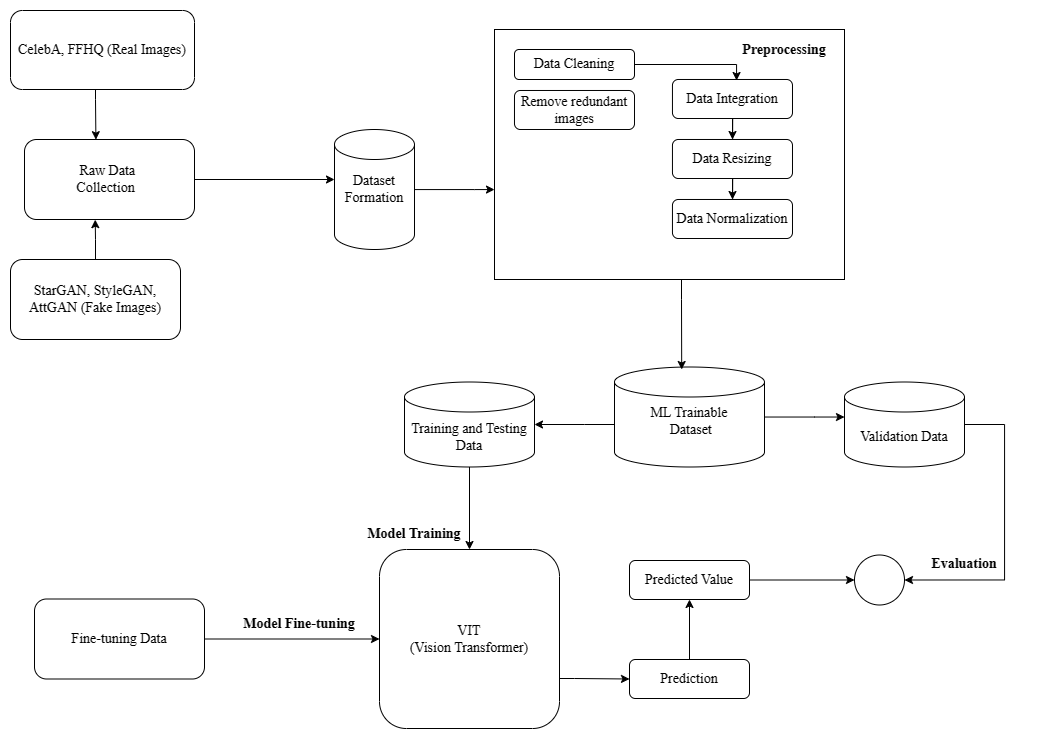
\includegraphics[width= 6.5in ]{img/Model_Architecture.drawio (4).png}
    \caption{{System Architecture}}

\end{figure}
\justify
The system architecture of our project involves multiple steps. Initially, the formation of datasets takes place as raw data are collected to training, testing and validation  The frames are extracted from the input video or obtained directly from an image. These frames then undergo face extraction, where faces are identified and cropped using face detection algorithms. The extracted faces are resized to a standardized size and undergo normalization to ensure consistent pixel values. The preprocessed face images are then fed into a deep learning model for classification. The model analyzes the features and patterns in the images to determine whether they are real or fake. Finally, the system produces the output, indicating the authenticity of the input video or image as either real or fake.

\newpage

\subsection{Use Case Diagram}
\begin{figure}[h]
    \centering
    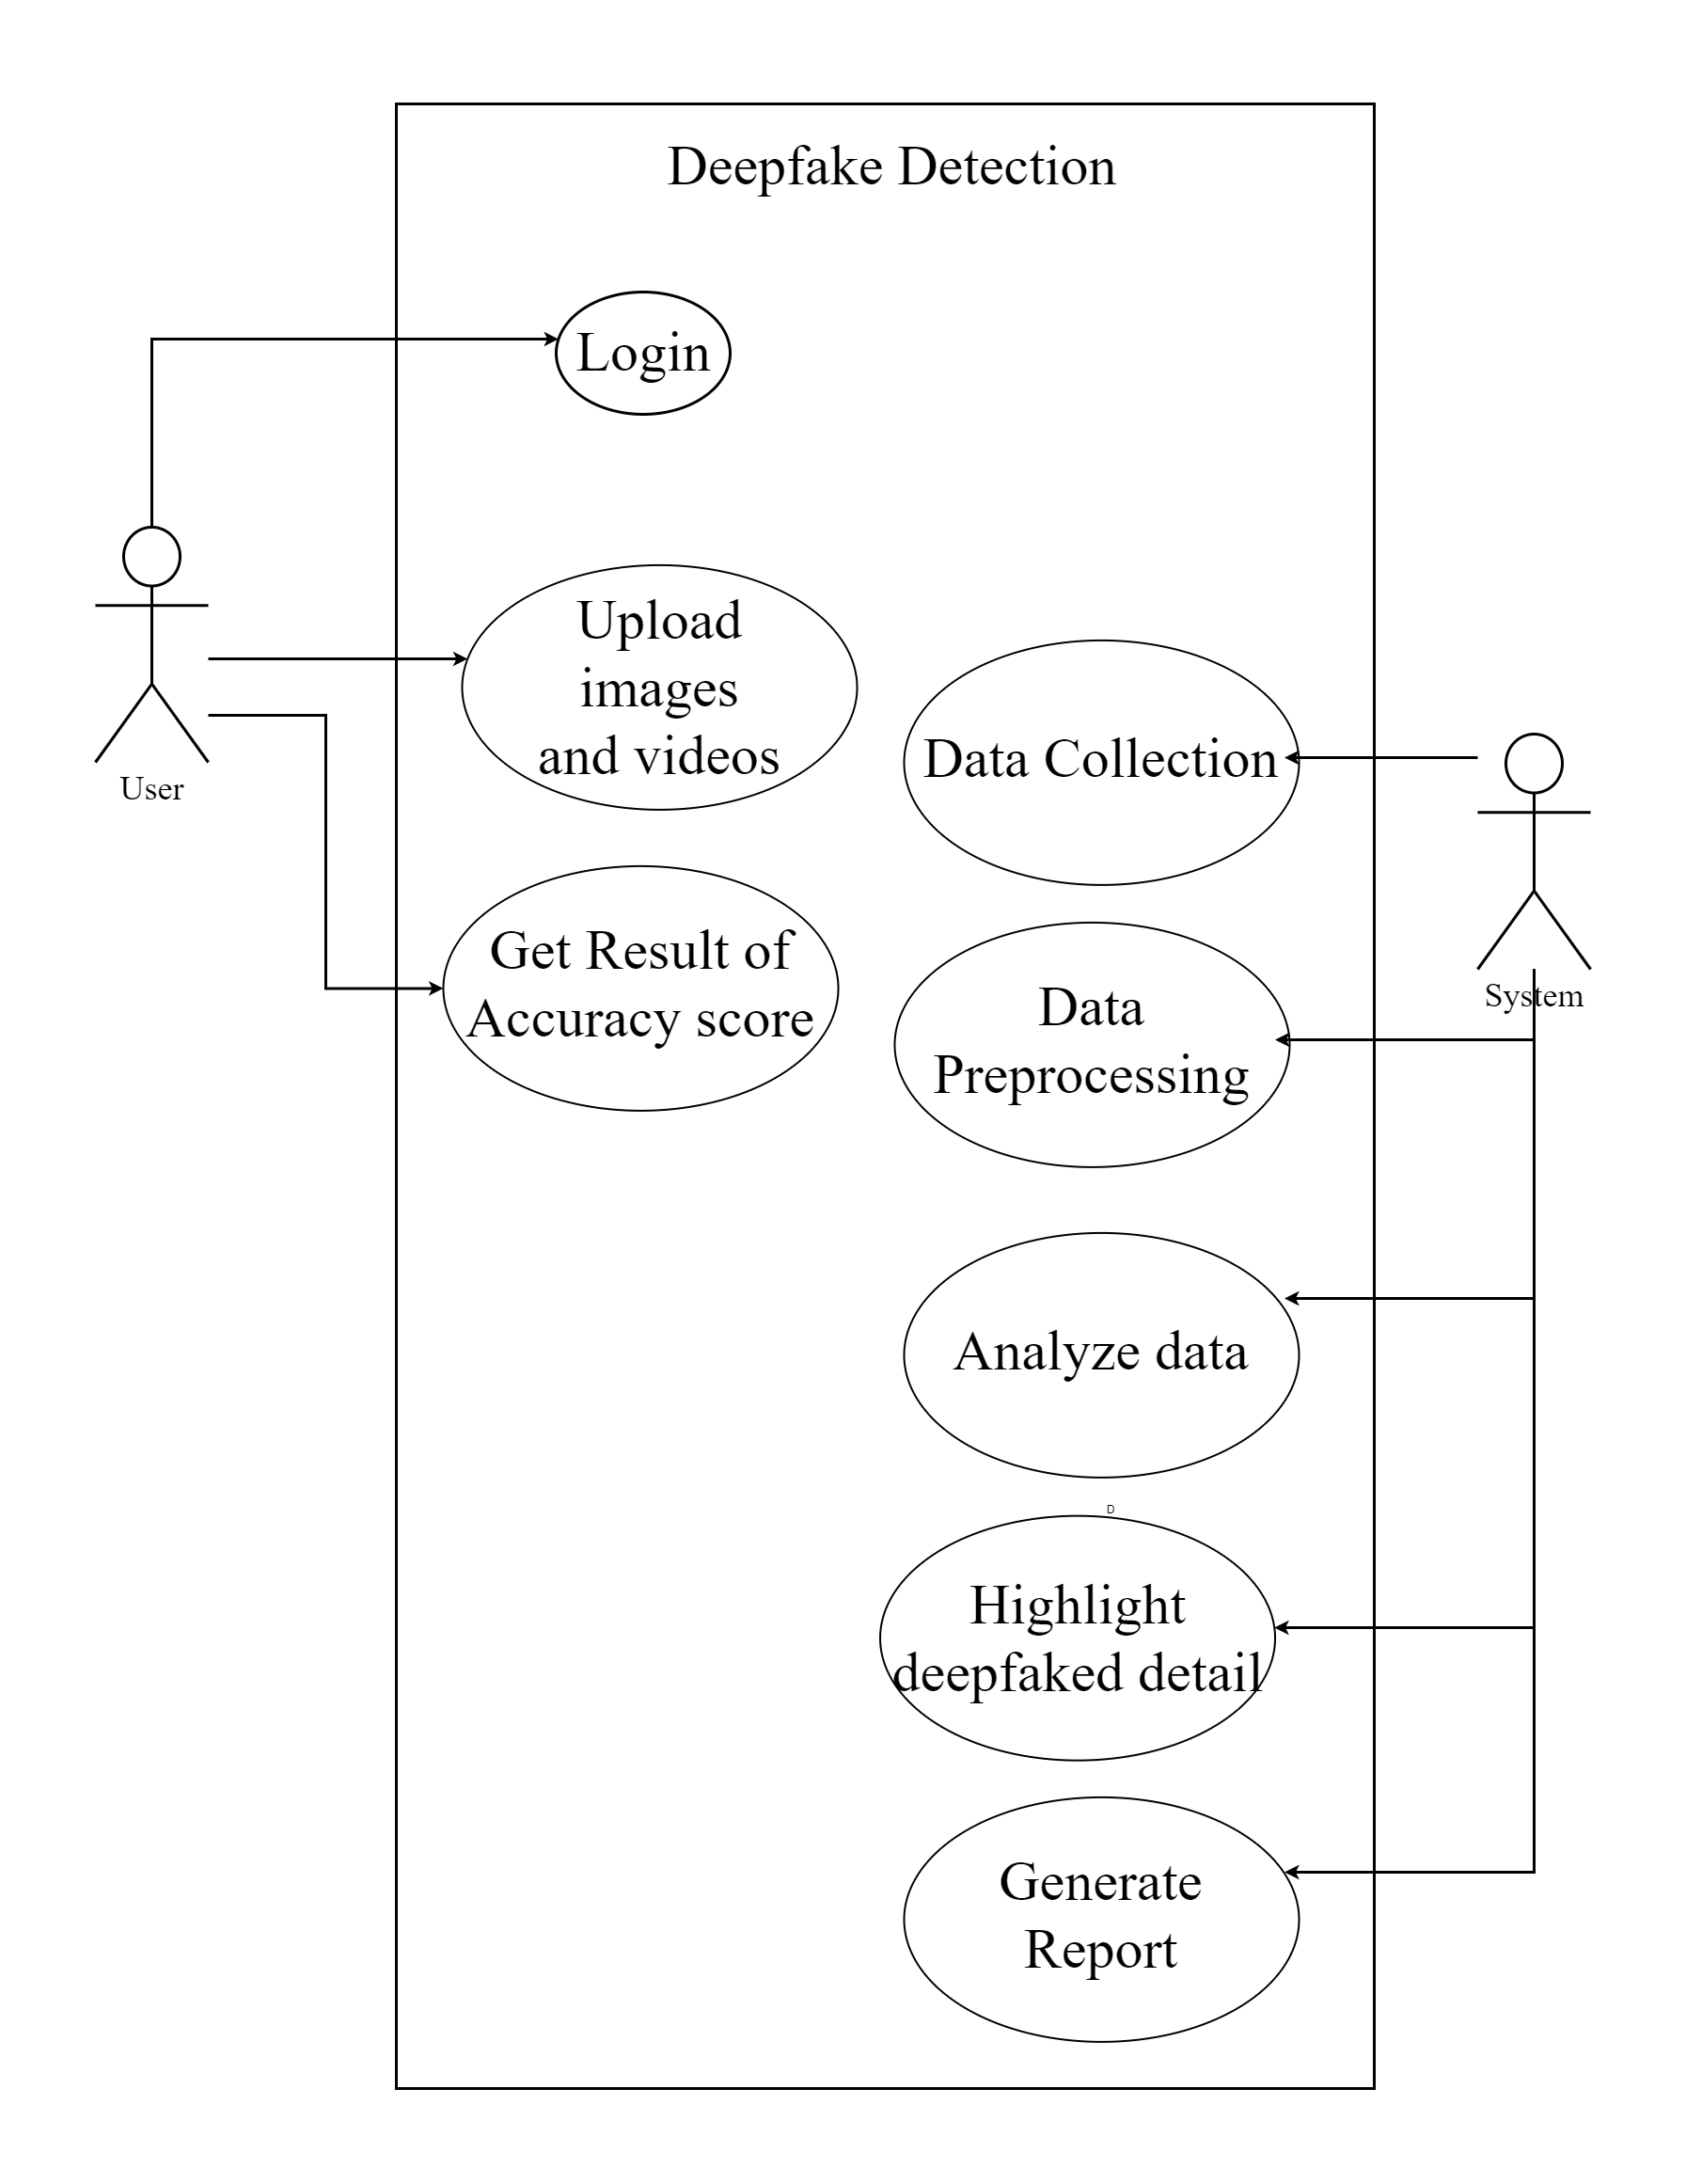
\includegraphics[width= 5.5in ]{img/usecasediagram.drawio.png}
    \caption{{Use Case Diagram}}
\end{figure}
\justify
The use case diagram for our system illustrates various interactions and roles of the system's users. The primary actors involved are the "User" and the "System." The User interacts with the system by initiating the deepfake detection process, either by uploading a video or an image. The User can also access the system to view the detection results. On the other hand, the System is responsible for managing the system, including user authentication, system configuration, and monitoring the overall functionality. The use case diagram shows the main use cases, such as "Upload Media," "Detect Deepfake," and "View Results," which represent the key functionalities of the system.
\newpage

\subsection{Sequence Diagram}

\begin{figure}[h]
    \centering
    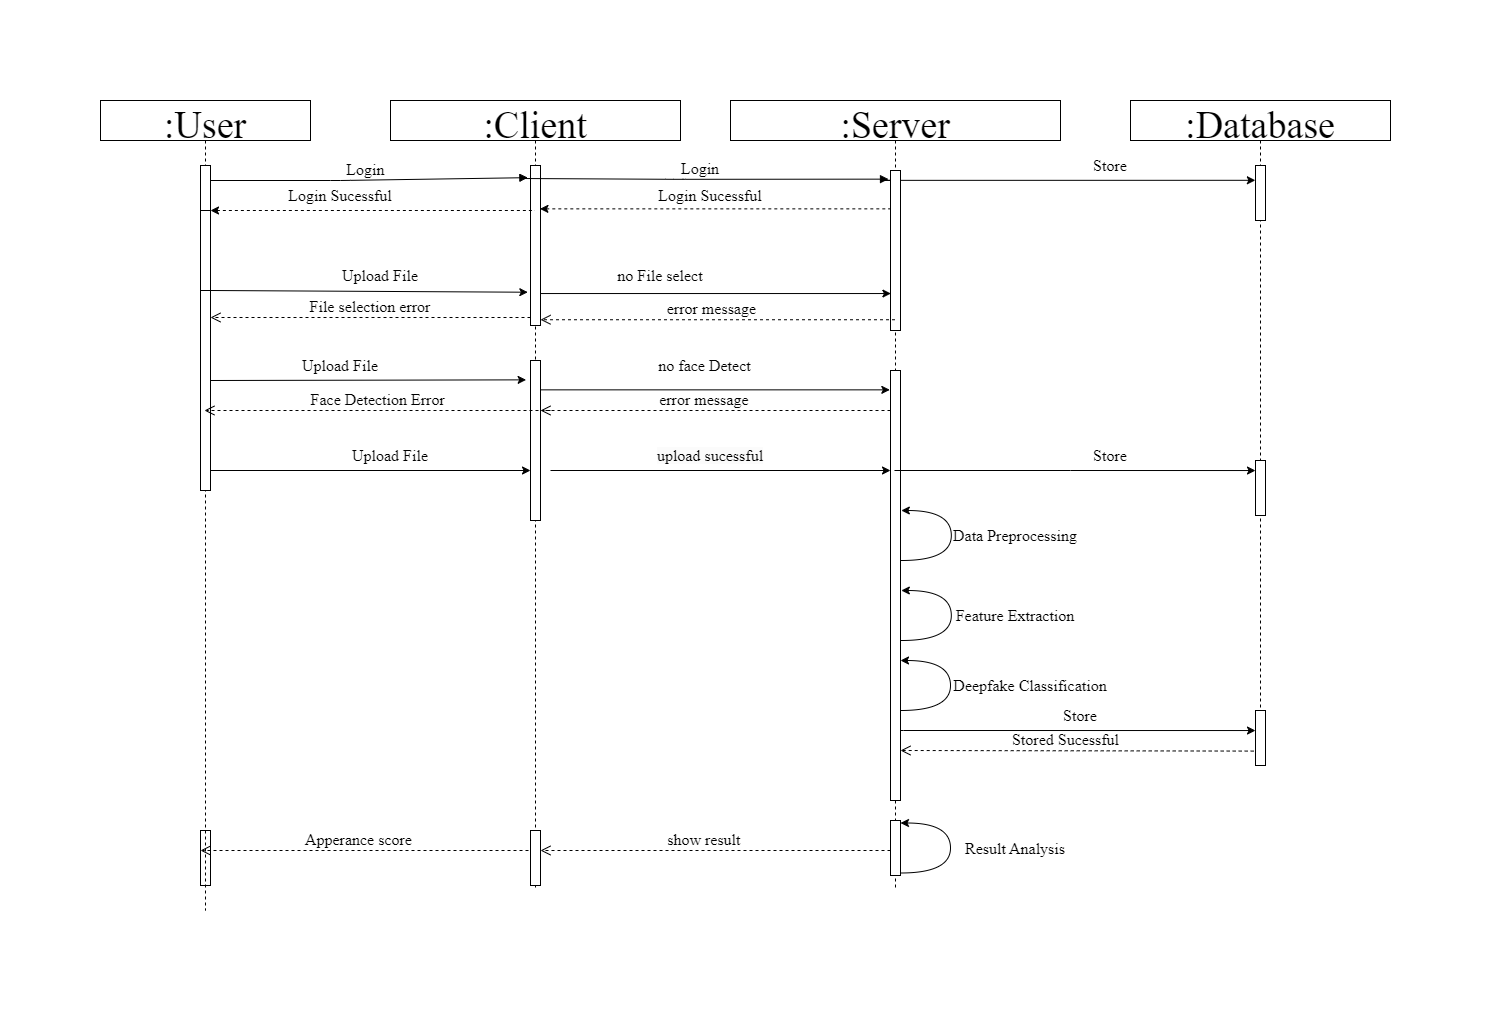
\includegraphics[width=8in]{img/sequencediagram.drawio.png}
    \caption{\textit{Sequence Diagram}}
\end{figure}

\justify
The sequence diagram shows that the user initiates the process by accessing the system and providing their login credentials. The Server checks the login credentials and verifies the user's identity. Once authenticated, the user proceeds to upload a file containing the video or image to be analyzed for deepfakes. Then face detection algorithms are used to detect and extract faces from the uploaded media. This collected data undergoes further processing, including resizing and normalization, to prepare it for deep learning modeling. Finally, the processed data is fed into the deep learning model, which analyzes the features and patterns to classify the media as either real or fake.



\subsection{Dataflow Diagram}
\begin{figure}[h]
    \centering
    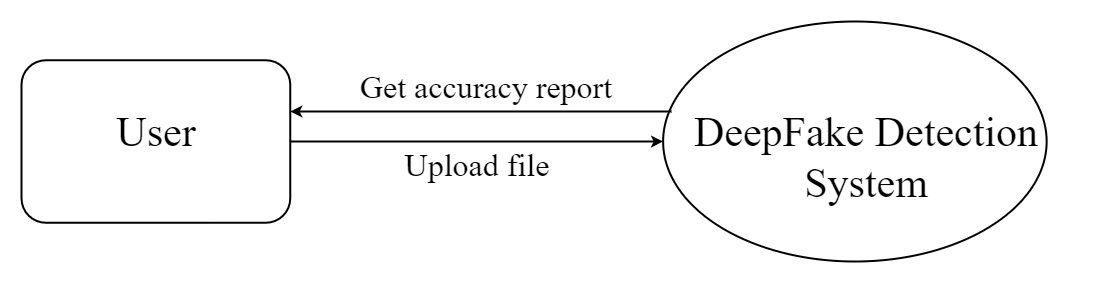
\includegraphics[width= 4in ]{img/level0dfd.drawio.png}
    \caption{\textit{Level 0 DFD}}
\end{figure}

\justify
DFD level – 0 indicates the basic flow of data in the system.
\begin{itemize}
    \item User: User input to the system is uploading video.
    \item System: In system it shows all the details of the Video and output shows the fake video or not. \\
          and output flow
\end{itemize}
Hence, the data flow diagram indicates the visualization of system with its input feed to the system by User.\\
\begin{figure}[h]
    \centering
    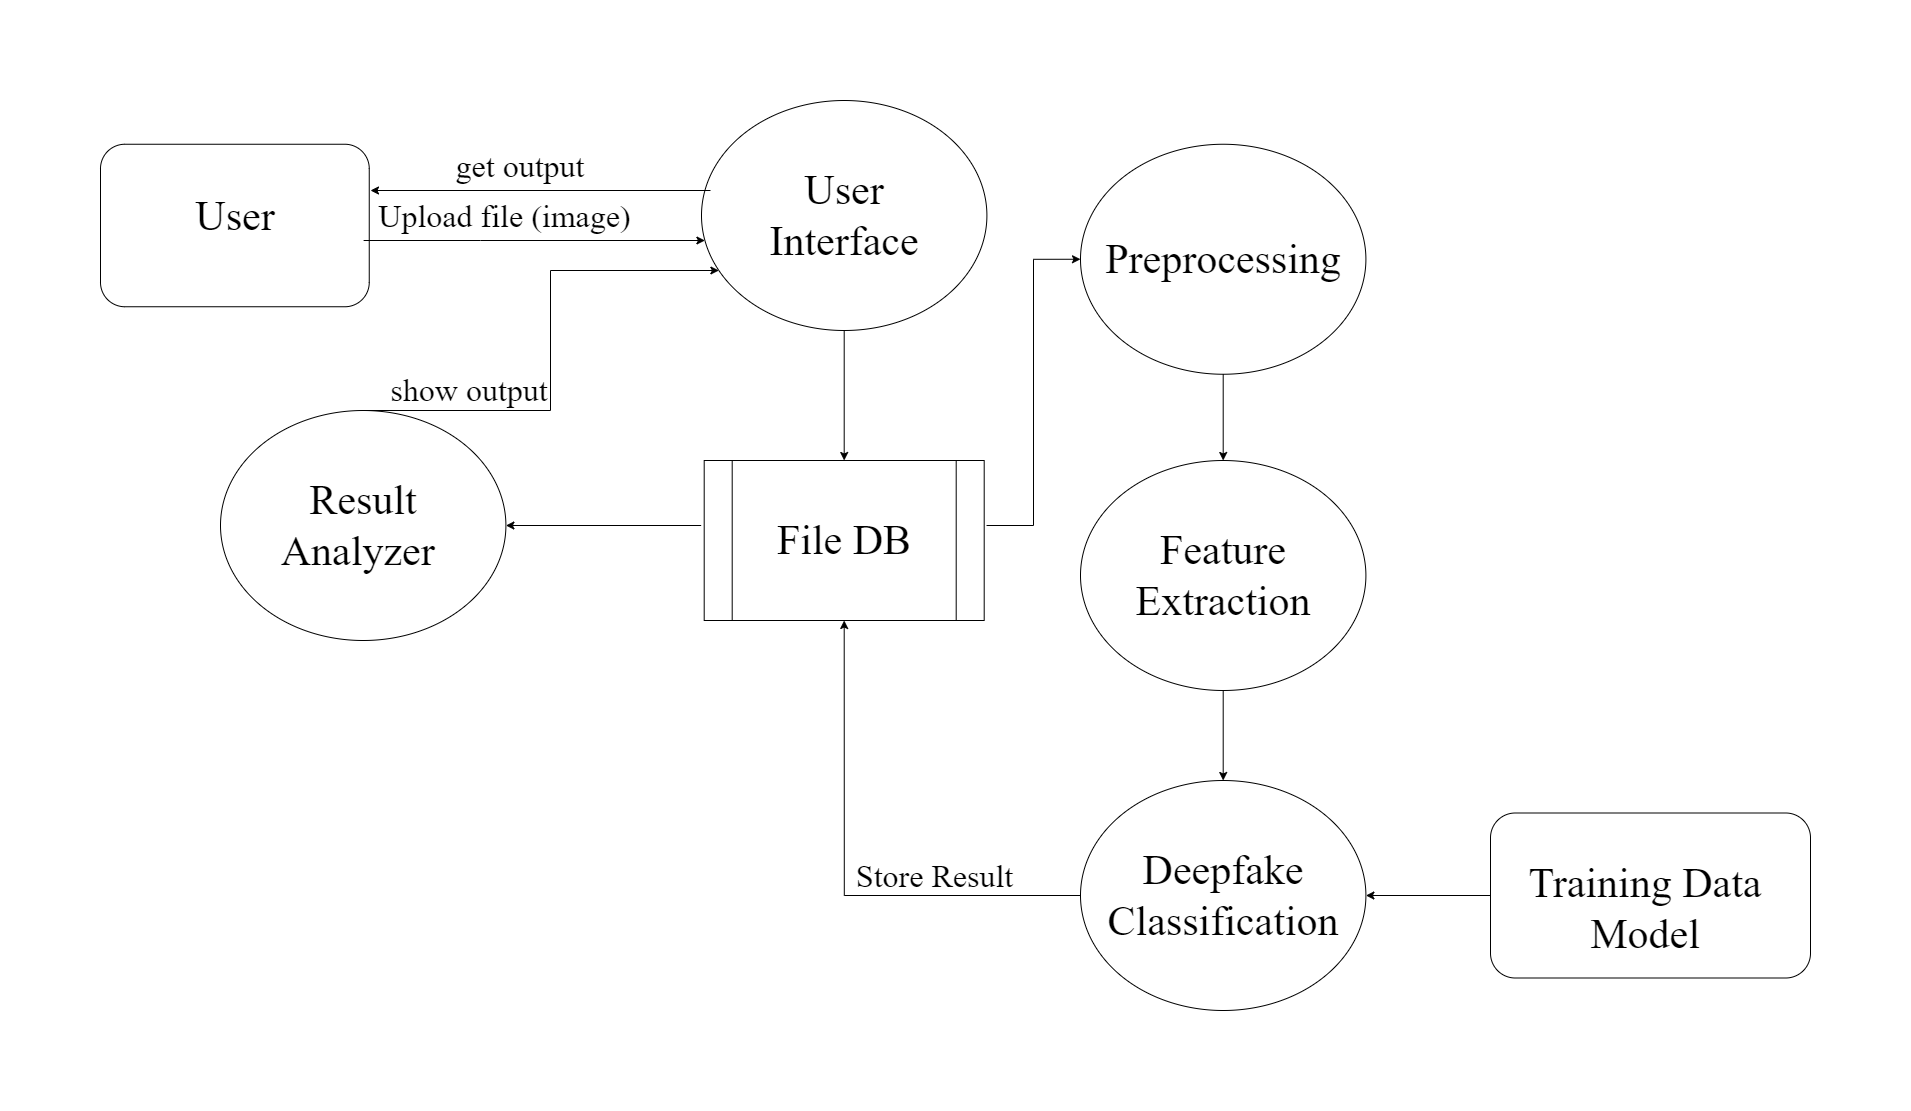
\includegraphics[width= 6in ]{img/level1dfd.drawio.png}
    \caption{\textit{Level 1 DFD}}
\end{figure}
\justify
DFD Level – 1 gives more in and out information of the system.Where system gives detailed information of the procedure taking place.


\subsection{Class Diagram}
\begin{figure}[h]
    \centering
    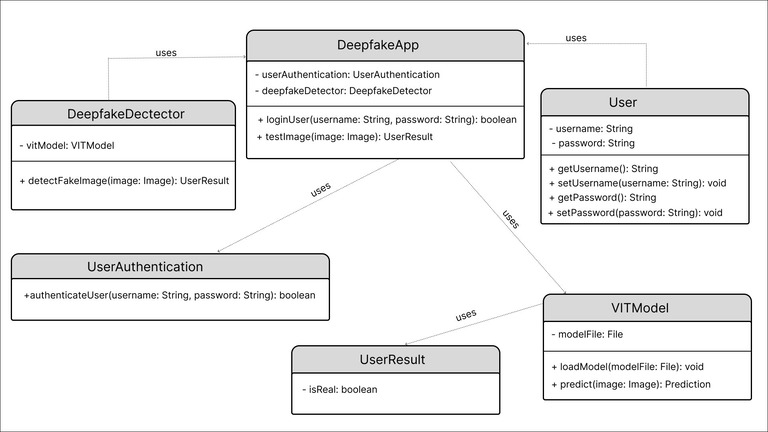
\includegraphics[width=6in,height=6in]{img/classdiagramfig.jpg}
    \caption{\textit{Class Diagram}}
\end{figure}
\justify


\subsection{Activity Diagram}
\begin{figure}[h]
    \centering
    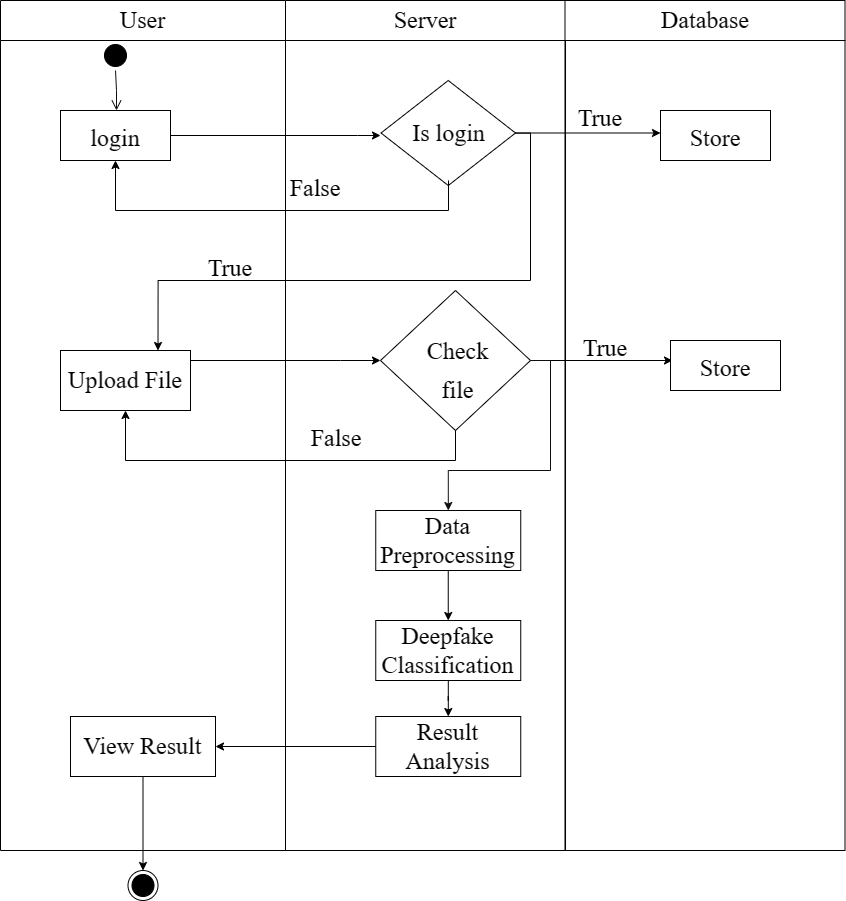
\includegraphics[height=6.5in,width= 6in ]{img/activity diagram.drawio.png}
    \caption{Sequence Diagram}
\end{figure}
\justify
The sequence diagram shows that the user initiates the process by accessing the system and providing their login credentials. The Server checks the login credentials and verifies the user's identity. Once authenticated, the user proceeds to upload a file containing the video or image to be analyzed for deepfakes.Then face detection algorithms is used to detect and extract faces from the uploaded media. This collected data undergoes further processing, including resizing and normalization, to prepare it for deep learning modeling. Finally, the processed data is fed into the deep learning model, which analyzes the features and patterns to classify the media as either real or fake.

\newpage



% 

\section{METHODOLOGY}
\subsection{Software Development Life Cycle}
\justify
Agile method of Software Development uses iterative approach. Agile method cycles
among Planning, Requirement Analysis, Designing, Development and Testing stages.
These cycle is called sprints. Each sprints are considered as a miniature project on itself.
Using this method allowed us to update various parts of project at any point of project
development. In this model an iterative approach was taken where working software
was delivered after each iteration some new features is added to main system. It works
in incremental and iterative approach. Agile model mainly focuses on customer
collaborations, on individuals and iterations and welcomes changes at anytime in
SDLC process. We prefer to use agile model in this system as it helps in developing
realistic systems and promotes teamwork during software development. Also system is
easy to manage and it can accommodate new changes at any stages of software
development phase. \\
\vspace{0.2 in}
% \begin{figure}[h]
%     \centering
%     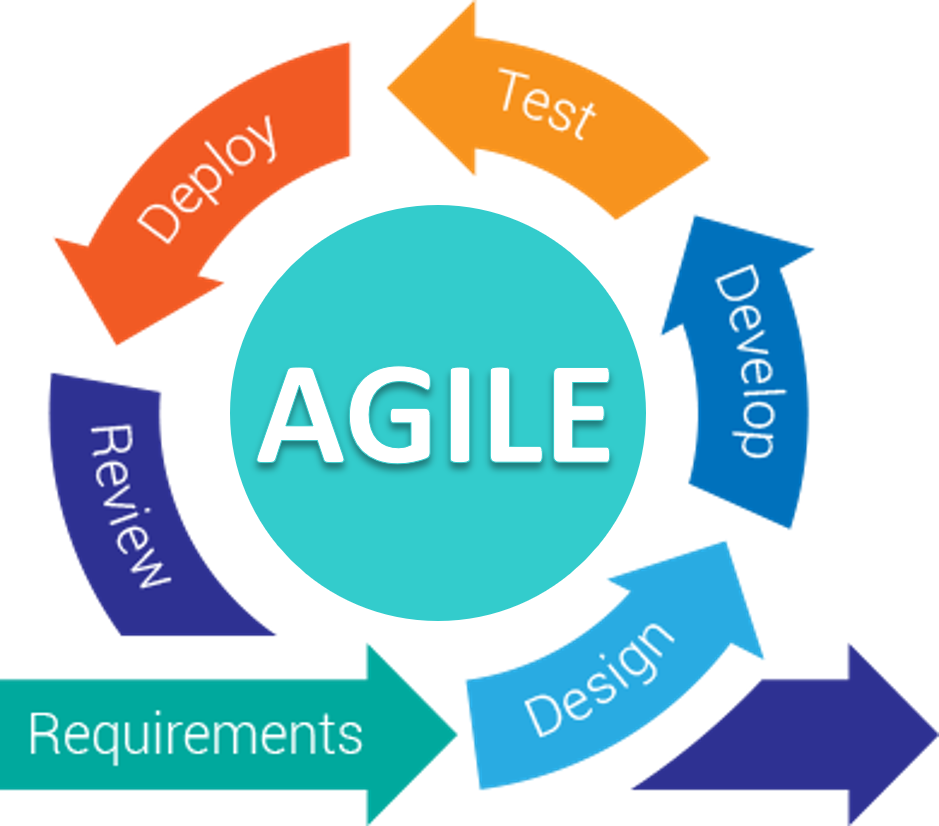
\includegraphics[width= 3in ]{agile.png}
%     \caption{Agile Model}
% \end{figure}

\subsection{Deepfake}
Deepfakes are AI-generated videos or images that convincingly replace the likeness of one person with another, often in a realistic and seamless manner. In today's context, deepfakes raise concerns as they can be used to create misleading content, spreading misinformation, and potentially damaging reputations. This technology has become a notable issue in the age of social media, where manipulated visuals can be easily shared.\\

\begin{figure}[htbp]
    \centering
    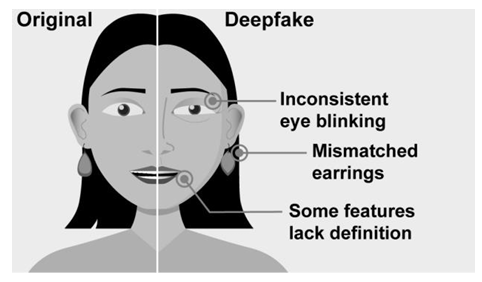
\includegraphics[width=4in]{img/deefakeface.png}
    \caption{\textit{Original vs Deepfakes }}
\end{figure}

Various techniques exist for creating deepfake videos and images, with face swapping and facial manipulation being common methods. Face swapping involves placing the face of one person onto another person's body, while facial manipulation imitates the expressions of one person's face on the face of the target person. Both methods are visually represented in the figure below.\\

\begin{figure}[htbp]
    \centering
    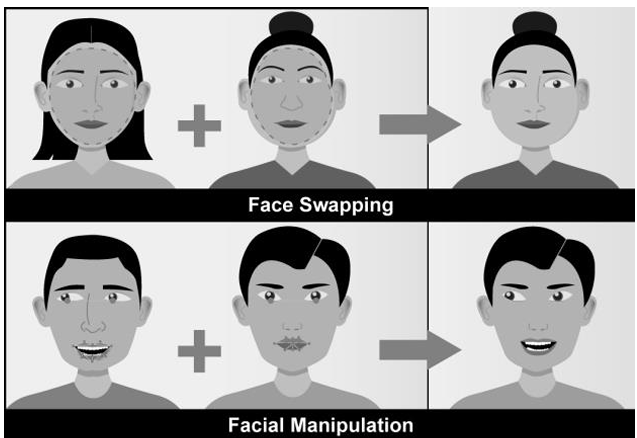
\includegraphics[width=4in]{img/face manipulation.png}
    \caption{\textit{Techniques of Deepfake creation}}
\end{figure}

\newpage




\subsection{Key Features Extraction}

Effective deepfake detection relies on the extraction of specific features from videos or images that can reveal inconsistencies or anomalies introduced by the manipulation process. Various techniques are employed to capture these key features, enabling the development of robust detection models. The following are some of the key features commonly extracted for deepfake detection:

\begin{figure}[htbp]
    \centering
    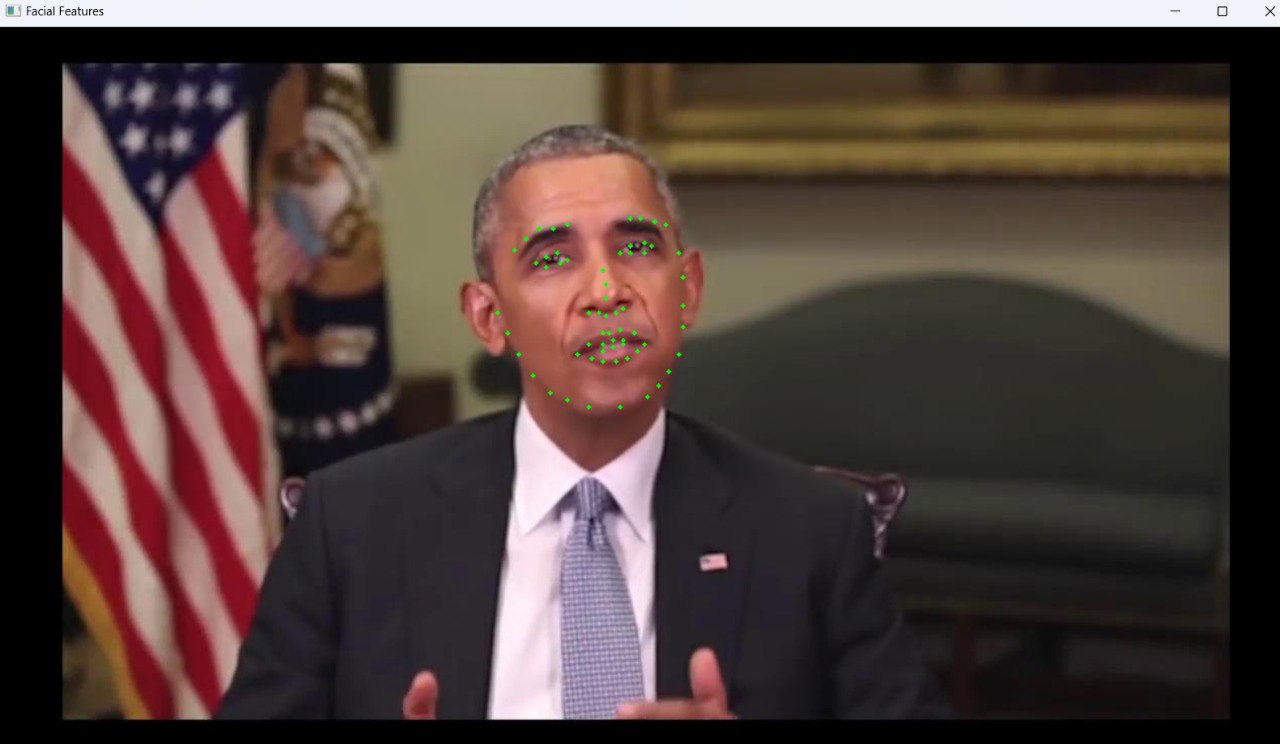
\includegraphics[width= 5in ]{img/featureshighlight.jpg}
    \caption{Facial landmarks extraction from video}
\end{figure}
\subsubsection{Abnormal Patterns}

Deepfake detection methods often look for abnormal patterns that deviate from the expected characteristics of genuine content. These patterns can include unnatural facial expressions, inconsistent facial movements. Detecting such abnormalities through pattern recognition can raise suspicion of manipulation.
\begin{figure}[htbp]
    \centering
    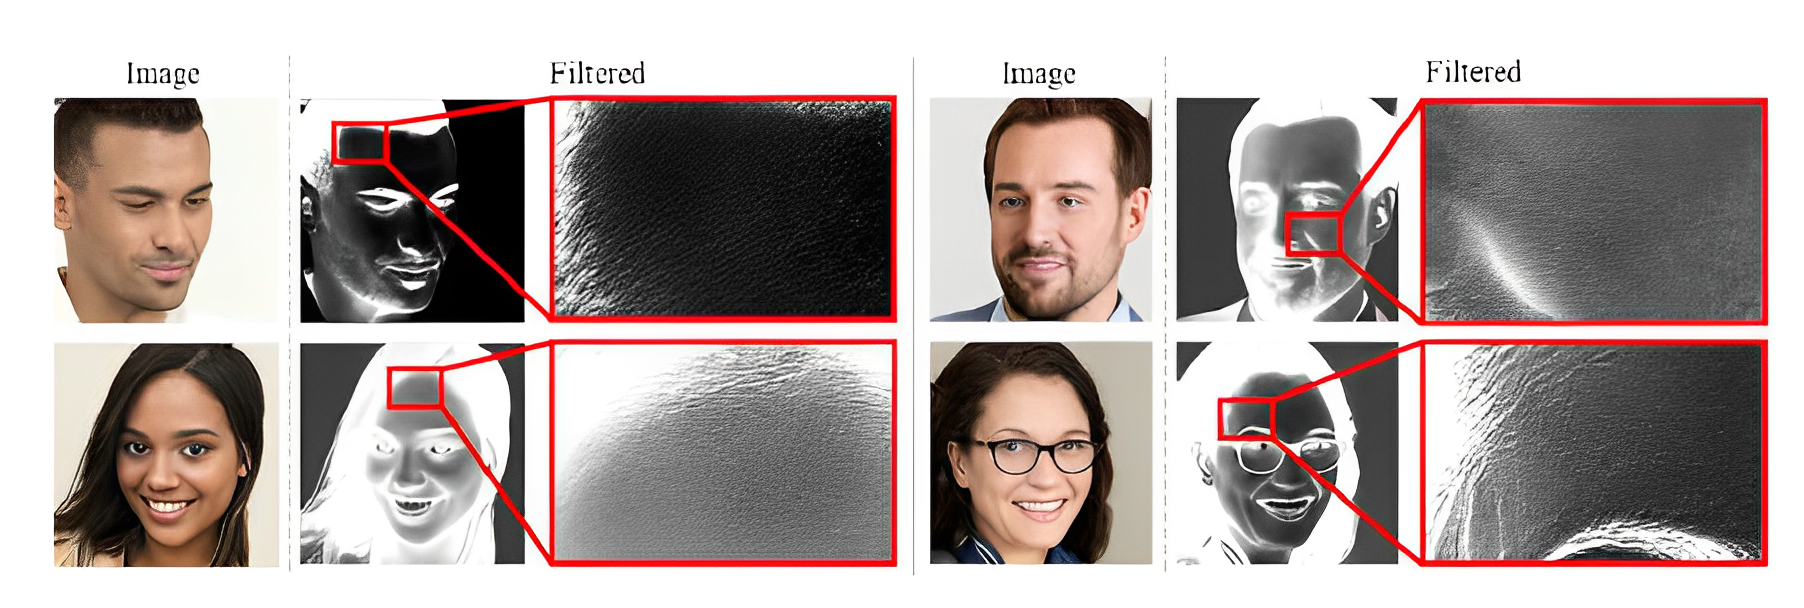
\includegraphics[width=5in]{img/abnormal_pattern.png}
    \caption{Abnormal Patterns}
\end{figure}

\subsubsection{Iris Color and Pupil Boundary}

Iris color and pupil boundary analysis involves examining the color distribution and boundary characteristics of the iris and pupil regions. Variances in iris color or irregularities in pupil shape can indicate potential manipulation. Comparing the extracted features of the iris and pupil between frames can help detect abnormal variations introduced by deepfake techniques.
\begin{figure}[htbp]
    \centering
    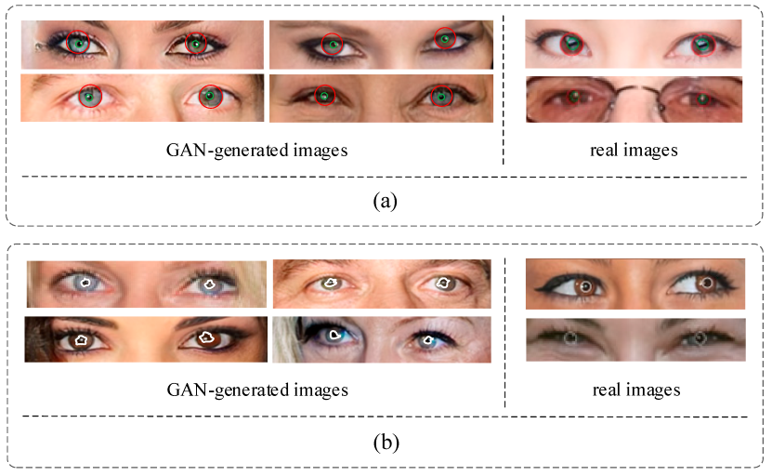
\includegraphics[width=5in]{img/pupil.png}
    \caption{Iris Color and Pupil Boundary}
\end{figure}


\subsubsection{Residual Comparison}

Residual comparison involves analyzing the residuals obtained from subtracting the original image from its manipulated counterpart. By comparing the residuals, artifacts and inconsistencies introduced during the manipulation process can be detected. Unusual patterns or significant deviations between residuals may signify the presence of a deepfake.
\begin{figure}[htbp]
    \centering
    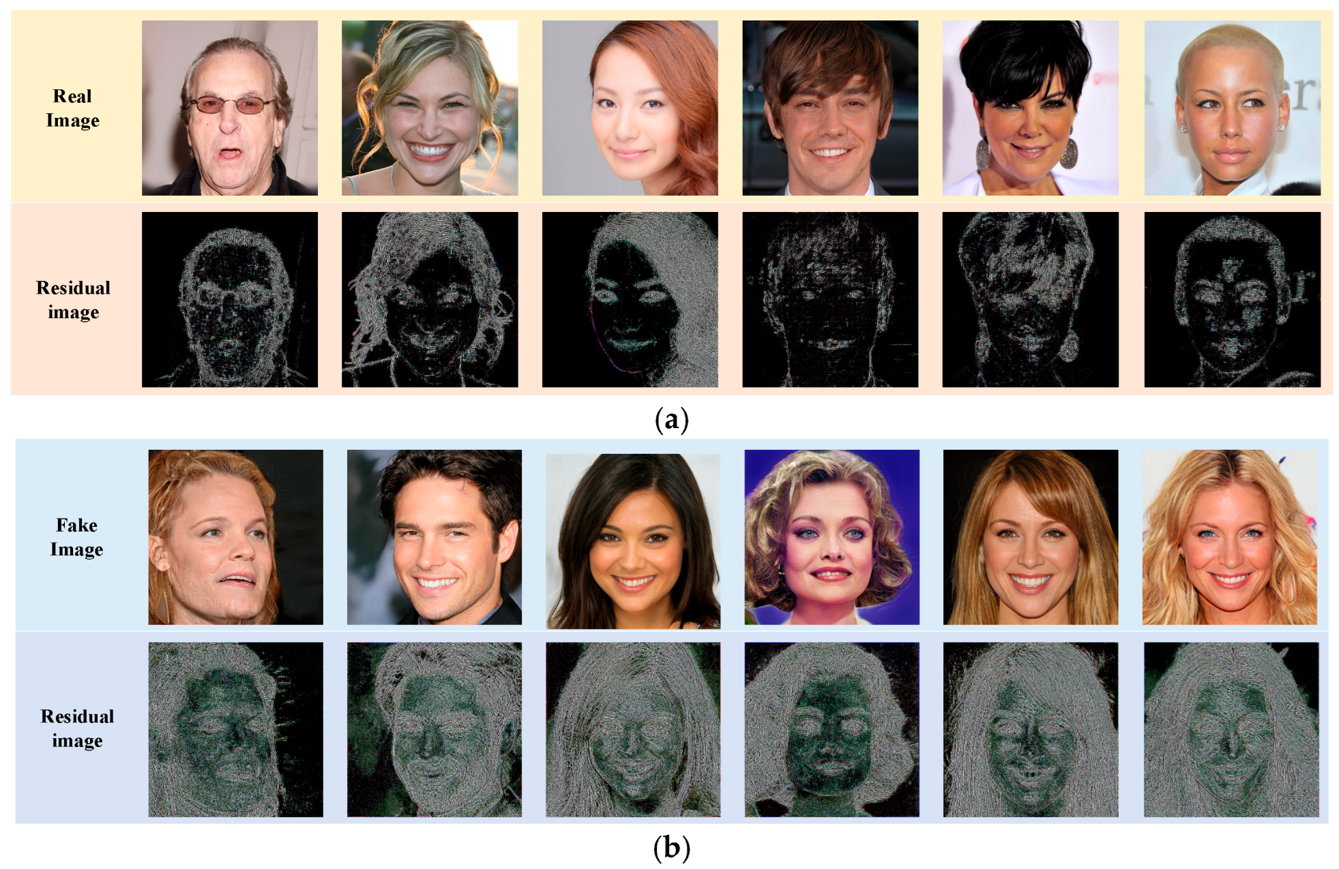
\includegraphics[width=5in]{img/residual.png}
    \caption{Residual}
\end{figure}


\subsubsection{Kernel Density Estimation (KDE) of Color}

Kernel Density Estimation (KDE) involves estimating the probability density function of color values in an image. By applying KDE to different regions of an image, it becomes possible to identify unusual color distributions introduced by deepfake manipulation. Sudden spikes or dips in color density can be indicative of tampering.

\begin{figure}[htbp]
    \centering
    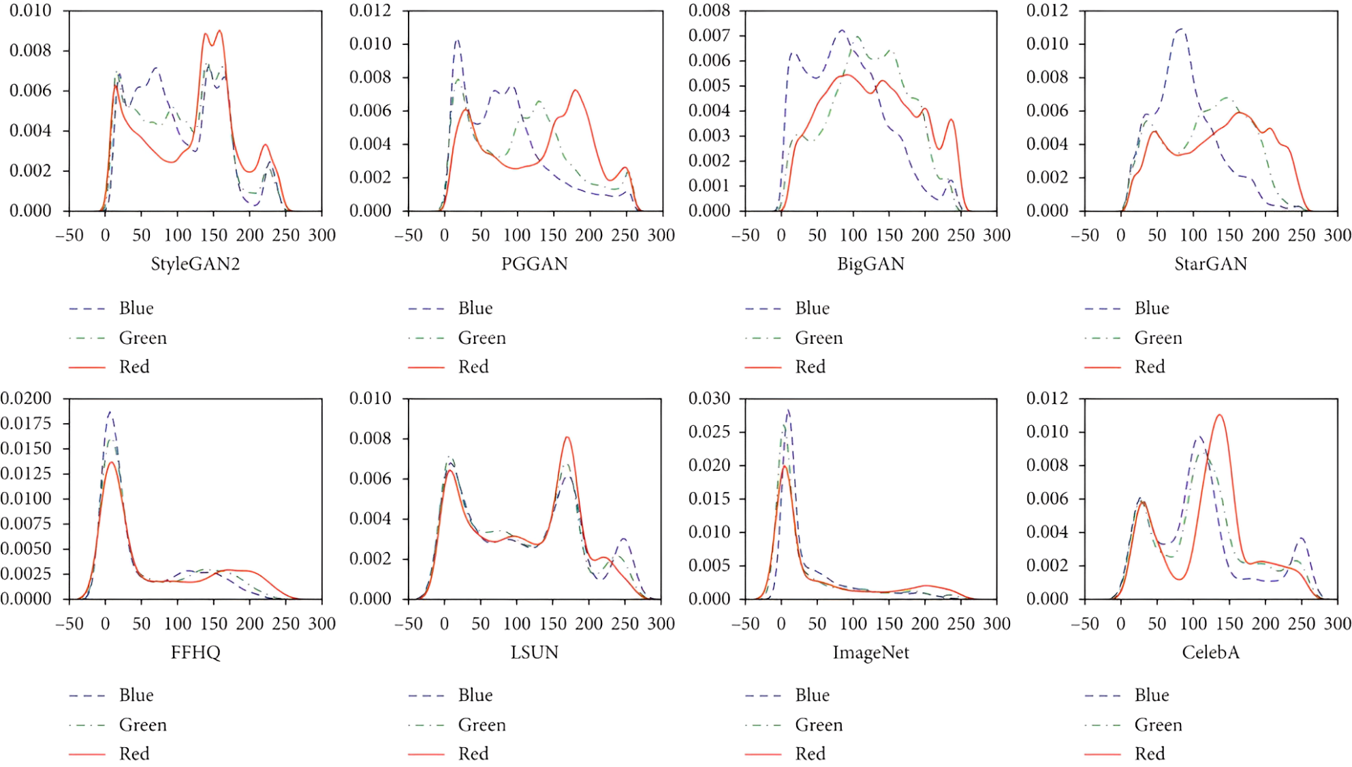
\includegraphics[width=5in]{img/KDE.png}
    \caption{Kernel Density Estimation (KDE) of Color}
\end{figure}

% \subsection{Approach for Deepfake Detection}

For deepfake detection, our approach combines the power of vision transformers with advanced techniques in computer vision. Vision transformers excel in capturing both global and local features within an image, making them suitable for identifying subtle inconsistencies introduced by deepfake manipulation.
\newpage
Our approach involves the following steps:
\vspace{0.2cm}
\begin{enumerate}
    \item \textbf{Dataset Collection}
    \item \textbf{Preprocessing}
    \item \textbf{Vison Transformer Architecture}
    \item \textbf{Training}
    \item \textbf{Evaluation}

\end{enumerate}

% \noindent\textbf{Dataset Collection:} We gather a diverse dataset comprising real and deepfake images. This dataset is crucial for training and evaluating our deepfake detection model.
% \\

% \noindent \textbf{Vision Transformer Architecture:} We chose the Vision Transformer (ViT) architecture due to its ability to process image patches and learn relationships between them using self-attention mechanisms. ViT has shown impressive results in various computer vision tasks, and we adapt it for deepfake detection.
% \\

% \noindent\textbf{Preprocessing:} We preprocess the dataset to extract image patches and resize them to a consistent input size. These patches retain essential information while reducing computational complexity. Additionally, we normalize pixel values to ensure consistent input for the model.
% \\

% \noindent\textbf{Training:} During training, our vision transformer learns to differentiate between real and manipulated images. We use a binary cross-entropy loss function to optimize the model's weights. The self-attention mechanism in the ViT helps the model focus on relevant patches and capture intricate patterns indicative of deepfake manipulation.
% \\

% \noindent\textbf{Evaluation:} We evaluate the model's performance using various metrics such as accuracy, precision, recall, and F1-score. These metrics provide insights into how effectively the model distinguishes between real and deepfake images.
% \\
% \newpage
\subsection{Vision Transformer Architecture}

The Vision Transformer (ViT) is a revolutionary neural network architecture that has significantly advanced the field of computer vision. Introduced as a departure from conventional convolutional neural networks (CNNs), ViT employs a transformer-based model originally designed for natural language processing tasks. This innovative approach involves transforming image data into sequences of tokens, allowing for improved scalability and capturing long-range dependencies in visual information. ViT has demonstrated remarkable success in various computer vision tasks, showcasing its efficiency in image recognition, object detection and segmentation.
\\\\
The Vision Transformer (ViT) architecture comprises the following components:

\begin{figure}[htbp]
    \centering
    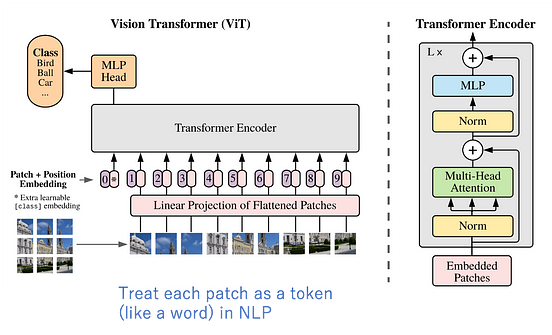
\includegraphics[width=6in]{img/visiontransformer.png}
    \caption{{Vision Transformer Architecture}}
\end{figure}

\item
\subsubsection{Patch Embedding}
The Patch Embedding step in the Vision Transformer architecture involves the following detailed process:
\\

\noindent a. \textbf{Image Patching:} The input image is divided into a grid of non-overlapping patches.\\
Let $\mathbf{X} \in \mathbf{R}^{H \times W \times C}$ represent the original image, where $H$ is the image height, $W$ is the image width, and $C$ is the number of channels (color depth). We partition $\mathbf{X}$ into patches of size $P \times P \times C$, resulting in a tensor $\mathbf{X}_\text{patches} \in \mathbf{R}^{N \times P \times P \times C}$, where $N$ is the total number of patches.
\\

\noindent b. \textbf{Flattening:} Each patch is reshaped into a vector using a flatten operation. The flattened patches are denoted as $\mathbf{X}_\text{flat} \in \mathbf{R}^{N \times (P \times P \times C)}$.
\\

\noindent c. \textbf{Linear Projection:} The flattened patches are projected into a lower-dimensional space using a learnable linear transformation. Let $\mathbf{W}_\text{proj} \in \mathbf{R}^{(P \times P \times C) \times D_\text{proj}}$ be the projection matrix, where $D_\text{proj}$ is the dimension of the projected space. The projected patch embeddings are computed as $\mathbf{E} = \mathbf{X}_\text{flat} \cdot \mathbf{W}_\text{proj} \in \mathbf{R}^{N \times D_\text{proj}}$.
\\

\noindent d. \textbf{Positional Encoding:} To provide spatial information to the transformer model, positional encodings are added to the patch embeddings. Each patch embedding is enhanced with a positional encoding vector $\mathbf{P} \in \mathbf{R}^{N \times D_\text{proj}}$. The final patch embeddings with positional information are given by $\mathbf{E}_\text{pos} = \mathbf{E} + \mathbf{P}$.

\noindent Mathematically, the above steps can be summarized as follows:

\begin{align}
    \mathbf{X}_\text{patches} & = \text{ImagePatching}(\mathbf{X}),                    \\
    \mathbf{X}_\text{flat}    & = \text{Flatten}(\mathbf{X}_\text{patches}),           \\
    \mathbf{E}                & = \mathbf{X}_\text{flat} \cdot \mathbf{W}_\text{proj}, \\
    \mathbf{E}_\text{pos}     & = \mathbf{E} + \mathbf{P}.
\end{align}

The resulting patch embeddings with positional information, $\mathbf{E}_\text{pos}$, are then used as input for the subsequent stages of the Vision Transformer architecture.


\begin{figure}[htbp]
    \centering
    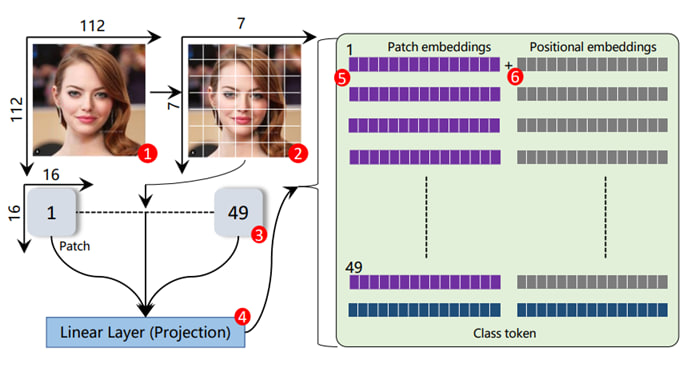
\includegraphics[width=6in]{img/patchembedding.jpg}
    \caption{{Patch Embedding}}
\end{figure}

\subsubsection{Transformer Encoder}
The patch embeddings are then processed through a stack of transformer encoder layers. Each of these layers consists of two main components: multi-head self-attention and feedforward neural networks.
\\


\noindent \textbf{a. Multi-head self-attention:} This mechanism allows the model to consider relationships between different patches, both locally and globally. It assigns different attention weights to different patches based on their relevance to each other, enabling the model to capture long-range dependencies and relationships within the image. \\
\\
\noindent \textbf{Standard qkv Self-Attention (SA)}:
For an input sequence $z \in \mathbf{R}^{N \times D}$ (with $N$ elements, each having a $D$-dimensional feature vector), we compute a weighted sum over all values $v$ in the sequence. The attention weights $A_{ij}$ are determined based on the similarity between elements of the sequence and their corresponding query $q_i$ and key $k_j$ representations.
\begin{align}
    [q, k, v]    & = zU_{qkv}, \quad U_{qkv} \in \mathbf{R}^{D \times 3Dh} \label{eq:qkv}                                               \\
    A            & = \text{softmax}\left(\frac{qk^T}{\sqrt{Dh}}\right), \quad A \in \mathbf{R}^{N \times N} \label{eq:attentionweights} \\
    \text{SA}(z) & = Av \label{eq:selfattention}
\end{align}
\\
MSA extends SA by running $k$ self-attention operations (heads) in parallel and then concatenating their outputs. To ensure consistent computation and parameter complexity, the dimension $Dh$ (from Eq. 5) is usually set to $D/k$.
\begin{align}
    \text{MSA}(z) & = [SA_1(z); SA_2(z); \ldots ; SA_k(z)], \quad U_{msa} \in \mathbf{R}^{k \cdot Dh \times D} \label{eq:multiheadselfattention}
\end{align}

\begin{figure}[htbp]
    \centering
    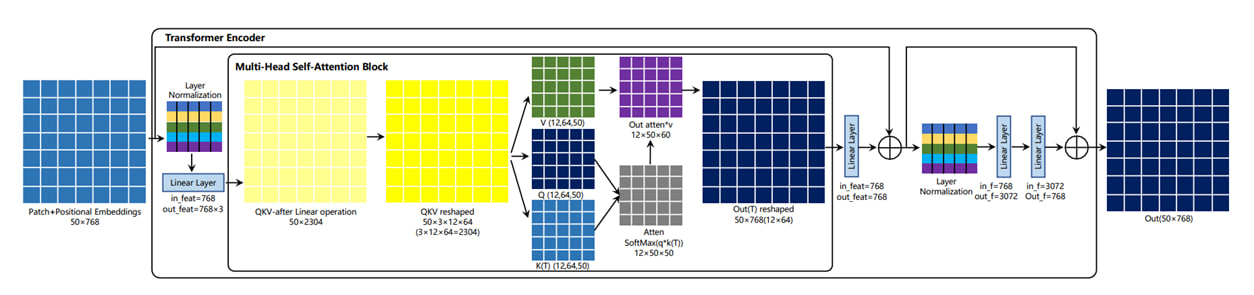
\includegraphics[width=6in]{img/encoderdetails.jpg}
    \caption{{Transformer Encoder}}
\end{figure}

\noindent \textbf{b. Feedforward neural networks:} After the attention mechanism, the data passes through feedforward neural networks, which process and transform the information further, helping the Vision Transformer model learn intricate features and patterns in the image data.

\noindent Feedforward neural networks consist of multiple layers, including fully connected (dense) layers followed by non-linear activation functions. Let's denote the input to the feedforward neural network as $\mathbf{x} \in \mathbf{R}^{D_{\text{FFN}}}$, where $D_{\text{FFN}}$ is the dimension of the input features.
\\

\noindent The transformation in each layer of the feedforward neural network can be represented as follows:

\begin{align}
    \mathbf{h}^{(l+1)} & = \text{GELU}\left(\mathbf{W}^{(l)} \mathbf{h}^{(l)} + \mathbf{b}^{(l)}\right) \label{eq:feedforward}
\end{align}

\noindent where $\mathbf{h}^{(l)}$ is the output of the $l$-th layer, $\mathbf{W}^{(l)}$ is the weight matrix, $\mathbf{b}^{(l)}$ is the bias vector, and $\text{GELU}(\cdot)$ is the Gaussian Error Linear Unit activation function.
\\

\noindent The feedforward neural networks in the Vision Transformer's transformer encoder process each patch embedding independently through these layers, capturing complex patterns and relationships within the data.

\noindent After the final feedforward layer, the resulting representations are concatenated and used as the output of the transformer encoder for further processing or downstream tasks, making the Vision Transformer architecture a powerful tool for image analysis and understanding.


\subsubsection{Classification Head}
The Classification Head is the final component of the Vision Transformer architecture, responsible for making predictions based on the learned features and patterns from the transformer encoder. It performs classification tasks, such as determining whether an image is real or manipulated.
\\

\noindent \textbf{1. Input Preparation:} After going through the transformer layers, the image is divided into patches and transformed into a useful form for the classification head.
\\

\noindent \textbf{2. Pooling Operation:} Think of this as collecting information from all the patches. The model adds up the important parts from each patch and takes the average. This gives a summary of the whole image.
\\

\noindent \textbf{3. Decision Making:} The model uses this summary to decide what the image might be. For example, it could be deciding if an image is real or fake. It does this by comparing the features it has learned to what it has seen during training.
\\

\noindent \textbf{4. Class Prediction:} The model assigns a score to each possible class (like "real" or "manipulated"). It does this by multiplying the summary with a set of numbers that it learned. Then, it uses the softmax function to turn these scores into probabilities. The class with the highest probability is the final prediction.

\subsection{Benefits of Vision Transformer}

The Vision TransformerS (ViT) model has several advantages over many other previous architectures like Convolutional Neural Networks (CNNs) such as:

\begin{itemize}
    \item
          Vision Transformer (ViT) analyzes complete images, ensuring a comprehensive understanding of the global context. This is essential for detecting intricate patterns associated with deepfake manipulation.

    \item It demonstrates efficiency by requiring fewer parameters than traditional Convolutional Neural Networks (CNNs), optimizing memory utilization and training time.

    \item The attention mechanisms in ViT focuses on important and relevant image regions, leading to precision in detecting subtle parameters of deepfake manipulation.

    \item It seamlessly adapts to varied input resolutions, providing flexibility and scalability for effective deepfake detection across diverse datasets.

    \item Vision Transformers process image patches independently, reducing sensitivity to absolute position and increasing robustness against translation and rotation.

    \item Originally designed for image classification, Vision Transformers display adaptability to diverse modals, proving advantageous for multi-modal deepfake detection cases.

\end{itemize}
\newpage

\subsection{Benefits of Vision Transformer}

The Vision TransformerS (ViT) model has several advantages over many other previous architectures like Convolutional Neural Networks (CNNs) such as:

\begin{itemize}
    \item 
    Vision Transformer (ViT) analyzes complete images, ensuring a comprehensive understanding of the global context. This is essential for detecting intricate patterns associated with deepfake manipulation.
    
    \item It demonstrates efficiency by requiring fewer parameters than traditional Convolutional Neural Networks (CNNs), optimizing memory utilization and training time.
    
    \item The attention mechanisms in ViT focuses on relevant image regions, enhancing precision in identifying subtle parameters of deepfake manipulation.
    
    \item ViT seamlessly adapts to varied input resolutions, providing flexibility and scalability for effective deepfake detection across diverse datasets.
    
    \item Vision Transformers process image patches independently, reducing sensitivity to absolute position and increasing robustness against translation and rotation.
    
    \item Originally designed for image classification, Vision Transformers display adaptability to diverse modals, proving advantageous for multi-modal deepfake detection cases.
    
\end{itemize}
\newpage

  
\subsection{Mathematical Modeling}

\subsubsection{Activation Function: Gaussian Error Linear Unit (GELU)}
Activation functions play a crucial role in introducing non-linearity to the feedforward neural network layers. Following the self-attention mechanism's processing of input data, the results traverse through the feedforward neural network. This network involves linear transformations, and activation functions, such as the Gaussian Error Linear Unit (GELU), are applied element-wise. Activation functions enable the network to grasp and approximate complex, non-linear relationships within the data.\\
<<<<<<< HEAD
\\
The Gaussian Error Linear Unit (GELU) stands as an essential activation function within artificial neural networks. Specifically designed to introduce non-linearity to computational processes, GELU offers a seamless approximation to the rectifier linear unit (ReLU) while preserving differentiability.\\
=======

\noindent The Gaussian Error Linear Unit (GELU) stands as an essential activation function within artificial neural networks. Specifically designed to introduce non-linearity to computational processes, GELU offers a seamless approximation to the rectifier linear unit (ReLU) while preserving differentiability.\\
>>>>>>> 0146326a4e58be7d9eb4e75a5d198553f41b641f

\noindent Two formulations of the GELU function are commonly used:

\begin{equation}
    \text{GELU}(x) = 0.5x \left(1 + \tanh\left(\frac{\pi}{2} \cdot \left(x + 0.044715x^3\right)\right)\right) \label{eq:gelu}
\end{equation}

\noindent and

\begin{equation}
    \text{GELU}(x) = \frac{1}{2}x \left(1 + \text{erf}\left(\frac{x}{\sqrt{2}}\right)\right) \label{eq:gelu2}
\end{equation}

\noindent Where:
\begin{itemize}
    \item $x$ is the input to the GELU function.
    \item $\text{erf}(z)$ is the error function.
    \item $\pi$ represents the mathematical constant pi.
    \item $\sqrt{2}$ is the square root of 2.
\end{itemize}

\noindent The GELU activation function is often used in neural network architectures due to its smoothness and differentiability properties, making it suitable for gradient-based optimization during training.

\noindent Additionally, consider the mathematical expression:
\begin{equation}
    P(X = c) \label{eq:probability}
\end{equation}

<<<<<<< HEAD
where $X$ represents a random variable and $c$ is a constant value. This expression is used to represent the probability that the random variable $X$ takes on the value $c$.\\
\\
When no activation function is used in a neural network, the model essentially reduces to a linear regression or a linear transformation. Consequently, the entire neural network collapses into a single linear transformation, regardless of the number of layers. This severely limits the expressive power of the network, as it can only learn linear relationships in the data.\\
=======
\noindent where $X$ represents a random variable and $c$ is a constant value. This expression is used to represent the probability that the random variable $X$ takes on the value $c$.\\

\noindent When no activation function is used in a neural network, the model essentially reduces to a linear regression or a linear transformation. Consequently, the entire neural network collapses into a single linear transformation, regardless of the number of layers. This severely limits the expressive power of the network, as it can only learn linear relationships in the data.\\

\noindent Compared to Rectified Linear Unit (ReLU) and Exponential Linear Unit (ELU), the Gaussian Error Linear Unit (GELU) activation function stands out for its smoothness, handling of negative inputs, and ability to capture complex patterns. ReLU sets all negative values to zero during the forward pass, which can lead to "dead neurons" that never activate and do not contribute to learning. This can result in a loss of information and slower convergence during training. Whereas, ELU largely suffers from vanishing gradient problem.

>>>>>>> 0146326a4e58be7d9eb4e75a5d198553f41b641f
\begin{figure}[htbp]
    \centering
    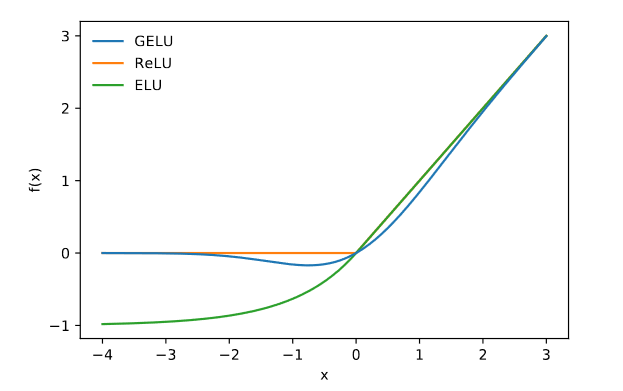
\includegraphics[width=6in]{img/gelu vs relu.png}
    \caption{{GeLU vs ReLU vs ELU graph}}
\end{figure}
\\
Compared to Rectified Linear Unit (ReLU) and Exponential Linear Unit (ELU), the Gaussian Error Linear Unit (GELU) activation function stands out for its smoothness, handling of negative inputs, and ability to capture complex patterns. ReLU sets all negative values to zero during the forward pass, which can lead to "dead neurons" that never activate and do not contribute to learning. This can result in a loss of information and slower convergence during training. Whereas, ELU largely suffers from vanishing gradient problem.


\subsubsection{Loss Function}
The loss function employed in the Vision Transformer (ViT) model is a critical component for training the network and optimizing its performance in image classification tasks. The ViT loss function is designed to measure the disparity between the predicted class probabilities and the ground truth labels.

\paragraph{Cross-Entropy Loss :}
The primary loss utilized in ViT is the Cross-Entropy Loss, also known as categorical cross-entropy. It quantifies the difference between the predicted probability distribution (produced by the softmax activation) and the true distribution of class labels.

\noindent Mathematically, the Cross-Entropy Loss for a single training example is defined as:

\begin{equation}
    L(y, \hat{y}) = -\sum_i y_i \cdot \log(\hat{y}_i) \label{eq:loss_function}
\end{equation}

\noindent where:
\begin{align*}
    y       & \text{ is the ground truth label vector,}                 \\
    \hat{y} & \text{ is the predicted probability distribution vector,} \\
    i       & \text{ iterates over all classes.}
\end{align*}

\subsubsection{Bilinear Interpolation }
Bilinear interpolation is a widely used technique in image processing for estimating pixel values at non-integer coordinates within an image. This method is particularly valuable when scaling or resizing images, offering a smoother transition between neighboring pixels compared to simpler interpolation methods ensuring a smoother and visually appealing transition between pixel values, contributing to improved image quality in various computer graphics and computer vision applications.\\


\noindent \subparagraph{Steps}
\begin{enumerate}
    \item \textbf{Identify Neighboring Pixels:}Given a non-integer coordinate (x, y), locate the four nearest pixels in the image: (x1, y1), (x1, y2), (x2, y1), and (x2, y2), defining a rectangular region

    \item \textbf{Calculate Interpolation Weights:} Compute the horizontal (u) and vertical (v) interpolation weights based on the fractional part of the coordinates (x, y).
          \begin{align}
              u & = x - x_1 \label{eq:u_equation} \\
              v & = y - y_1 \label{eq:v_equation}
          \end{align}


    \item \textbf{Perform Interpolation:} Interpolate along the vertical direction to obtain the interpolated value:
          \begin{align}
              I_{\text{interpolated}} & = (1 - v) \cdot I_{\text{top}} + v \cdot I_{\text{bottom}} \label{eq:interpolated_equation}
          \end{align}


          \text{where:}
          \begin{align}
              I_{\text{top}}    & = (1 - u) \cdot I(x_1, y_1) + u \cdot I(x_2, y_1) \label{eq:itop_equation}    \\
              I_{\text{bottom}} & = (1 - u) \cdot I(x_1, y_2) + u \cdot I(x_2, y_2) \label{eq:ibottom_equation}
          \end{align}


\end{enumerate}
\subsubsection{Layer Normalization}
The Layer Normalization is applied independently to each position (or patch) in the input sequence.Layer Normalization is very similar to Batch normalization but layer normalization is favored because it works independently on each patch of the image sequence, aligning well with ViT's sequential processing.\\

\noindent Given an input tensor $x$ at a particular position, the Layer Normalization is computed using the formula:

\begin{equation}
    \text{LayerNorm}(x) = \frac{x - \text{mean}(x)}{\sqrt{\text{var}(x) + \epsilon}} \cdot \gamma + \beta \label{eq:layer_norm}
\end{equation}


\noindent Here, $\text{mean}(x)$ and $\text{var}(x)$ represent the mean and variance of the input $x$ at that position, and $\gamma$ and $\beta$ are learnable parameters. $\epsilon$ is a small constant for numerical stability.\\

<<<<<<< HEAD
\noindent \textbf{Importance:}Layer Normalization is crucial for stabilizing training by normalizing the activations at each position. It helps mitigate change in the distribution of the input during training, making the model less sensitive to changes in input distribution. This normalization facilitates more stable and efficient training, enabling the model to better capture complex hierarchical features in image data.\\
=======
\noindent \textbf{Importance:}
Layer Normalization is crucial for stabilizing training by normalizing the activations at each position. It helps mitigate change in the distribution of the input during training, making the model less sensitive to changes in input distribution. This normalization facilitates more stable and efficient training, enabling the model to better capture complex hierarchical features in image data.\\
>>>>>>> 0146326a4e58be7d9eb4e75a5d198553f41b641f

\subsubsection{Positional Encoding}
Positional encoding is used Vision Transformer to provide information about the position of tokens in a sequence. Since transformers don't inherently understand the order of tokens, positional encoding helps inject spatial information into the input data.\\

\noindent Formula for 1D positional encoding for a token at position $pos$ in a sequence of length $L$ with embedding dimension $d$:\\

\begin{equation}
    \text{PE}(pos, 2i) = \sin\left(\frac{pos}{10000^{2i/d}}\right) \label{eq:pos_encoding_sin}
\end{equation}

\begin{equation}
    \text{PE}(pos, 2i+1) = \cos\left(\frac{pos}{10000^{2i/d}}\right) \label{eq:pos_encoding_cos}
\end{equation}


\noindent Here, $pos$ is the position, $i$ is the dimension, and $d$ is the embedding dimension. The positional encoding values are added to the original embeddings of the tokens.\\

\noindent In essence, the formula generates unique sinusoidal patterns for each position and dimension, enabling the model to distinguish the order of tokens in the sequence. This helps transformers effectively process sequential data, such as text or images divided into patches.\\

\subsubsection{Softmax Score}
The softmax function is used to convert a vector of real numbers into a probability distribution. In the context of machine learning and neural networks, it is often applied to the raw scores or logits produced by the model. The softmax function ensures that the values in the resulting vector are between 0 and 1 and sum to 1. It's commonly used in the output layer of a classification model to obtain probabilities for each class.\\

<<<<<<< HEAD
\noindent Given an input vector \(z\) with \(K\) elements, the softmax function is calculated as follows:\\

=======
\noindent Given an input vector \(z\) with \(K\) elements, the softmax function is calculated as follows:
>>>>>>> 0146326a4e58be7d9eb4e75a5d198553f41b641f
\begin{equation}
    \text{Softmax}(z)_i = \frac{e^{z_i}}{\sum_{j=1}^{K} e^{z_j}} \label{eq:softmax}
\end{equation}


\noindent Here, \(\text{Softmax}(z)_i\) represents the \(i\)-th element of the resulting softmax vector. \(e\) is the base of the natural logarithm (Euler's number). The numerator is the exponentiation of the \(i\)-th element of \(z\), and the denominator is the sum of the exponentiations of all elements in \(z\).\\

\noindent The softmax operation essentially transforms the input vector into a probability distribution, making it suitable for tasks like multiclass classification where the goal is to assign probabilities to different classes.\\

\subsubsection{Adam Optimizer}

\noindent The Adam optimizer, short for Adaptive Moment Estimation, combines the advantages of adaptive learning rates, momentum optimization, and the Root Mean Square Propagation (RMSProp) algorithm. Adam is known for its efficiency, stability, and adaptability across a variety of neural network architectures and datasets.\\

\noindent Adam excels in handling large datasets with varying or sparse gradients. It dynamically adjusts learning rates for each parameter, enhancing adaptability during training. By integrating momentum and RMSProp techniques, Adam accelerates convergence and prevents local minima.\\

\noindent The Adam optimizer updates model parameters based on the following mathematical expressions:

\begin{enumerate}
    \item \textbf{Initialization:}
          \begin{equation}
              m_0 = 0, \quad v_0 = 0
          \end{equation}

    \item \textbf{Moments computation (for obtaining minimum approximation)}
          \begin{align}
              m_t & = \beta_1 \cdot m_{t-1} + (1 - \beta_1) \cdot g_t   \\
              v_t & = \beta_2 \cdot v_{t-1} + (1 - \beta_2) \cdot g_t^2
          \end{align}

    \item \textbf{Bias Correction:}
          \begin{align}
              \hat{m}_t & = \frac{m_t}{1 - \beta_1^t} \\
              \hat{v}_t & = \frac{v_t}{1 - \beta_2^t}
          \end{align}

    \item \textbf{Update Parameters:}
          \begin{equation}
              \theta_{t+1} = \theta_t - \frac{\eta}{\sqrt{\hat{v}_t} + \epsilon} \cdot \hat{m}_t
          \end{equation}
\end{enumerate}

Where:
\begin{itemize}
    \item \( \eta \) is the learning rate.
    \item \( \beta_1 \) and \( \beta_2 \) control the exponential decay rates for the moment estimates.
    \item \( \epsilon \) is a small constant to prevent division by zero.
\end{itemize}

\noindent These equations describe the adaptive learning rate mechanism and the combination of momentum and RMSProp, for Adams Optimizer.






\subsection{Dataset Collection}

\noindent Our dataset acquisition process involved the following steps:


\subsubsection{Public Datasets}
A significant part of our extensive dataset was thoughtfully put together from openly accessible collections of deepfake and authentic images. We carefully chose these datasets to make our deepfake detection model more diverse and applicable. This approach helps us ensure a strong and thorough training and testing process by making the most of these available resources.

Here's the breakdown of our dataset:
\begin{itemize}
    \item \textbf{Total:} 446,000 samples
    \item \textbf{Trained:} 406,000 samples
    \item \textbf{Tested:} 20,0000 samples
    \item \textbf{Validation:} 20,000 samples
\end{itemize}
Our dataset contains data from well-known public sources, and each of these sources has a specific role in making our deepfake detection system better :

\begin{enumerate}
    \item \textbf{CelebA:} CelebA is a large-scale face attributes dataset with annotations for 40 attributes, commonly used for facial recognition and generative tasks.

    \item \textbf{FFHQ (Flickr-Faces-HQ):} FFHQ is a high-resolution face dataset containing 70,000 images from diverse identities, frequently utilized for training high-quality face generation models. We have used 50,000 images from the datasets.

    \item \textbf{StarGAN:} StarGAN is a dataset for image-to-image translation tasks, facilitating research in image translation, domain adaptation, and style transfer.

    \item \textbf{AttGAN:} AttGAN is a dataset designed for facial attribute manipulation, providing images with annotations for training models in attribute-based image editing.

    \item \textbf{StyleGAN:} StyleGAN is a dataset used with the StyleGAN model, capable of generating diverse and high-quality images, popular for art generation and creative applications.

    \item \textbf{StyleGAN2:} StyleGAN2 is an enhanced version of StyleGAN, producing higher quality and more realistic images, widely used for generative image synthesis.

\end{enumerate}


\subsubsection{Video Conversion}
To include videos in our dataset, we first converted them into individual frames (images) to facilitate compatibility with the vision transformer architecture. This step involved extracting frames at a consistent frame rate from each video, resulting in a sequence of images for each video.
\begin{figure}[htbp]
    \centering
    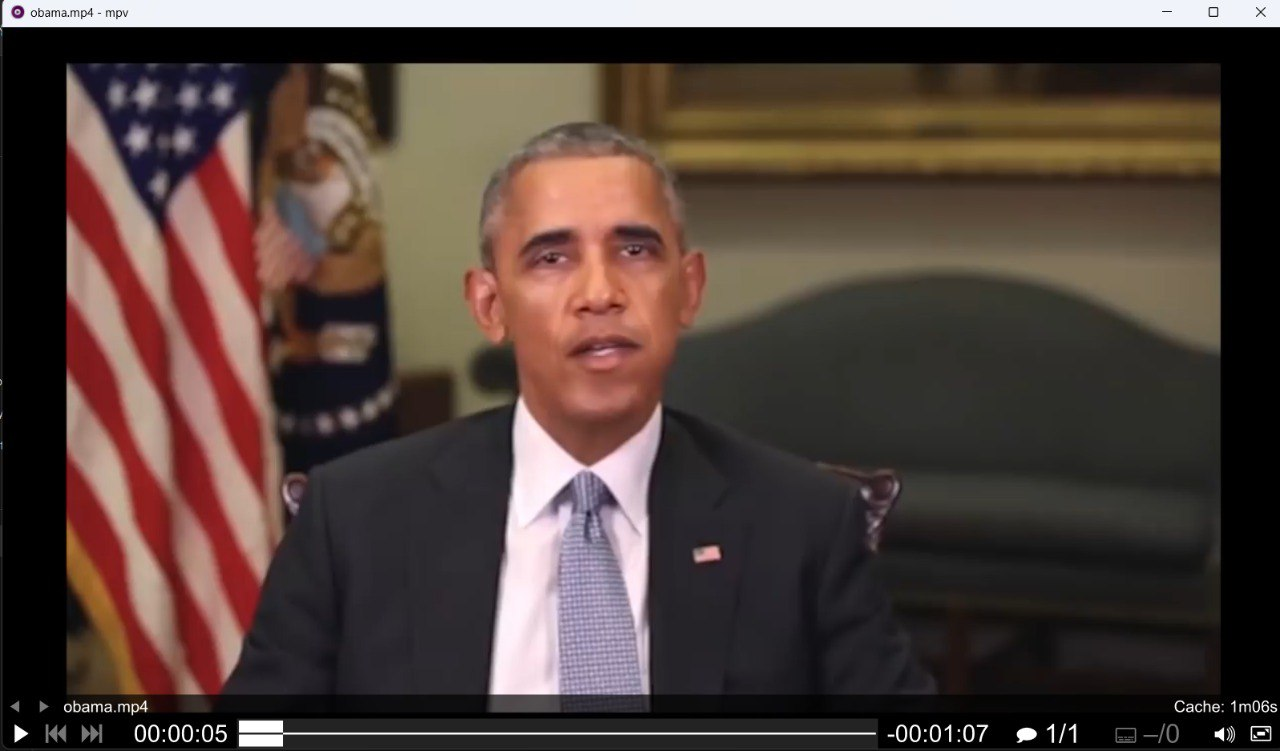
\includegraphics[width= 5in ]{img/framesExtracted.jpg}
    \caption{Video Sample}
\end{figure}
\begin{figure}[ht]
    \centering
    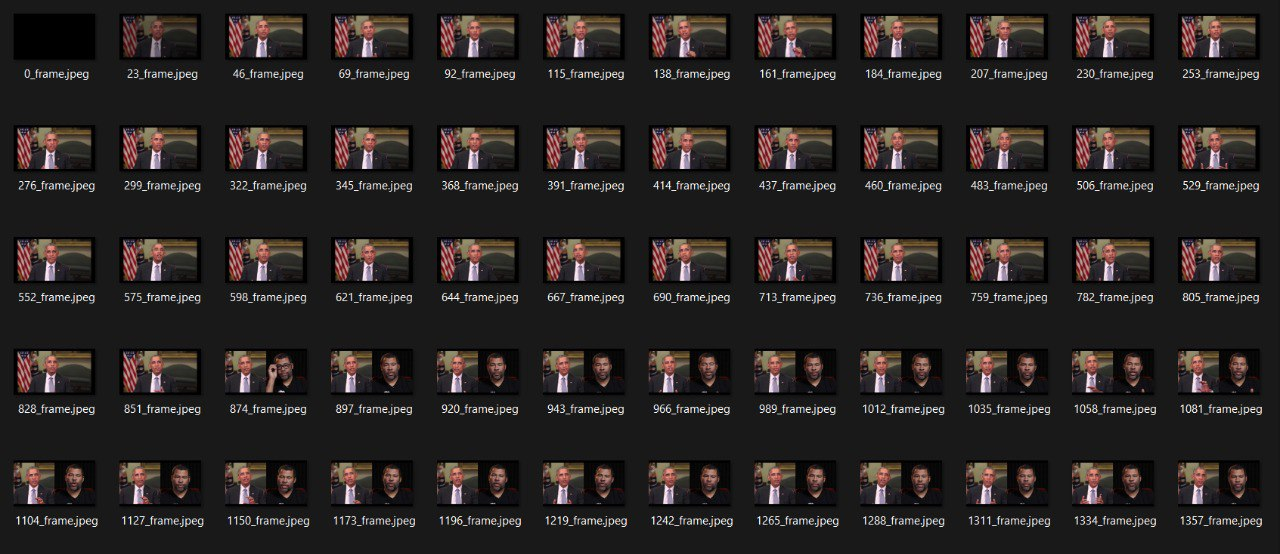
\includegraphics[width= 5in ]{img/frames.jpg}
    \caption{Frames Extracted from video}
\end{figure}

\subsubsection{Frame Selection}
To avoid redundancy and maintain dataset balance, we carefully selected frames from videos to represent various stages of manipulation, expressions, poses, and lighting conditions.

\begin{figure}[htbp]
    \centering
    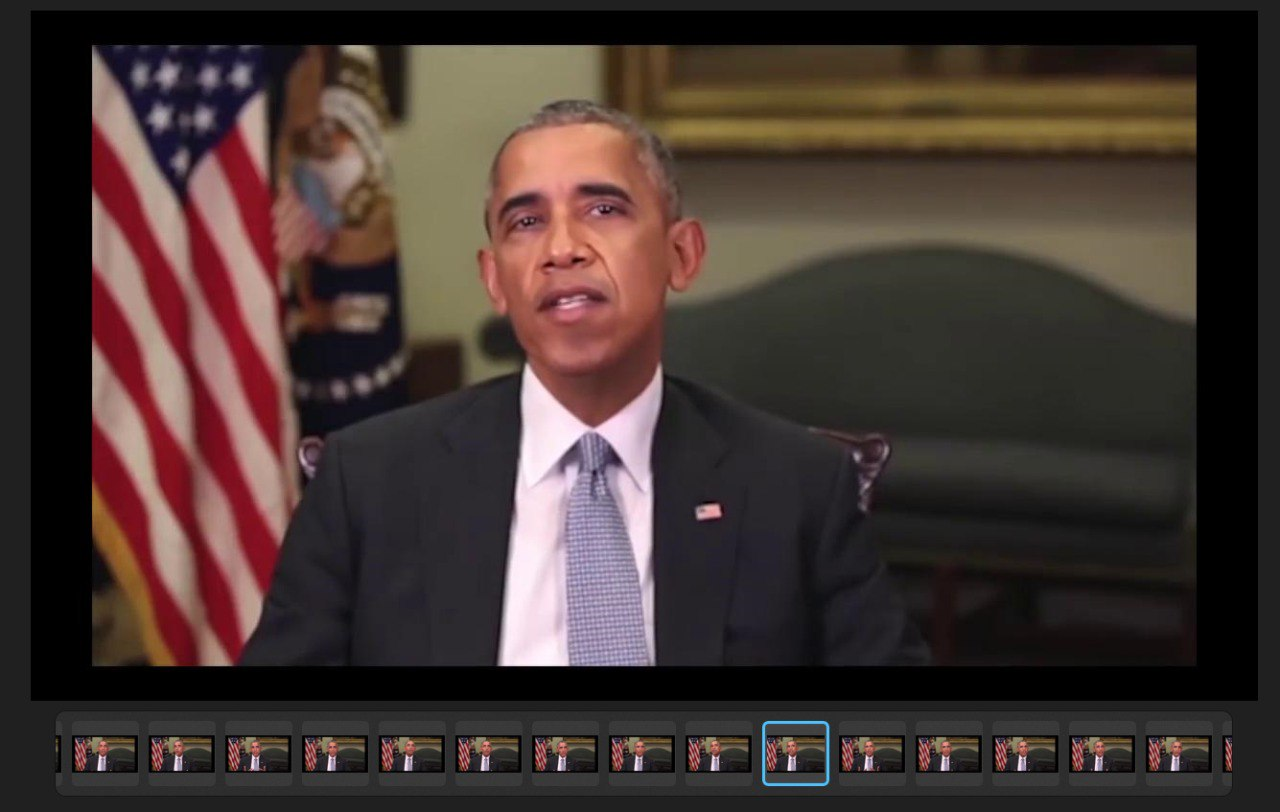
\includegraphics[width= 5in ]{img/frameSelected.jpg}
    \caption{Seleting required frames}
\end{figure}


\subsubsection{Annotation and Labeling}
Each image was labeled as either "real" or "deepfake." Annotations were done manually to ensure accurate labeling for training and evaluation.

\subsection{Algorithm}
The algorithm  for our model is as follows:

\begin{enumerate}
    \item \textbf{Libraries import:}
          \begin{enumerate}
             \item Importing the necessary libraries and modules, including TensorFlow, scikit-learn, and facealignment.
          \end{enumerate}
 
    \item \textbf{Load and Preprocess Data:}
          \begin{enumerate}
             \item Loading the video data using a video processing library.
             \item Extracting the frames from the video.
             \item Applying the face alignment using the \texttt{facealignment} library to ensure consistent face positions.
             \item Resizing each frame to 256x256 using bilinear interpolation.
          \end{enumerate}
 
    \item \textbf{Split Data:}
          \begin{enumerate}
             \item Splitting the dataset into training, testing, and validation sets based on the required ratios (used 95-5-5 ratio).
          \end{enumerate}
 
    \item \textbf{Definition of Model:}
          \begin{enumerate}
             \item Creating a sequential model.
             \item Adding an input layer with shape (256, 256, 3) for a 256x256 image with 3 channels.
             \item Normalizing the pixel values to [0, 1].
             \item Addition of an initial \texttt{Conv2D} layer for channel adjustment.
             \item Implementing ViT-specific preprocessing: \texttt{Conv2D} for linear projection and \texttt{Reshape} for flattening patches.
             \item Adding 12 transformer encoder layers, each comprising multi-head self-attention, dropout (0.2), layer normalization, feedforward neural network with \texttt{Conv1D} and dropout, and layer normalization.
             \item Applying Global Average Pooling.
             \item Adding an MLP Head with a \texttt{Dense} layer for binary classification (real vs. fake).
          \end{enumerate}
 
    \item \textbf{Compile the model:}
          \begin{enumerate}
             \item Using the Adam optimizer.
             \item Setting the cross-entropy loss function.
             \item Using accuracy as a metric for evaluation.
          \end{enumerate}
 
    \item \textbf{Training the model:}
          \begin{enumerate}
             \item Fitting the model to the training data with 10 epochs and a batch size of 32.
             \item Monitoring model performance using the validation set.
          \end{enumerate}
 
    \item \textbf{Evaluating the Trained Model:}
          \begin{enumerate}
             \item Obtaining the test loss and accuracy by evaluating the model on the test set.
          \end{enumerate}
 
    \item \textbf{Display or Use the Evaluation Results:}
          \begin{enumerate}
             \item Printing or utilize the test loss and accuracy for comprehensive model evaluation.
          \end{enumerate}
 \end{enumerate}
 




\newpage
\include{4Methodology/Data_preprocessing}

\subsection{Working Description}

The comprehensive and detailed explanation of the functioning of our model is provided below:\\

Before feeding an image into the model, it undergoes essential preprocessing to ensure compatibility. This includes converting the image into numeric vectors, a step known as input embedding. This process is crucial for aligning raw image data with the Vision Transformer (ViT) architecture. The image is divided into non-overlapping patches, each undergoing bilinear embedding to create fixed-size vectors. This transforms the image into a sequential arrangement of vectors, enabling sequential processing by the transformer model.\\

Initially, the input image undergoes segmentation into patches, a necessary step to conform with the sequential processing design of transformers. The formulation of these patches considers factors such as the image's height, width, color channels (red, green, and blue), and the batch size for multiple images. The input image, characterized by specific dimensions in terms of height and width, three color channels, and an optional batch dimension for multiple images, is thus transformed into a sequence to align with the architecture of transformers.\\
\begin{figure}[htbp]
    \centering
    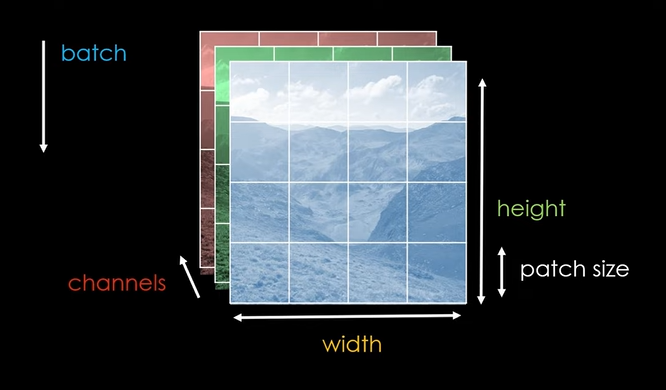
\includegraphics[width=4in]{img/colorbatch.png}
    \caption{\textit{Image with RGB color channels}}
\end{figure}\\
The images undergo resizing and conversion into tensors, representing the initial phase of the process. Following this, the "PatchEmbedding" module is employed to reshape the tensors. This reshaping step plays a pivotal role, setting the stage for a bilinear transformation that ultimately yields embedding vectors. A bilinear transformation was utilized on flattened image patches of one-dimensional sequence, to map them to a desired dimension.\\

Einops-Einstein Operation, is a Python library that was used which simplifies tensor operations. Inspired by Einstein summation conventions, it offers an expressive syntax for reshaping and reducing and manipulation of tensors. \\

After completing the patching process, the original positions of the patches within an image becomes unknown. To address this, position embedding is employed. Since the attention mechanism in transformers is position-independent, position embedding is introduced to enable the model to comprehend the specific locations of each patch in the original image. A vector is assigned to each patch, representing its unique position within the image. The values within these position embedding vectors are derived from sine and cosine functions.\\

The positional encoding can be obtained as:\\
\\
\[
    PE_{(pos, 2i)} = \sin\left(\frac{pos}{{10000}^{(2i/d)}}\right)
\]

\[
    PE_{(pos, 2i+1)} = \cos\left(\frac{pos}{{10000}^{(2i/d)}}\right)
\]
\\
Where:
\begin{align*}
    \text{pos} & : \text{the position of the token in the sequence.} \\
    i          & : \text{the dimension of the positional encoding.}  \\
    d          & : \text{the dimension of the model or embedding.}
\end{align*}

\begin{figure}[htbp]
    \centering
    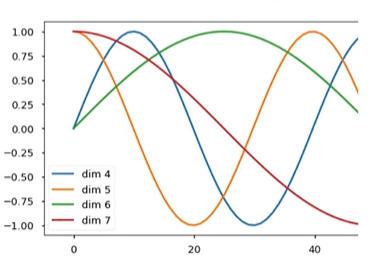
\includegraphics[width=4in]{img/plot for sine and cosine wave.png}
    \caption{\textit{Value vs Position graph for sine and cosine wave}}
\end{figure}

\begin{figure}[htbp]
    \centering
    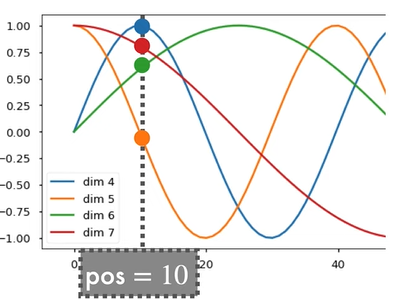
\includegraphics[width=4in]{img/pos 10.png}
    \caption{\textit{Graph for sine and cosine wave  at position 10}}
\end{figure}
For a patch at position 10, the values in its associated position embedding vectors is equivalent to to corresponding values intersecting within the curve as shown in the graph.\\

In the process of adding position embeddings to an image, we introduced a special vector known as the CLS token, where CLS stands for Classification Token. The CLS token is a unique vector assigned to each input image. Initially, it receives random values and is considered a placeholder. However, as the model learns, these values are adjusted based on the information gathered from all other input patches. This adjustment process makes the CLS token a "learnable vector," as it evolves during training to contribute valuable information for the classification task.

\begin{figure}[htbp]
    \centering
    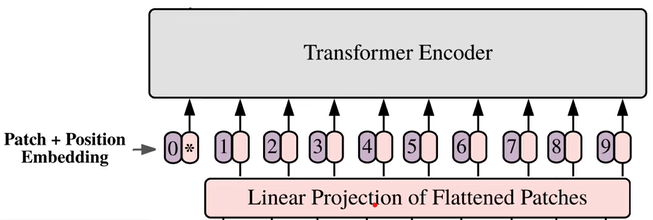
\includegraphics[width=5in]{img/CLS token.png}
    \caption{\textit{CLS Token and position embedding vectors}}
\end{figure}

The CLS token functions as a universal feature extractor, capturing the essence of the entire image. This extracted information can then be utilized for various tasks downstream. The learning positional embeddings helps reduce inductive biases. These embeddings are added on top of input embedding vectors and are not concatenated with them.\\
\\
The Embedded Patches are then passed onto the Encoder section of the model.\\
\begin{figure}[htbp]
    \centering
    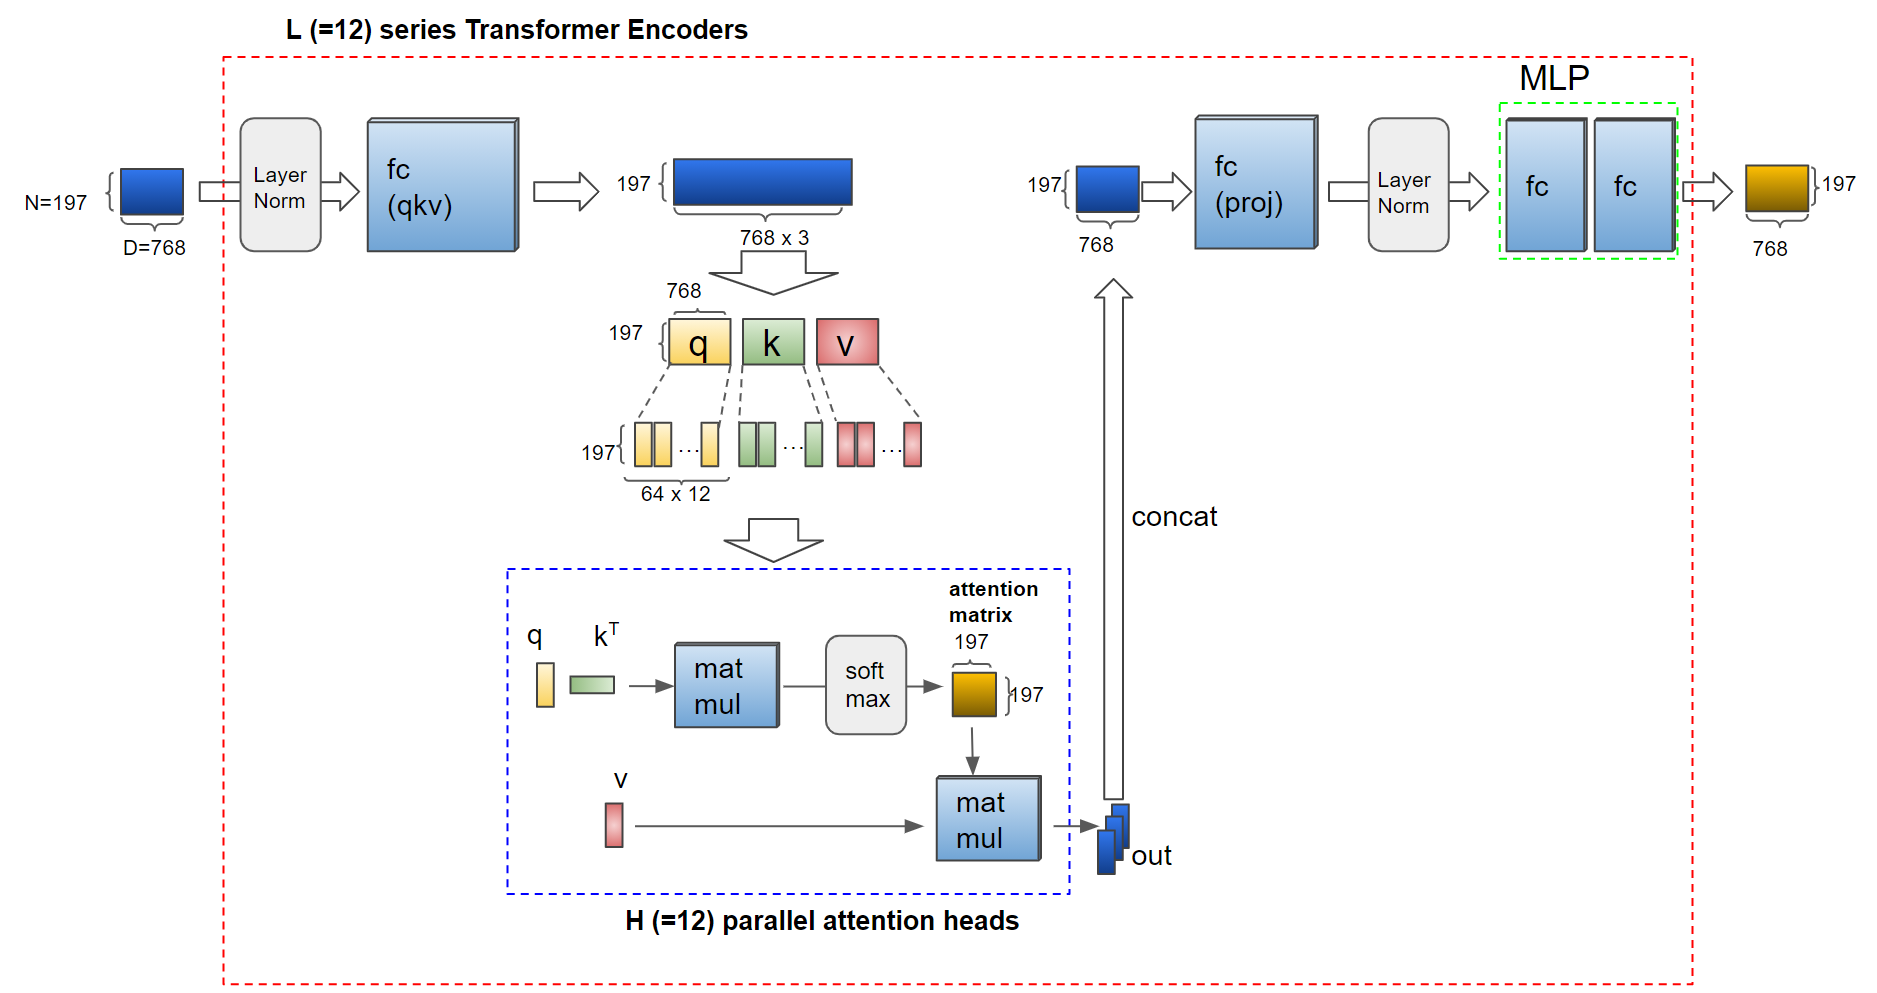
\includegraphics[width=6.3in]{img/transformer_encoder.png}
    \caption{\textit{Transformer Encoder}}
\end{figure}\\

Multihead attention is a mechanism designed to capture different aspects or relationships within input sequences. It involves splitting the input into multiple heads or sets, each with its own set of learned weights. The attention mechanism is then applied independently to each head in parallel.
The multihead attention is the scaled dot product attention mechanism of the transformer and allows to share info between different inputs.\\

In multihead attention, there are three primary inputs:\\

\textbf{Query (Q):} This represents the set of queries used to retrieve information from the input sequence. It is usually derived from the input data and is transformed to capture relevant features.\\

\textbf{Key (K):} The key input consists of keys associated with each element in the input sequence. Like the query, it is derived from the input data and aims to provide information about the relationships between different elements.\\

\textbf{Value (V):} The value input includes the values or content associated with each element in the input sequence. It also comes from the input data and provides the actual information that will be weighted and combined based on the attention mechanism.\\

The Multihead attention process is also regarded as the process where there is inter linkage between the inputs such that exchange of information takes place. To put these Q, K and V to a simple understanding, value is the component that actually is communicated in multihead attention process, query is equivalent for "what i am looking for" and key is equivalent for "what i have."\\

For further explanation  on Multihead Attention, suppose we have inputs to attention blocks of N embeddings (total N+1 including CLS token) and dimension D. With the help of N and D, a stacked matrix can be obtained.
\[ X \in \mathbb{R}^{N \times D}\]

For a single head attention we project each patch embeddings for 3 separate iteration to produce the key, queries and values. The three matrices to produce the keys, queries and values would be:
\[ W^Q \in \mathbb{R}^{D\times d_k}\]
\[ W^K \in \mathbb{R}^{D \times d_k}\]
\[ W^V \in \mathbb{R}^{D \times d_v}\]
Where:
\begin{align*}
    d_k & : \text{the dimension of query and key .} \\
    d_v & : \text{the dimension of values.}
\end{align*}
Therefore, the key(K), query(Q) and value(V) can be obtained when the original embedding matrix X is multiplied with the above mentioned matrices.
\[Q = X.W^Q \in \mathbb{R}^{N\times d_k}\]
\[K = X.W^K \in \mathbb{R}^{N\times d_k}\]
\[V = X.W^V \in \mathbb{R}^{N\times d_v}\] \\

The multihead attention will contain 'h' numbers of heads, each head representing as a single. All these multiple heads undergo computation in parallel. \\

The general form of  scaled dot-product attention is given as:
\[\text{Attention}(h) = \text{softmax}\left(\frac{Q_h * K_h ^T}{\sqrt{d_k}}\right) V_h\]
The softmax is applied along the rows of the matrix to normalize them to probability vectors and $d_k$ helps in avoiding peaky affinities.When attention distributions are too peaky, it suggests the model is assigning a significantly higher weight to a small subset of elements in the input sequence while largely ignoring the rest.\\

Finally, \[\text{Multihead Attention} = \text{concat} (h_1, h_2, h_3,...,H)* W^o \]

$W^0$ is added to ensure the right dimension is obtained.


\begin{figure}[htbp]
    \centering
    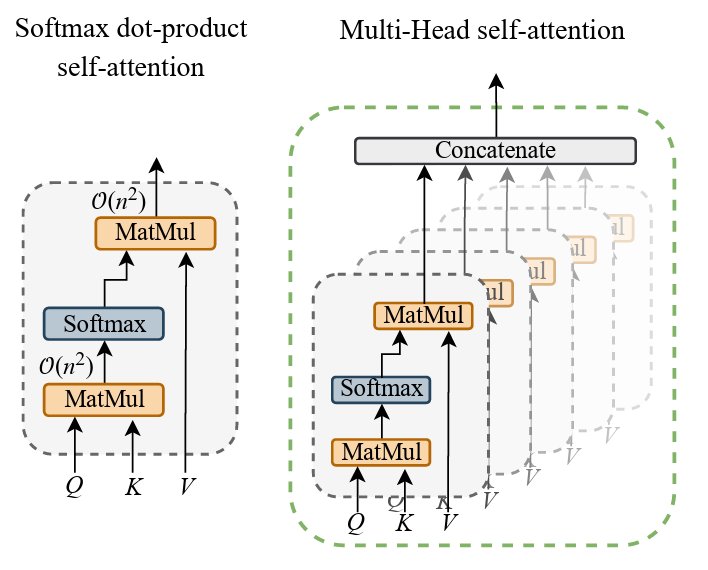
\includegraphics[width=5in]{img/Attentionfig.png}
    \caption{\textit{Attention head visualization}}
\end{figure}

The asymptotic complexity, often denoted as Big O notation, for Multi-Head Attention (MHA) in the Transformer model is typically expressed as\[ O(N \cdot d^2 \cdot H)\], where:
\begin{itemize}
    \item $N$ is the sequence length,
    \item $d$ is the dimensionality of the model's hidden representations,
    \item $H$ is the number of attention heads.
\end{itemize}
Because of this when processing long sequences, the computational cost of Multihead Attention, can be substantial.\\

At present context, multihead attention doesn't require building from scratch; instead, it can be accessed through a pre-existing module.\\

After the MultiHead Attention layer, an essential component is the Multi-Layer Perceptron (MLP). The MLP comprises two bilinear layers, incorporating the GeLU activation function and followed by a Dropout layer. Unlike in Multihead Attention, where components interact with each other, in MLP, the inputs are treated independently and don't communicate with each other directly.\\

The expression for MLP is given as:\\

\[\text{MLP}(x) = W_2 \cdot \sigma(W_1 \cdot x + b_1) + b_2\]
where:
\begin{align*}
    x      & : \text{the input vector,}                                \\
    W_1    & : \text{the weight matrix for the first bilinear layer,}  \\
    b_1    & : \text{the bias vector for the first layer,}             \\
    \sigma & : \text{GeLU activation function (non-linear),}           \\
    W_2    & : \text{the weight matrix for the second bilinear layer,} \\
    b_2    & : \text{the bias vector for the second layer.}
\end{align*}
Usually, an expansion factor of 4 is commonly employed as it is observed to be effective based on empirical evidence.\\
\\

\begin{figure}[htbp]
    \centering
    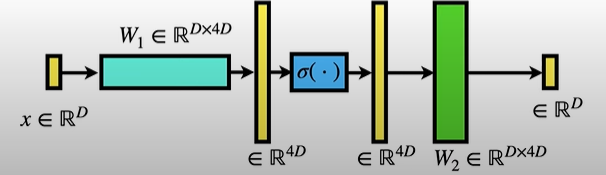
\includegraphics[width=5in]{img/MLP workings.png}
    \caption{\textit{Workings in MLP}}
\end{figure}
\newpage
\begin{figure}[htbp]
    \centering
    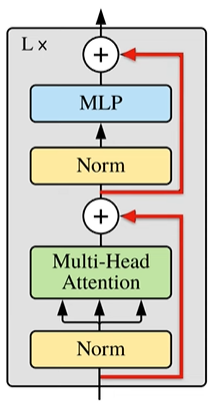
\includegraphics[width=2in]{img/residual connection.png}
    \caption{\textit{Residual connection}}
\end{figure}
The Residual connection, also known as Skip connection, addresses the vanishing gradient issue by facilitating smoother gradient flow throughout the network during back-propagation. By incorporating a shortcut that maintains an identity mapping, residual connections empower the model to learn residual features, capturing the distinctions between the input and the output of the layer. In this procedure, the respective inputs are applied back into the result from obtained form MLP and MHA.\\

The general form can be represented as:\\

For Multihead Output\\
\[(Y) = (X)+\text{MHA (Normalization (X))}\]

For MLP Output
\[(OUTPUT) = (Y)+\text{MLP (Normalization (Y))}\]
where:
\begin{align*}
    \text{X} & : \text{Input for MHA}                 \\
    \text{Y} & : \text{Output from MHA Input for MLA} \\
\end{align*}

Lastly, Layer Normalization, provided by Keras through the LayerNormalization module, is used for the normalization. Its integration helps stabilize training and maintain proper feature scaling, contributing to improved performance in image recognition tasks. It provides multiple benefits, such as enhanced training stability, reduction of internal covariate shifts, and improved generalization. By ensuring uniform activation distributions across various layers, it facilitates smoother optimization, leading to an overall more robust and efficient model.
\subsection{Model Data Flow}

\begin{figure}[htbp]
    \centering
    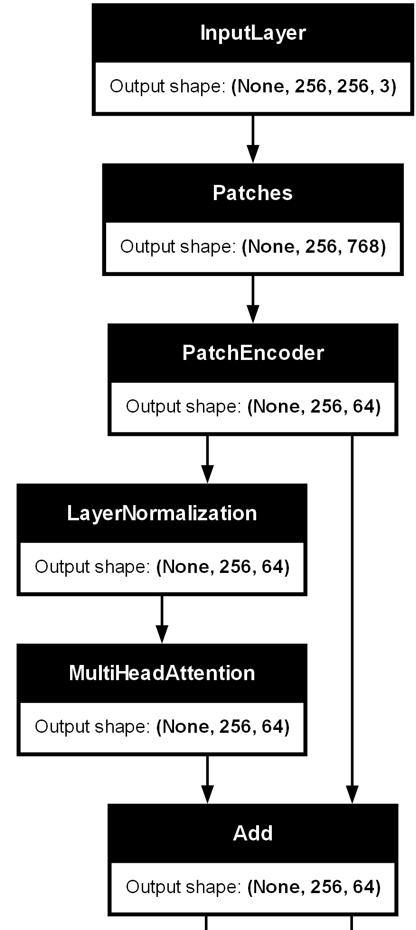
\includegraphics[width=3in]{img/1STPHASE.png}
    \caption{\textit{Data Flow in the First Phase of Model Building}}
\end{figure}

\begin{figure}[htbp]
    \centering
    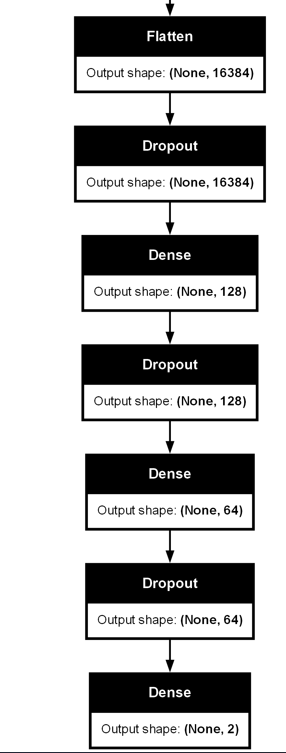
\includegraphics[width=3in]{img/2NDPHASE.png}
    \caption{\textit{Data Flow in the Second Phase of Model Building}}
\end{figure}
 

\newpage
\subsection{Application Development }

\subsubsection{Frontend Mobile App Development}


\begin{itemize}
      \item\textbf{Overview}:\\
      Our frontend is designed to provide a user-friendly interface for interacting with the Deepfake Detection App using React Native. It includes features such as user authentication, profile management, and image testing for deepfake detection.

      \item\textbf{Components}:\\
      The frontend consists of several components:

      \begin{itemize}
            \item \textbf{Login Screen}: The login screen serves as the entry point for users to access the application. It presents a clean and intuitive interface where users can input their credentials to authenticate and gain access to their account.

            \item \textbf{Signup Screen}: The signup screen facilitates the registration process through a form where users can input their personal details such as name, email address, and desired password. Upon successful completion of the signup process, users are usually redirected to the login screen to authenticate and access their newly created account.

            \item \textbf{Media Testing Screen}: The media testing screen provides functionality for users to analyze both images and videos for the presence of deepfakes or other forms of manipulation. It offers a straightforward interface for users to upload media files from their device or capture new ones using the device's camera. After uploading a file, the screen initiates a deepfake detection process, using trained modeled to analyze the media and determine its authenticity. The result of the analysis is then displayed to the user, indicating whether the media is likely to be genuine or altered.

            \item \textbf{Profile Screen}: The profile screen provides users with a personalized view of their account information.

            \item \textbf{History Screen}: The history screen allows users to view a chronological record of their past activities within the application. This include a history of logged-in sessions, image testing results. Each entry in the history list includes details such as the date and time of the activity, along with results.
      \end{itemize}

            \item \textbf{Styling}:\\
            The frontend of our application is styled to ensure a seamless user experience, blending custom-styled components with predefined elements from React Native. Custom-styled components are utilized to maintain a cohesive visual identity and streamline the design process, promoting consistency and efficiency.

            \item\textbf{Navigation}:\\
            We have implemented navigation between screens using the React Navigation library. This allows users to navigate seamlessly between different sections of the app.
\end{itemize}

\subsubsection{Backend API Development}

We have used FastAPI to build backend API, providing robust and efficient routing for handling requests and deploying machine learning models trained with Keras for deepfake detection.

\begin{itemize}
      \item \textbf{Overview}:\\
            The backend API serves as the foundation for our Deepfake Detection App, handling various endpoints for user authentication, media testing, and model deployment. It integrates seamlessly with the frontend to provide a cohesive user experience.

      \item \textbf{Endpoints}:\\
            The backend API consists of the following endpoints:

            \begin{itemize}

                  \item \textbf{Authentication Endpoint}\\
                        The authentication endpoint provides a secure mechanism for users to log in and access their accounts. Upon receiving login credentials, the endpoint verifies the provided username and password by comparing them with the hashed credentials stored in the database. To enhance security, the passwords are hashed using the bcrypt hashing algorithm before being stored in the database. If the credentials match, the endpoint generates a JSON Web Token (JWT) containing user information and a unique identifier, which is signed using a secret key. This token is then returned to the client and can be used for subsequent authorized access to protected resources without the need to repeatedly provide credentials.

                        \begin{figure}[htbp]
                              \centering
                              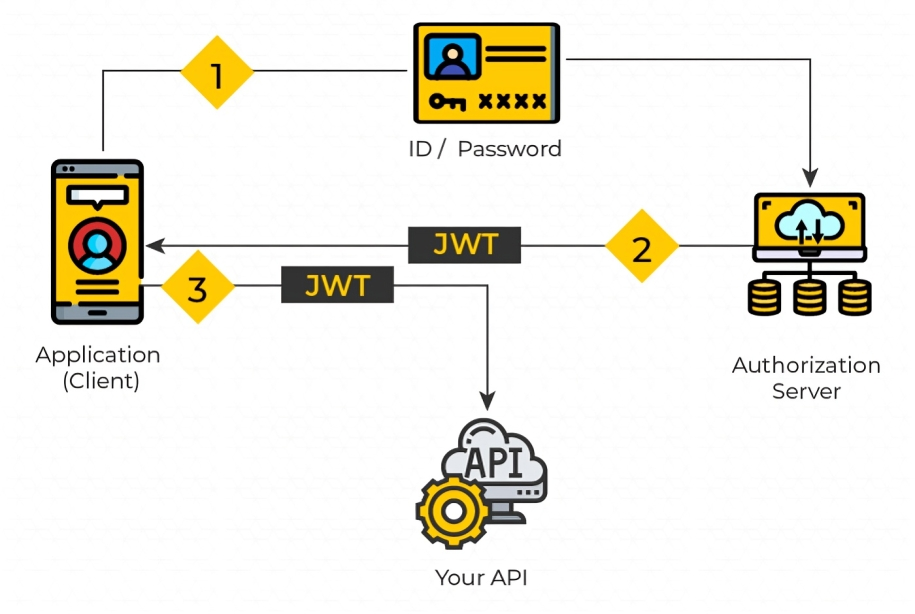
\includegraphics[width=5in]{img/JSON-Web-Tokens-01.png}
                              \caption{JWT Workflow}
                        \end{figure}

                  \item \textbf{Signup Endpoint}:\\
                        The signup endpoint facilitates user registration by processing signup requests and creating new user accounts in the database. The password is securely hashed using the bcrypt algorithm before being stored in the database to protect user privacy. After successful validation and hashing, the endpoint creates a new user account with the provided details and assigns a unique identifier.

                        \begin{figure}[htbp]
                              \centering
                              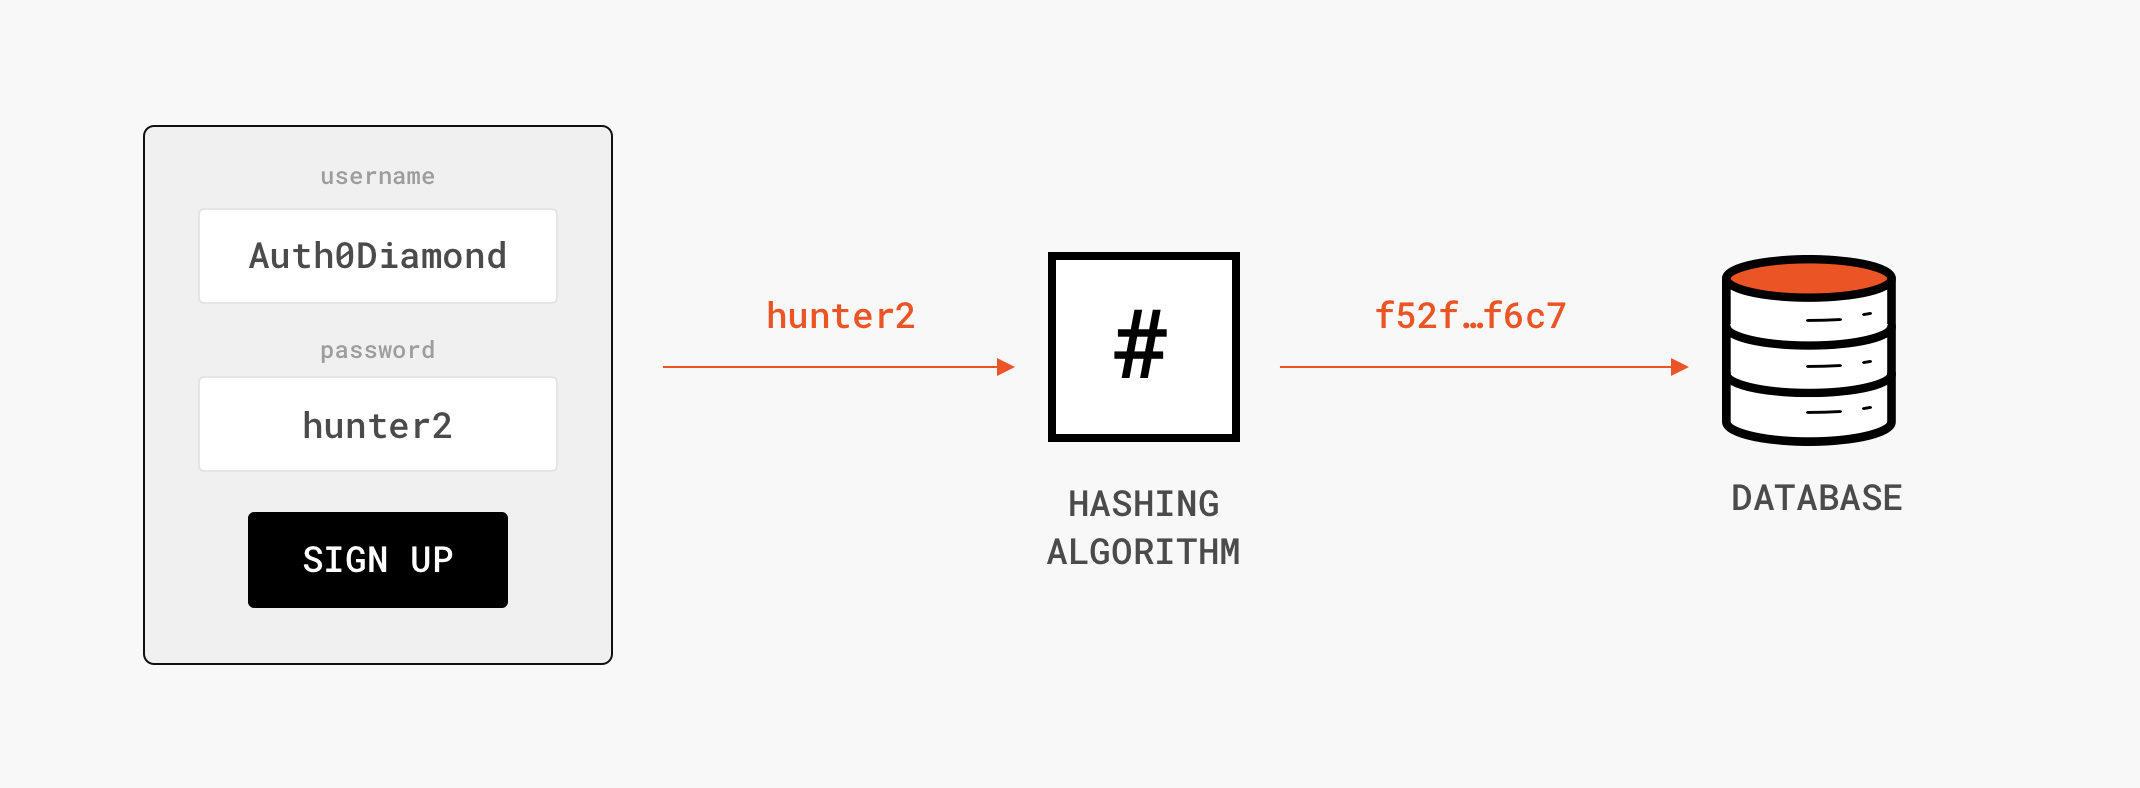
\includegraphics[width=5in]{img/example-of-hashing-during-signup.png}
                              \caption{Hashing}
                        \end{figure}
                  \item \textbf{Media Testing Endpoint}:\\
                        This endpoint is responsible for analyzing images and videos uploaded by users to detect the presence of deepfakes. It utilizes machine learning models deployed with Keras to perform deepfake detection and returns the analysis results to the frontend for display.

                  \item \textbf{Profile Endpoint}:\\
                        The profile endpoint handles requests related to user profiles, allowing users to view their account information.

                  \item \textbf{History Endpoint}: The history endpoint manages user activity logs, maintaining a record of past interactions within the application. It stores information such as login sessions, media testing results, and other relevant data for reference and analysis.
            \end{itemize}

      \item \textbf{Routing and Middleware}:\\
            FastAPI's routing system facilitates the organization and management of various endpoints within our backend application. Through intuitive decorators and path operations, we define the routes that handle incoming HTTP requests and specify the corresponding logic to execute for each request type (GET, POST, PUT, DELETE, etc.).

            Additionally, middleware functions play a crucial role in enhancing the capabilities and security of our backend infrastructure. These middleware components intercept incoming requests and responses, allowing us to implement cross-cutting concerns such as authentication, logging, request validation, and error handling.

            \begin{figure}[htbp]
                  \centering
                  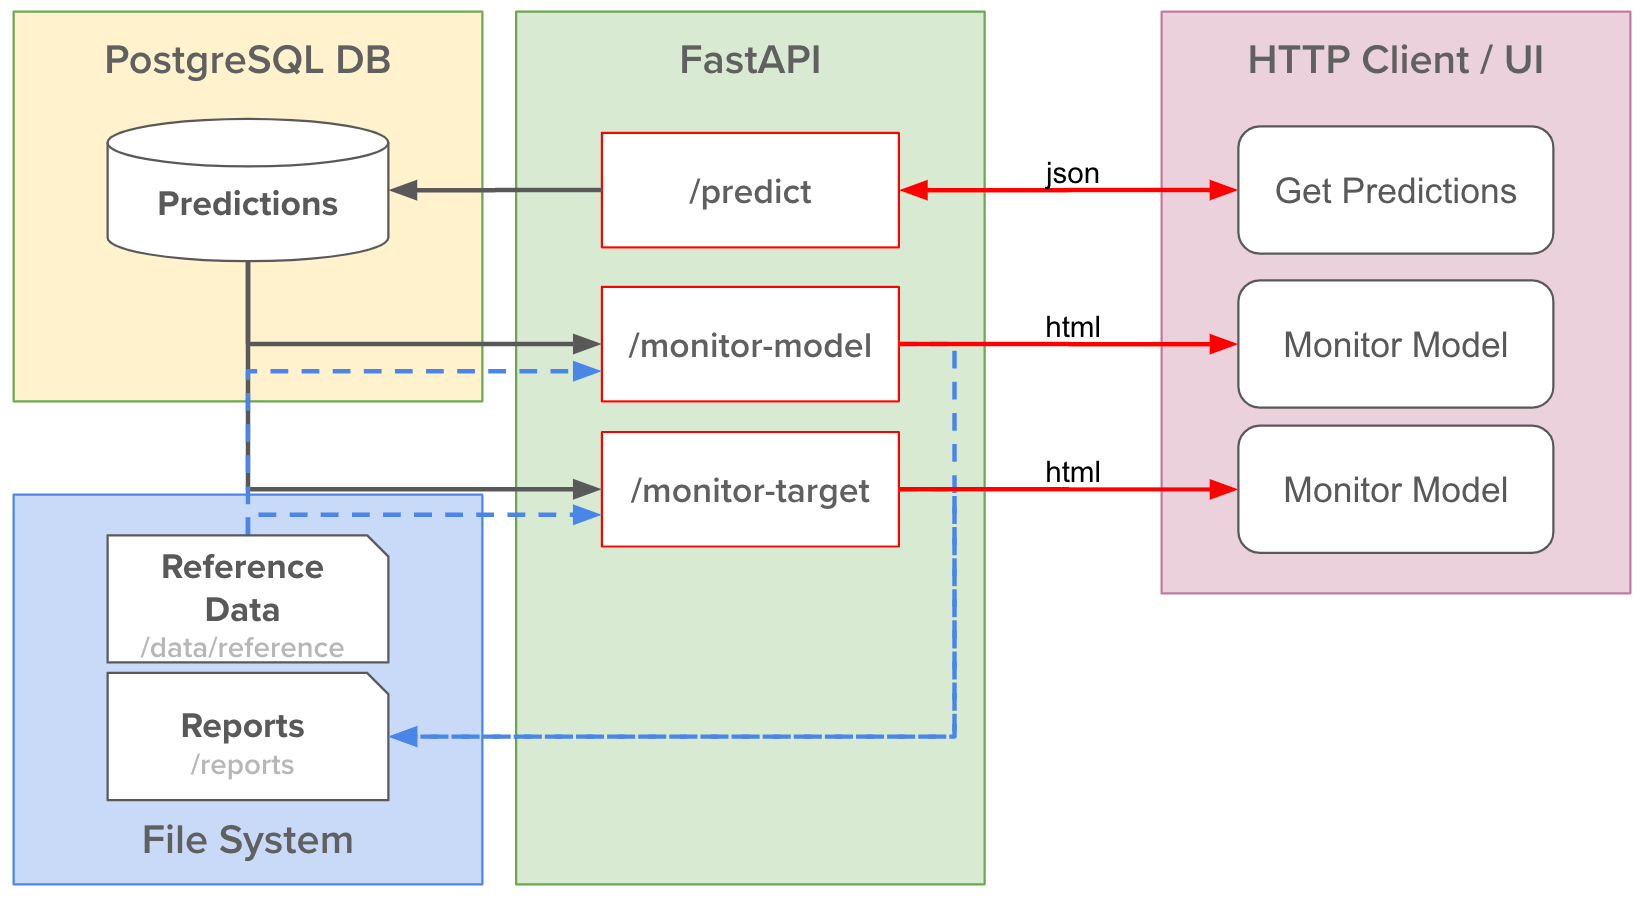
\includegraphics[width=6in]{img/image_2024-02-23_19-12-39.png}
                  \caption{System Workflow Architecture}
            \end{figure}

      \item \textbf{Model Deployment}:\\
            Our backend API integrates machine learning models trained with Keras for deepfake detection. These models are deployed as endpoints within the API, allowing them to process incoming media files and generate predictions on-the-fly. Model deployment is handled efficiently to ensure optimal performance and scalability.

\end{itemize}


\newpage




\newpage



\section{Result and Analysis}
\subsection{Parameters}
\begin{table}[h]
    \centering
    \renewcommand{\arraystretch}{1.5} %
    \begin{tabular}{|c|c|}
        \hline
        \textbf{Parameters}                     & \textbf{Value}      \\
        \hline
        \textbf{Total Datasets}                 & 6                   \\
        \hline
        \textbf{Total images}                   & 446K                \\
        \hline
        \textbf{Trained images (real and fake)} & 203K , 203K         \\
        \hline
        \textbf{Tested images (real and fake)}  & 10K , 10K           \\
        \hline
        \textbf{Validation (real and fake)}     & 10K , 10K           \\
        \hline
        \textbf{Balanced}                       & True                \\
        \hline
        \textbf{Epochs}                         & 10                  \\
        \hline
        \textbf{Batch Size}                     & 32                  \\
        \hline
        \textbf{Image Size}                     & 256 x 256           \\
        \hline
        \textbf{Channels}                       & 3                   \\
        \hline
        \textbf{Patches}                        & 16 x 16             \\
        \hline
        \textbf{Encoder Hidden Layers}          & 12                  \\
        \hline
        \textbf{Encoder Layers Dimension}       & 768                 \\
        \hline
        \textbf{MLP size}                       & 3072                \\
        \hline
        \textbf{ Number of Attention Heads }    & 12                  \\
        \hline
        \textbf{Loss Function}                  & Cross-Entropy Loss  \\
        \hline
        \textbf{Normalization}                  & Layer Normalization \\
        \hline
        \textbf{Activation Function}            & GeLU                \\
        \hline
        \textbf{Dropout Rate }                  & 0.2                 \\
        \hline
        \textbf{Pooling Strategy }              & CLS Token           \\
        \hline
    \end{tabular}
    \caption{Model Parameters}
    \label{tab:model-parameters}
\end{table}
\newpage
\subsection{Evaluation}
\subsubsection{Loss Curve}
\begin{figure}[ht]
    \centering
    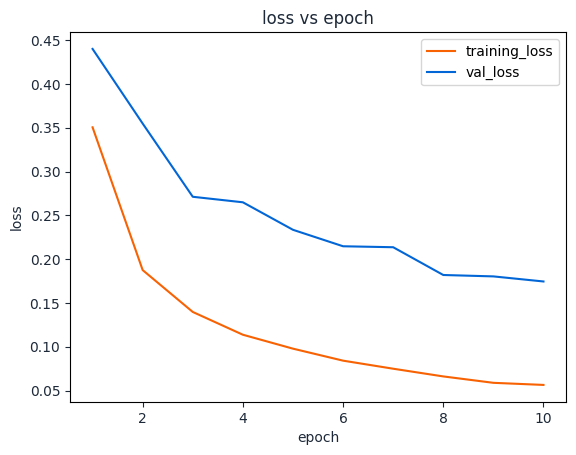
\includegraphics[width= 5in, height =5in ]{img/lossVsAccuracy.png}
    \caption{\textit{Training Vs Validation loss Curve}}
\end{figure}

\newpage
\subsubsection{Accuracy Curve}
\begin{figure}[ht]
    \centering
    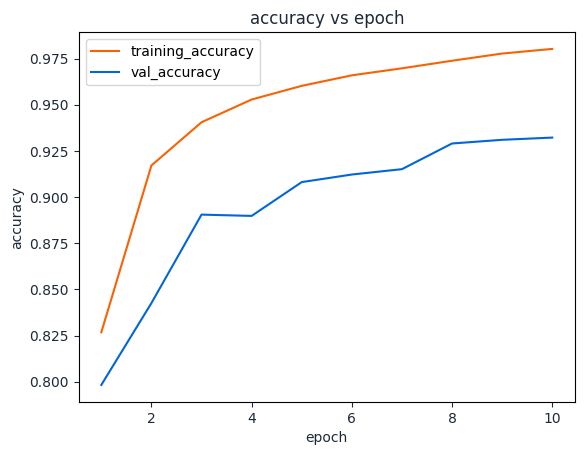
\includegraphics[width=5in, height =5in ]{img/accuracyVsepoch.png}
    \caption{\textit{Training Vs Validation Accuracy Curve }}
\end{figure}
\newpage
\subsubsection{Confusion Matrix}
\begin{figure}[ht]
    \centering
    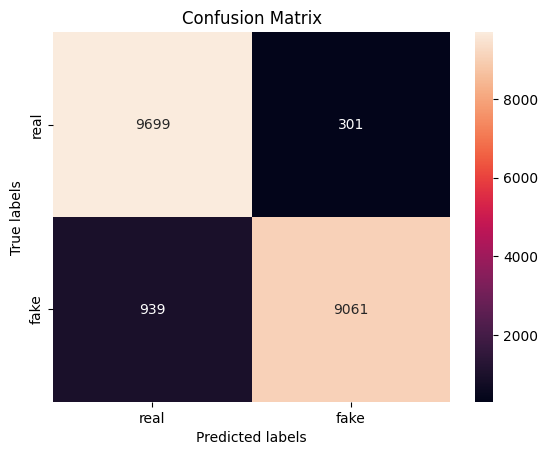
\includegraphics[width=5in, height =5in ]{img/confusionMatrixImage.png}
    \caption{\textit{Confusion Matrix }}
\end{figure}
\newpage
\subsubsection{performance Metrices}

The performance of our model is associated with various metrics such as:
\begin{enumerate}
    \item \textbf{Accuracy:}
          The accuracy metric measures how correctly the model predicts instances by calculating the ratio of correctly classified instances to the total samples.
          \[ Accuracy = \frac{TP + TN}{TP + FP + TN + FN} \]

    \item \textbf{Precision:}
          Precision assesses the model's ability to identify positive samples among the actual positives, calculated as the ratio of true positives to the sum of true positives and false positives.

          \[ Precision = \frac{TP}{TP + FP} \]

    \item \textbf{Recall (Sensitivity or True Positive Rate):}
          Recall measures the model's ability to precisely identify positive samples from the actual positives, calculated as the ratio of true positives to the sum of true positives and false negatives.

          \[ Recall = \frac{TP}{TP + FN} \]


    \item \textbf{F1 Score:}

          The F1 score, a balance between precision and recall, is advantageous in scenarios with unequal class distribution or equal emphasis on both types of errors. It ranges between 0 and 1, with peak performance at 1.

          \[ F1 = \frac{2 \cdot Precision \cdot Recall}{Precision + Recall} \]

\end{enumerate}
\newpage
\subsection{Model Inference Results }
\begin{enumerate}
    \item \textbf{True Positive:}
          \begin{figure}[ht]
              \centering
              
\includegraphics[width= 5in, height =5in ]{img/ranveer.jpg}
              \caption{\textit{True Positive Case}}
          \end{figure}
          \begin{figure}[ht]
              \centering
              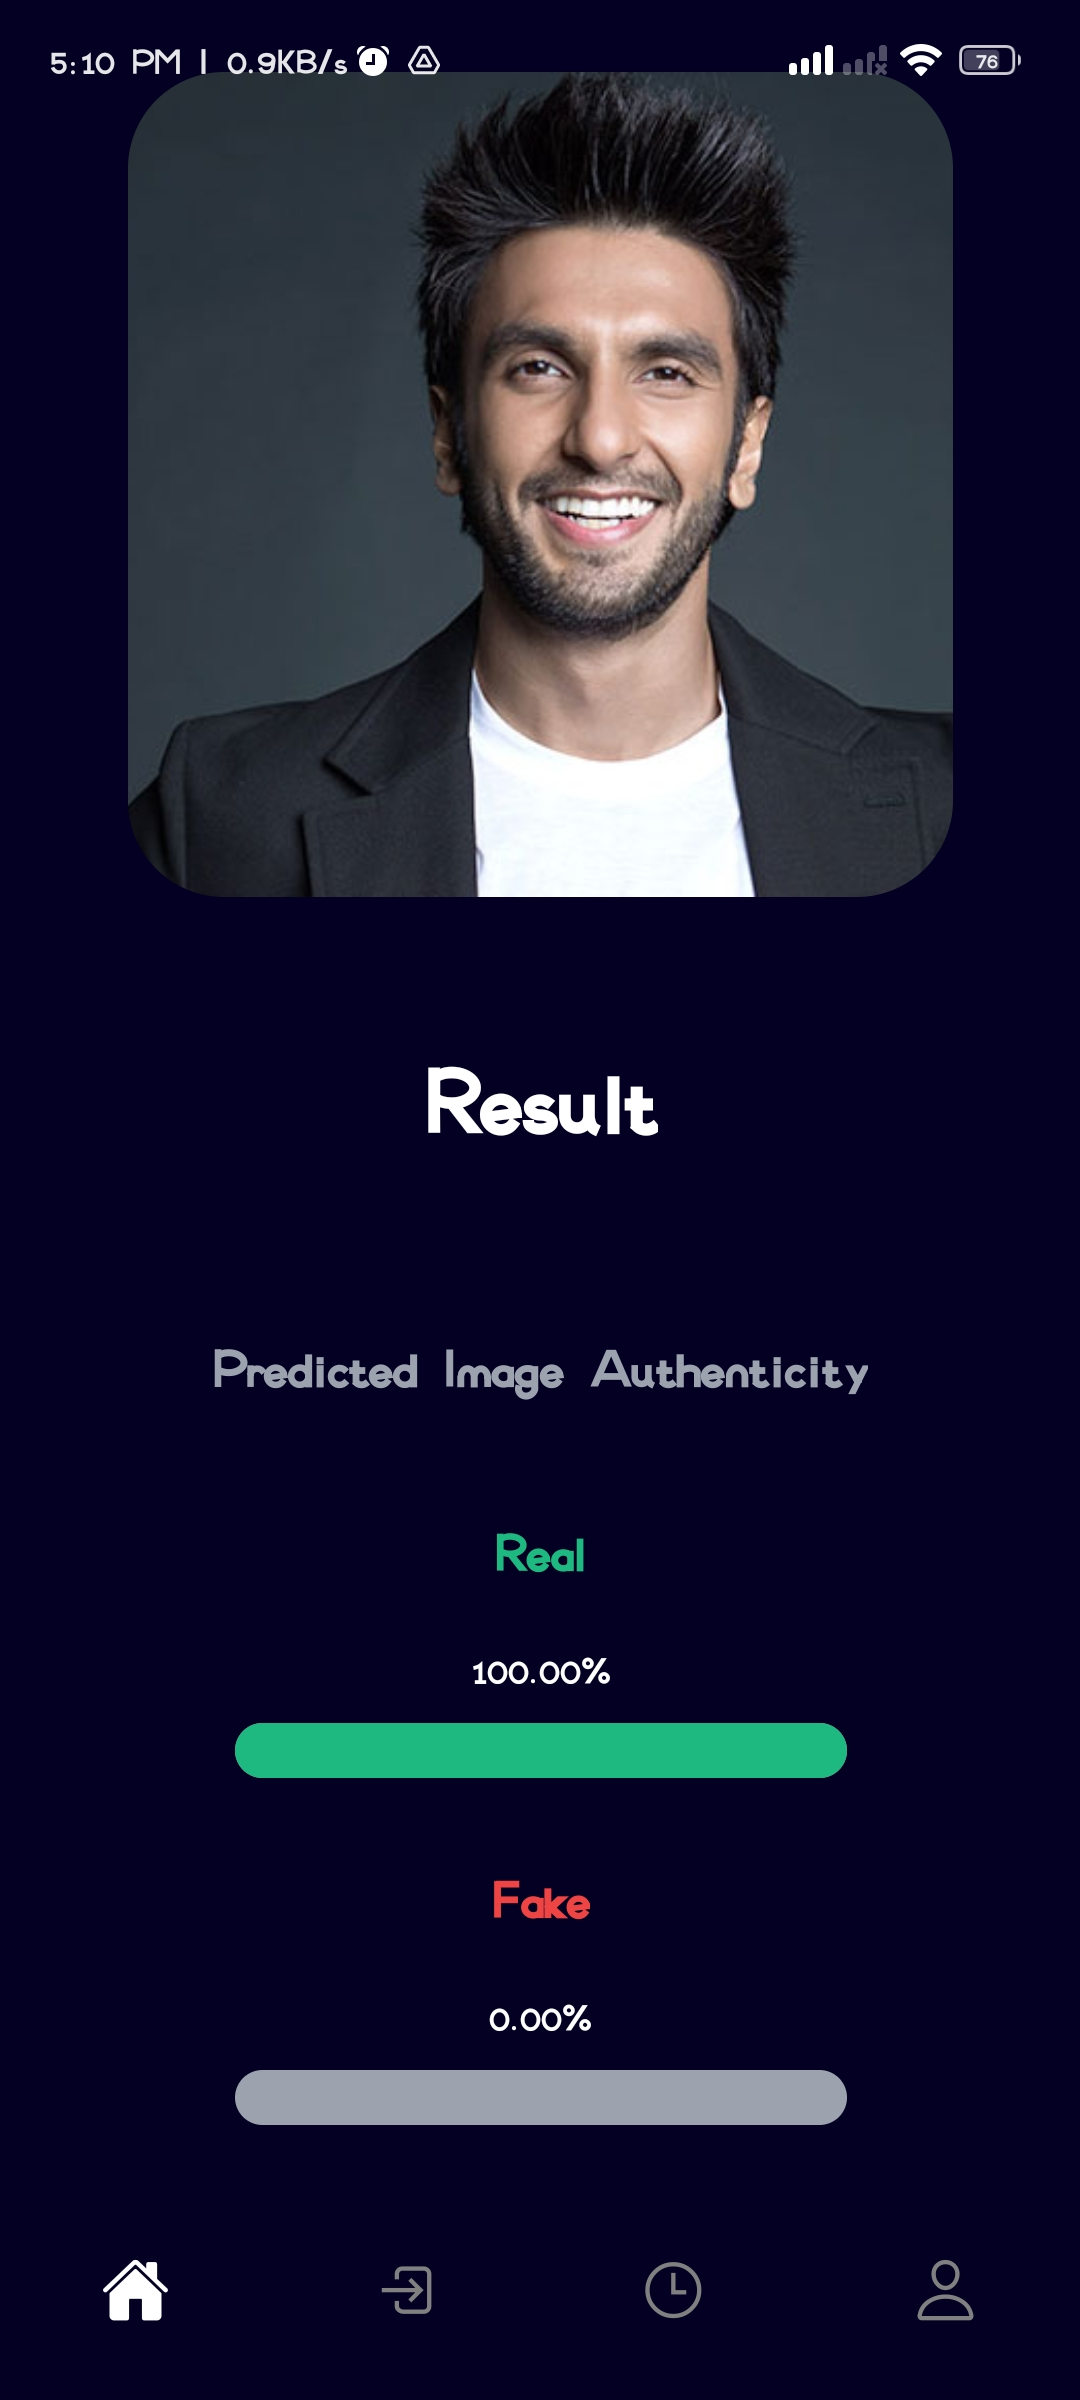
\includegraphics[height =5in  ]{img/ranveerResult.jpg}
              \caption{\textit{Training Vs Validation loss Curve}}
          \end{figure}

          \newpage
    \item \textbf{False Positive:}
          \begin{figure}[ht]
              \centering
              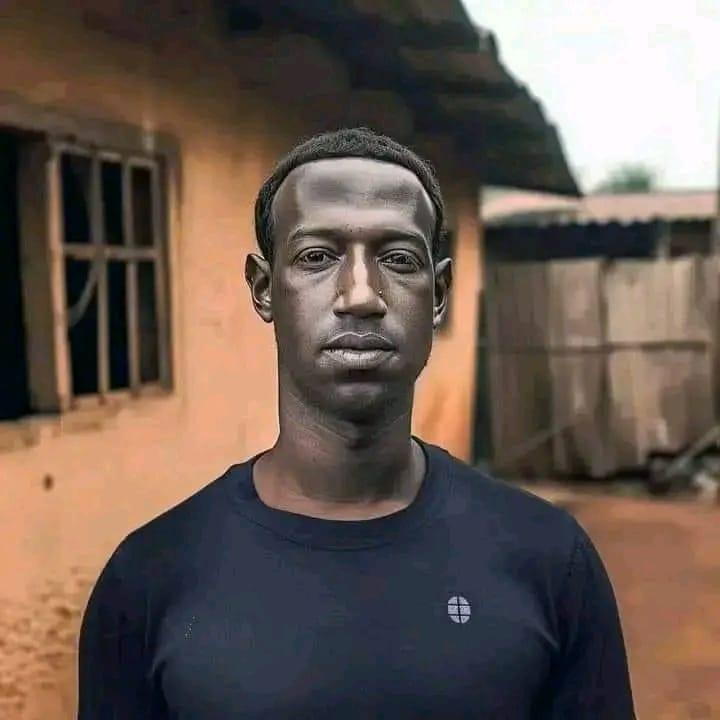
\includegraphics[width= 5in, height =5in ]{img/blckZuke.png}
              \caption{\textit{Training Vs Validation loss Curve}}
          \end{figure}
          \begin{figure}[ht]
              \centering
              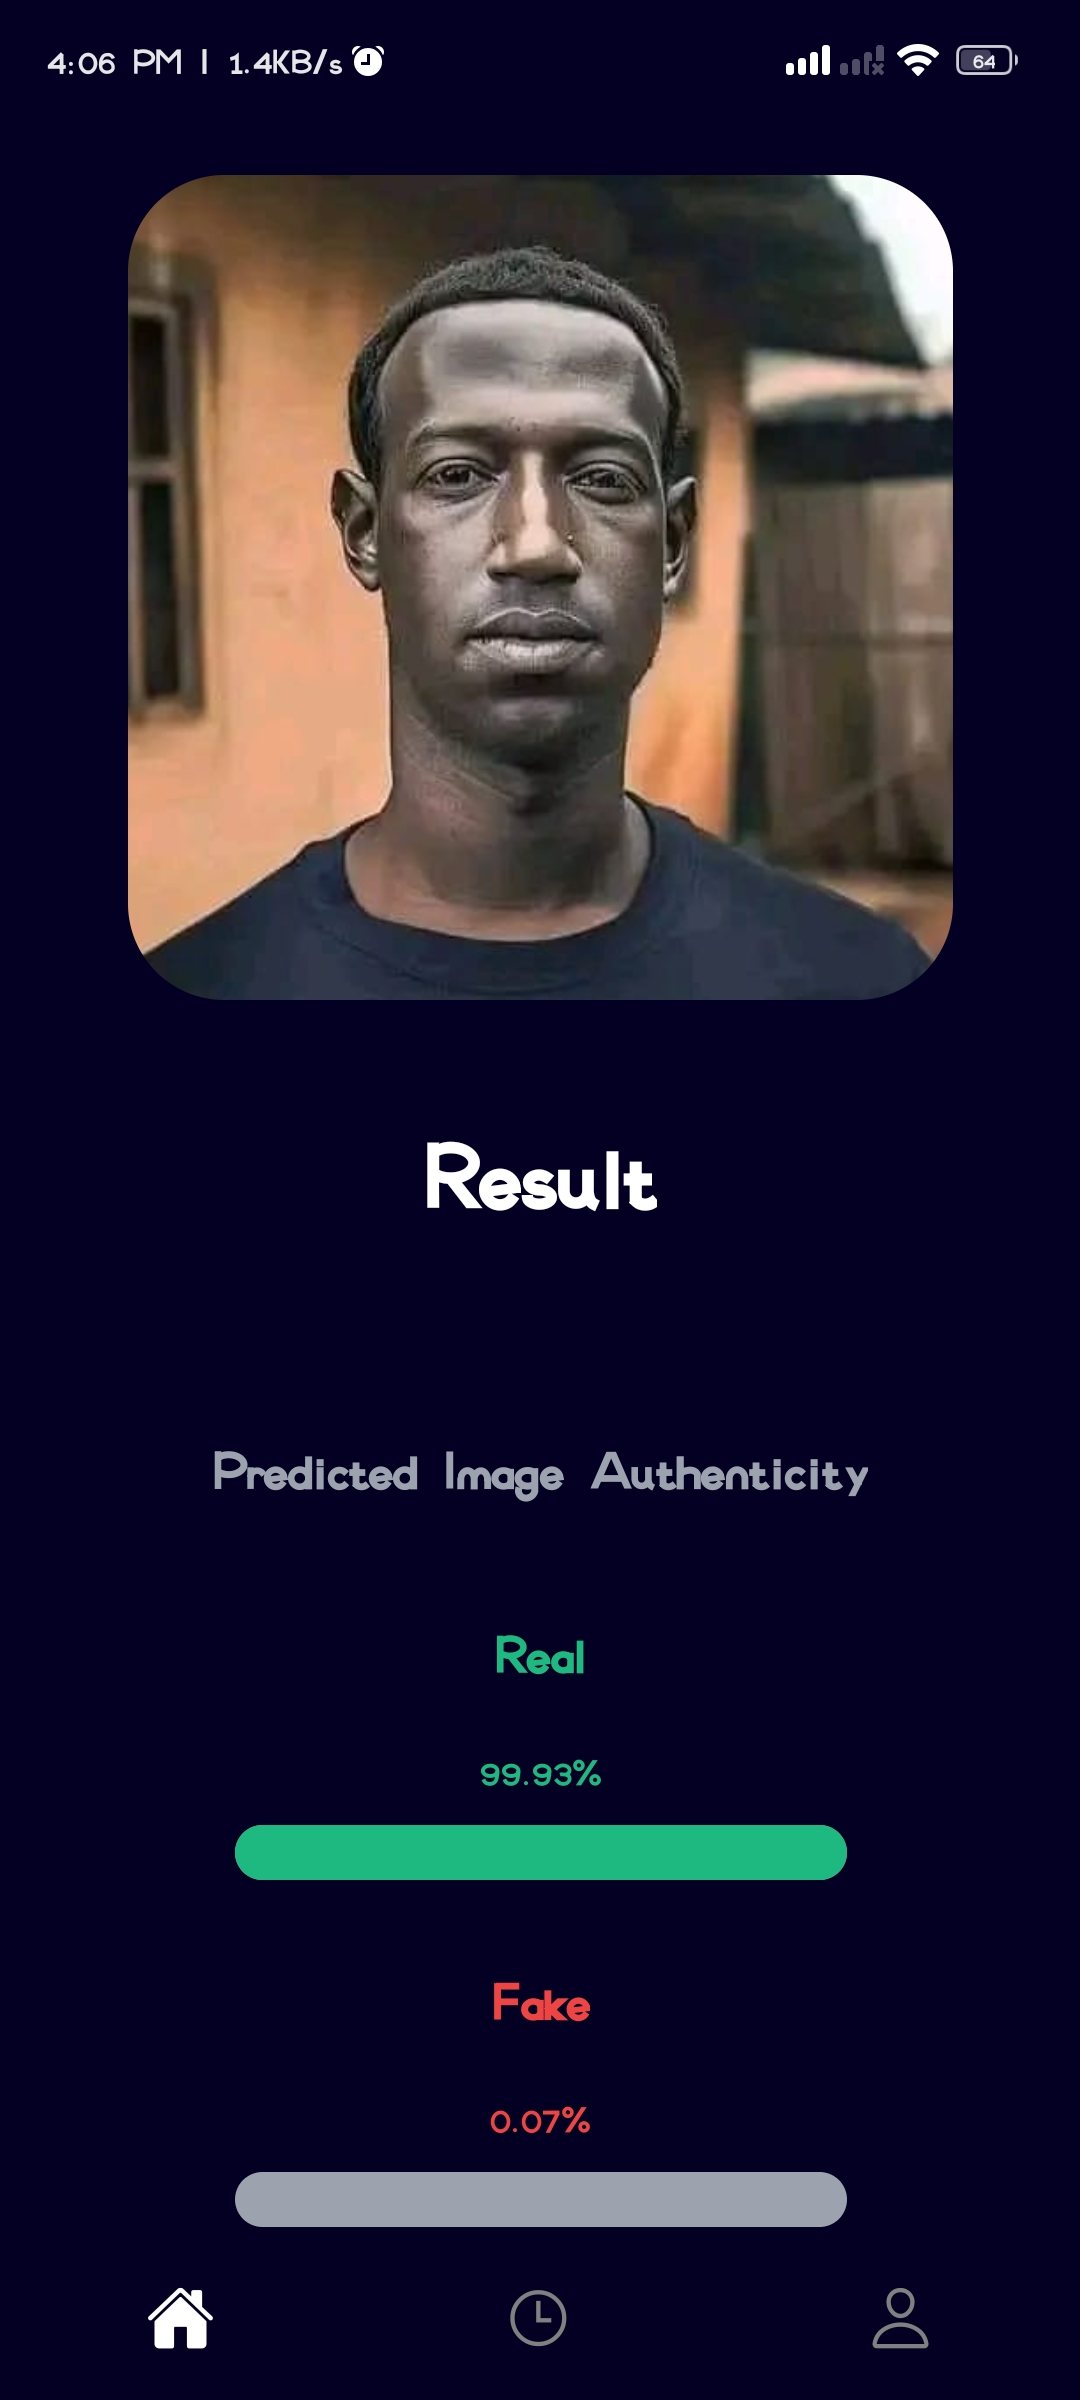
\includegraphics[height =5in  ]{img/blckzukeOutput.jpg}
              \caption{\textit{Training Vs Validation loss Curve}}
          \end{figure}

          \newpage

    \item \textbf{Ture Negative}
          \begin{figure}[ht]
              \centering
              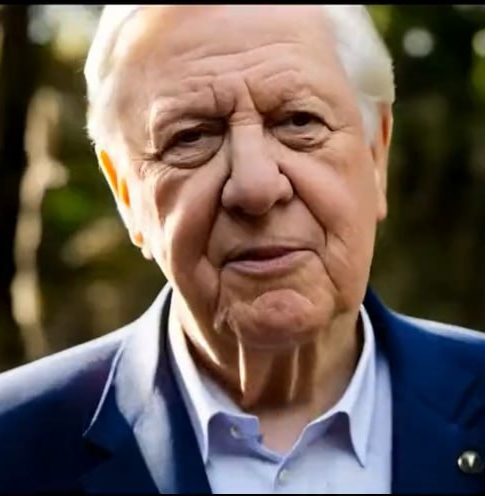
\includegraphics[width= 5in, height =5in ]{img/oldman.jpg}
              \caption{\textit{Training Vs Validation loss Curve}}
          \end{figure}
          \begin{figure}[ht]
              \centering
              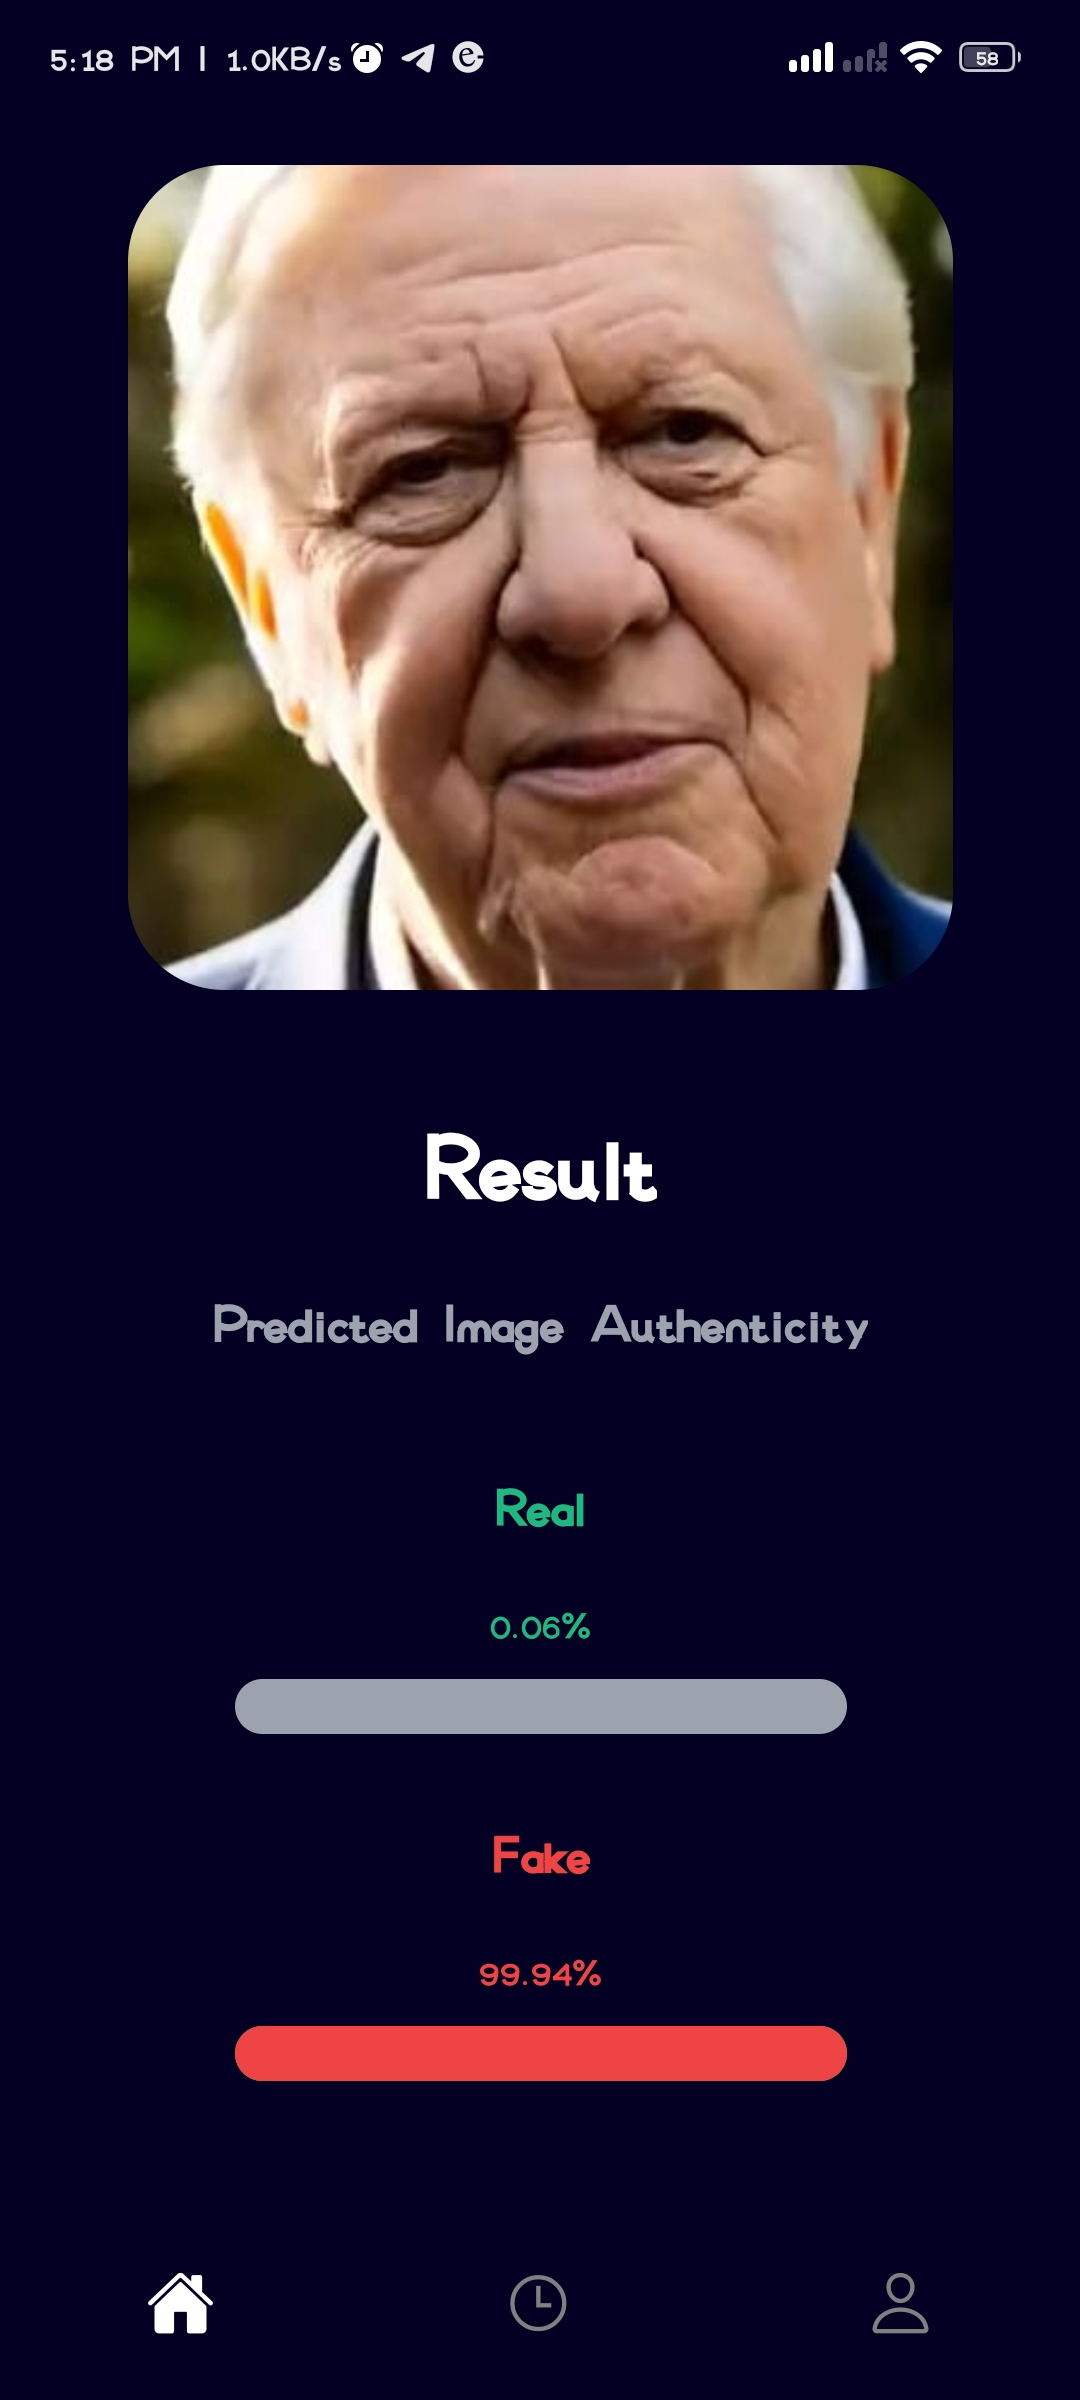
\includegraphics[height =5in ]{img/oldmanResult.jpg}
              \caption{\textit{Training Vs Validation loss Curve}}
          \end{figure}

          \newpage


    \item \textbf{False Negative}
          \begin{figure}[ht]
              \centering
              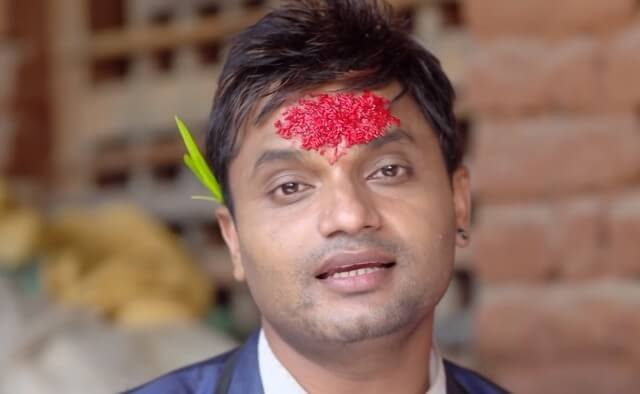
\includegraphics[width= 5in, height =5in ]{img/Nepali-Dashain-Tika-Pictures-Artists.jpg}
              \caption{\textit{Training Vs Validation loss Curve}}
          \end{figure}
          \begin{figure}[ht]
              \centering
              \includegraphics[height =5in ]{img/dashainResult.jpg}
              \caption{\textit{Training Vs Validation loss Curve}}
          \end{figure}


          \newpage

\end{enumerate}
% \subsection{Work Completed}
% \subsubsection{User Interface of Mobile application}
% % \begin{itemize}
% %     \item a
% % \end{itemize}
% \subsubsection{Backend}
% % \begin{itemize}

% % \end{itemize}
% \subsubsection{Machine Learning Model}
% % \begin{itemize}

% % \end{itemize}

% \subsection{Work Remaining}
% % \begin{itemize}

% % \end{itemize}

\newpage
\subsection{UI of Project}
We have used React Native for the development of the mobile application.
Following are the UIs with user authentication, login page and home page where we can upload images to be classified as fake and real.\\

\begin{figure}[ht]
    \centering
    \includegraphics[ height =5in ]{img/loginv3.png}
    \caption{\textit{Login Page }}
\end{figure}

\begin{figure}[ht]
    \centering
    \includegraphics[height= 5in]{img/signup.png}
    \caption{\textit{Sign-up form}}
\end{figure}
\begin{figure}[ht]
    \centering
    \includegraphics[height =5in ]{img/Homepage.png}
    \caption{\textit{Home Page}}
\end{figure}

\begin{figure}[ht]
    \centering
    \includegraphics[height =5in ]{img/uploaderv3.png}
    \caption{\textit{Uploader}}
\end{figure}

\begin{figure}[ht]
    \centering
    \includegraphics[height= 5in]{img/Results.png}
    \caption{\textit{Result}}
\end{figure}

\begin{figure}[ht]
    \centering
    \includegraphics[height= 5in]{img/Historyv2.png}
    \caption{\textit{History page}}
\end{figure}


\begin{figure}[ht]
    \centering
    \includegraphics[height= 5in]{img/profilev2.png}
    \caption{\textit{Profile page}}
\end{figure}
\newpage


% \section{FUTURE ENHANCEMENTS}
% There is always a scope for enhancements in any developed system, especially
% when the project build using latest trending technology and has a good scope in
% future.
% \begin{itemize}
%     \item Web based platform can be upscaled to a browser plugin for ease of access to
%           the user.
%     \item Currently only Face Deep Fakes are being detected by the algorithm, but the
%           algorithm can be enhanced in detecting full body deep fakes.
% \end{itemize}

\newpage


% \section{LIMITATIONS}
% \begin{itemize}
%     \item Deepfake detection projects face challenges due to rapidly evolving techniques and the need for diverse training data.
%     \item Adversarial attacks can exploit weaknesses in detection algorithms, making deepfakes harder to identify accurately.
%     \item Deepfake detection algorithms often require significant computational resources, limiting their applicability on resource-constrained devices.
% \end{itemize}
\newpage

\section{CONCLUSION}
 In summary, our project for spotting fake media using Vision Transformers is a strong and easy-to-use solution. The simple interface makes it easy for users to upload content and see results clearly. Our system is really efficient and effective for detection of manipulated contents, with an impressive average accuracy of about 92.85\% in different tests. It stays strong against real-bound images and tackle attacks, proving its reliability even in tough situations. By using recent tools and technology, a straightforward interface, and being strong against different manipulative contents, our project becomes a useful tool in stopping the spread of fake graphical media online.
\newpage
\section{APPENDICES}
\textbf{Appendix A: Gantt Chart }
\begin{figure}[h]
    \centering
    \includegraphics[width= 6.5in ]{img/Gantt Chart Improved.png}
    \caption{{Gantt Chart}}
\end{figure}
\newpage
\addcontentsline{toc}{section}{REFERENCES}
\begin{thebibliography}{99}

    \bibitem{1} Andreas Rossler, Davide Cozzolino, Luisa Verdoliva, Christian Riess, Justus Thies, Matthias Nießner, "FaceForensics++: Learning to Detect Manipulated Facial Images"

    % \bibitem{2} Deepfake detection challenge dataset: \url{https://www.kaggle.com/c/deepfake-detection-challenge/data}

    % \bibitem{3} Yuezun Li, Xin Yang, Pu Sun, Honggang Qi, and Siwei Lyu, "Celeb-DF: A Large-scale Challenging Dataset for DeepFake Forensics"

    % \bibitem{4} "10 deepfake examples that terrified and amused the internet," Creative Bloq, \url{https://www.creativebloq.com/features/deepfake-examples}

    % \bibitem{5} Keras, \url{https://keras.io/}

    % \bibitem{6} PyTorch, \url{https://pytorch.org/}

    % \bibitem{7} G. Antipov, M. Baccouche, and J.-L. Dugelay, "Face aging with conditional generative adversarial networks"

    % \bibitem{8} TensorFlow, \url{https://www.tensorflow.org/}

    % \bibitem{9} FaceApp, \url{https://www.faceapp.com/}

    % \bibitem{10} Face Swap, \url{https://faceswaponline.com/}
    \bibitem{2} iproov, "How To Protect Against Deepfakes – Statistics and Solutions" (2022). \url{https://www.iproov.com/blog/deepfakes-statistics-solutions-biometric-protection}
    \bibitem{3} Douglas Blakey, "Forced verification and AI/deepfake cases multiply at alarming rates: Sumsub" (2023). \url{https://www.electronicpaymentsinternational.com/news/forced-verification-and-ai-deepfake-caeses-sumsub/}
    \bibitem{4} C. Vaccari and A. Chadwick, “Deepfakes and disinformation: exploring the impact of synthetic political video on deception, uncertainty, and trust in news,” Social Media+ Society, vol. 6, no. 1, p.2056305120903408, 2020
    
    \bibitem{5} X. Zhang, S. Karaman, and S.-F. Chang, “Detecting and simulating artifacts in gan fake images,” in 2019 IEEE International Workshop on Information Forensics and Security (WIFS). IEEE, 2019, pp. 1–6. 1, 3, 10
    
    \bibitem{6}  L. Guarnera, O. Giudice, C. Nastasi, and S. Battiato, “Preliminary forensics analysis of deepfake images,” in 2020 AEIT International Annual Conference (AEIT), 2020, pp. 1–6. 1, 7
    
    \bibitem{7}R. Durall, M. Keuper, F.-J. Pfreundt, and J. Keuper, “Unmasking deepfakes with simple features,” arXiv preprint arXiv:1911.00686, 2019.
    \bibitem{8} Han, K., Xiao, A., Wu, E., Guo, J., XU, C., and Wang, Y. (2021). "Transformer in Transformer".
    \bibitem{9} Dosovitskiy, A., Beyer, L., Kolesnikov, A., Weissenborn, D., Zhai, X., Unterthiner, T., Dehghani, M., Minderer, M., Heigold, G., Gelly, S., Uszkoreit, J., and Houlsby, N. (2021). "An Image is Worth 16x16 Words: Transformers for Image Recognition at Scale. In International Conference on Learning Representations"
    \bibitem{10} Y. Liu et al., "A Survey of Visual Transformers," in IEEE Transactions on Neural Networks and Learning Systems.
    


    \bibitem{11} Yang Liu, Yao Zhang, Yixin Wang, Feng Hou, Jin Yuan,
    Jiang Tian, Yang Zhang, Zhongchao Shi, Jianping Fan, Zhiqiang He. (2021). "A Survey of Visual Transformers".

    \bibitem{12} Vaswani, A., Shazeer, N., Parmar, N., Uszkoreit, J., Jones, L., Gomez, A. N. and Polosukhin, I. (2017). "Attention is all you need. In Advances in neural information processing systems (Vol. 30)".
    \bibitem{22}B. Bahmei, E. Birmingham and S. Arzanpour, "CNN-RNN and Data Augmentation Using Deep Convolutional Generative Adversarial Network for Environmental Sound Classification," in IEEE Signal Processing Letters, vol. 29, pp. 682-686, 2022, doi: 10.1109/LSP.2022.3150258.


\end{thebibliography}


\end{document}
